\documentclass[a4paper,12pt]{scrartcl}

\usepackage{preamble}

\SetupExSheets{
  headings = runin,
  question/print = true,
  %question/pre-hook=\noindent\rule{\textwidth}{0.4pt},
  %solution/pre-hook=\vspace{3cm},
  solution/print = true,
  %counter-format = se.qu
  %counter-within = section,
}


\title{Notes on Inventory Management}

\begin{document}
\maketitle
\tableofcontents

\section{General Analysis of Inventory Systems}
\section{General Analysis of Inventory Systems}


We organize and motivate the topics along a set of questions.  The aim
of this approach is to make you think, and discuss with your fellow
students, right away about the fundamental aspects of inventory
theory.  We provide a set of solutions for all the questions to
prevent you from getting stuck.  In case you identify interesting
questions that we do not address, please let us know. Also, when
questions and/or answers are unclear, let us know.

The first relevant question is: why are there actually inventories at
all? Let us analyze this main question by chopping it up into many
small questions and address these questions subsequently. 

We formulate the problems right away in terms of symbols, as this is
much clearer eventually, and will help you implement the models that
we are going to develop in excel, or some more useful programming
environment.


As a guide to the solving the exercises, note that they are not meant
to be easy (otherwise we could have asked you to check that
$11+22=33$\ldots). Thus, it is not a real problem if you can't solve
an exercise right away, in other words, it is not a `failure' if you
are not able to solve an exercise. However, the failure is not to
\emph{attempt} to solve an exercise. Hence, always think hard about an
exercise before you check the solution.  We expect that when you start
on a new exercise you have read, and understood, the solution of all
previous exercises. We urge you to implement all solutions in
excel. Once you know how to do it, it is fairly easy and gives
enormous insight.



Recommended reading:
\begin{itemize}
\item Factory Physics: Section 2.1, 6.3 and  16.2. 
\end{itemize}

\subsection{Inventory Modeling}
\label{sec:inventory-modeling}

\begin{question}\label{ex:1}
  Recall the EOQ formula:
  \begin{equation*}
    Q^* = \sqrt{\frac{ 2 A D}{h}}.
  \end{equation*}
What are the underlying assumptions of the inventory system that lead to this equation?
\begin{solution}
\begin{itemize}
\item Demand is constant and deterministic
\item Lead time is zero
\item Any amount of items necessary to replenish the inventory can be
  ordered
\item There is a cost associated with ordering, no joint-ordering advantages.
\item There is a cost associated with holding inventory
\item Inventory is not perishable.
\item There is no substitution effect with other item types.
\end{itemize}
See also FP.
\end{solution}
\end{question}


\begin{question}
  Can you summarize the assumptions of the EOQ in four steps by which
  a generic inventory system can be characterized?
  \begin{solution}
If we dissect the EOQ model we see that we made modeling decision regarding:
\begin{enumerate}
\item Characteristics of the  demand:  constant, or deterministic, stochastic, trends, seasonality?
\item Models: 
  \begin{itemize}
  \item Characteristics of the replenishment structure and properties
    of the items.
  \begin{itemize}
  \item  are items produced or ordered, do we deal with a FGI or a RMI? 
  \item is the order size unlimited or bounded (for instance by
    production capacity)? 
  \item Is the lead time positive or not?
  \item Are the items perishable or not?
  \item the number of items, e.g., are we concerned with ordering just
  one item type or more? In case of the latter, can orders be joined
  or not? How many suppliers do we have?
  \end{itemize}
\item the cost structure, e.g., 
  \begin{itemize}
  \item is there cost associated to lost  demand, backlogged demand, inventory?
  \item costs associated to the ordering and/or production (set up
    cost, setup time)
  \item KPI's.
  \end{itemize}
\end{itemize}
\item Policies to control of the inventory. What type of policy to use? 
\item A specification of the policy parameters and a sensitivity
  analysis of the EOQ formula (see FP).
\end{enumerate}
  \end{solution}
\end{question}

\begin{question}
  Why is it important to make a model of an inventory system?
  \begin{solution}
    \begin{itemize}
    \item With a model it becomes possible to actually manage an
      inventory system. The model included the basic, and most
      revelation, relations between the different parts of the system.
    \item A model can help with consistency checks. For instance,
      suppose we order in quantities of $Q$, e.g., 100 items, what is
      the implied ordering cost?  Well: use the EOQ formula to see
      that this is $A=hQ^2/2D$.  Lets suppose that $h=1$ Euro per year
      per item, and the demand is 100 items per year. Then,
      $A=1(100)^2/(2\cdot 100) = 50$ Euro. Depending on the business
      context this may reasonable, in the order of a delivery cost by
      a truck.
    \item With models we can carry out simulations with the aim to
      evaluate the consequences of using certain types of control
      policies, when to order, and how much to order.
    \item With models we can carry out sensitivity analysis. How
      sensitive is our policy with respect to changed in the cost
      parameters, demand, and so on? Suppose it turns out that the
      costs are very sensitive, it is important to monitor the
      inventory levels/positions closely, for instance, continuous
      review may be necessary. if it is not so sensitive, periodic
      review can be OK.
    \item Finally, we can use models for what if scenarios.  We can
      investigate what happens if we change (some of) the assumptions
      underlying the model and develop methods to assess inventory
      control policies. With a model we can also analyze hypothetical
      situations and the efficacy of certain types of policies to
      avoid undesirable situations. (In fact, we use such models to
      try to understand how we can avoid ending up in a certain
      situation we never want to enter in reality.)
    \end{itemize}
  \end{solution}
\end{question}

Hopefully the above questions and answers provide sufficient
motivation for the next few lectures in which we develop
\begin{enumerate}
 \item models of inventory systems  and policies. 
 \item models to characterize demand and make forecasts of demand
\end{enumerate}
Mind that you also have to carry out these steps in the group
assignment.


\subsection{Analyzing Inventory Systems}
\label{sec:analyz-invent-syst}

Before making models of inventory systems we need to get an
understanding of the most relevant parts of inventory systems.  For
this purpose, lets start from the basics and see how far we get by
asking (relevant) questions.  The most basic question is actually:
`Why do we need inventory at all?', so that question will be our point
of departure.

\begin{question}
  When are inventory systems actually not necessary?
\begin{solution}
  In a sense, in business it comes down to matching supply and
  demand. When capacity can be modulated at will and free of cost,
  there is not need for inventory. Any demand size be produced or
  ordered without any problem and without any financial consequence.

  The problem is of course that these two conditions are (nearly)
  never met in real systems.
\end{solution}
\end{question}



\begin{question}
When, then, are inventories necessary?
  \begin{solution}
    In real systems there are many constraints imposed on replenishing
    the inventory which makes matching supply and demand
    complicated.

    In case of FGI, production limitations (production typically has
    finite production speed, and works in batches because of setups),
    demand cannot be served when it arrives.  In case of RMI, we need
    to respect supplier and transportation characteristics, so that we
    cannot order any quantity we like, and we need to take into
    account replenishment lead times. There can also be other
    constraints, for instance the supply can be only seasonable, e.g.,
    wheat.

    The items sold to customers has constraints such as the amounts in
    which it is produced, it can be perishable or not.

    The demand has constraints: customers may not be prepared to wait
    (backlogged), or it actually physically impossible to backlog
    demand. Demand can be lost if not met right away. Thus, a certain
    service level might need to be met.

    
    There are costs associated with all these constraints: ordering
    cost, holding cost, production costs, backlogging cost, lost
    sales, and so on.

    In this setting, with all these constraints, it is necessary to
    make trade-offs. Cost minimization then, typically, leads to
    installing inventories, since with inventories costs can be lower
    as compared to a system without an inventory. 


    In fact, even if it technically possible to match supply and
    demand perfectly, there may be very high costs associated with the
    achieving this perfect match. Thus, in such cases, inventories are
    also used  to lower costs.
  \end{solution}
\end{question}


\begin{question}
Thus, all-in-all, what is the goal of the inventory system?
  \begin{solution}
    Inventory systems exist out of economic necessity. They are meant
    to reduce the cost of operations. 
  \end{solution}
\end{question}


\begin{question}
  So, taking the idea of the previous exercise seriously, i.e.,
  inventory systems are meant to lower the cost of operations of the
  firm, we like to know how to do this. This brings us to the idea of
  making a model of an inventory system to characterize the demand,
  replenishments, items and the cost structure. Try to formulate a
  sort of checklist which can help to carry out this modeling step.
  \begin{solution}
    In effect, the problem is to come up with a guide to making
    inventory models.  A useful starting point is formed by the four
    stages of our inventory analysis scheme.  For each stage we
    formulate a set of (yes/no) questions. Of course this list will not
    be complete (it can never be complete, life is too varied for
    this\ldots), but it can capture at least a number of important aspects.
    \begin{enumerate}
    \item Demand characterization:
      \begin{itemize}
      \item Can customers wait or not?  If so, how long? Is there a
        cost, like registration, associated with putting demand into
        backlog? Is there a cost associated with duration of waiting?
      \item Can demand be lost? If so, to what extent, e.g., 5\%? What
        is the cost of loss, or forgone revenue?
      \item Is demand more or less constant, or (very) stochastic? Trends, seasonality?
      \end{itemize}
    \item Supply, replenishment characteristics
      \begin{itemize}
      \item FGI:
      \begin{itemize}
      \item can production be switched on and off?  Is there a cost
        associated with switching capacity on and off
      \item What is the production speed?
      \item Does production work in complete batches, or can it produce single items?
      \item Do we have to deal with MTO or MTS production? 
      \item Where to locate the I/O interface?
      \end{itemize}
    \item RMI:
      \begin{itemize}
      \item Is there a size constraint on the amount that can be ordered? 
      \item Is there a lead time between ordering and receiving the
        replenishment? Is the lead constant, variable, stochastic?
        Does it change over time?
      \item Is yield loss (i.e., we can not use all of the items that
        the supplier delivered) relevant ?
      \item Are orders always on time?
      \item Are items ordered jointly with other items, joint
        replenishments?
      \item Is there a cost associated with ordering? Is there a fixed
        and/or and variable part of this cost? Quantity discounts?
      \item Single or multiple suppliers?
      \end{itemize}
    \item Items:
      \begin{itemize}
      \item Are items held at one single-echelon, or in a
        multi-echelon system?
      \item holding costs?
      \item Deterioration,  perishability cost? 
      \item single-item or  multi-item
      \item budget and/or warehouse limitations
 \end{itemize}
      \end{itemize}
    \item Policy selection:
      \begin{itemize}
      \item What do we want to achieve? Satisfy a service level
        constraint, or minimize cost? In case of the latter, do we
        want to minimize cost over one or many periods?
      \item Periodic or continuous review?
      \item What decisions/controls are at our disposal to affect the
        behavior of the system, hence affect the cost?
      \item What properties do we require? Should it be simple?
        Operate it manually, or by computer? 
      \end{itemize}
    \item Policy evaluation:
      \begin{itemize}
      \item What KPIs are important? What customer service level do we
        need, e.g., fill rate, cycle-service level.
      \item How to position/relate all cost components with respect to
        each other?
      \end{itemize}
    \end{enumerate}
  \end{solution}



See Figure~\ref{fig:costs} for a visual overview.

\begin{figure}
\centering
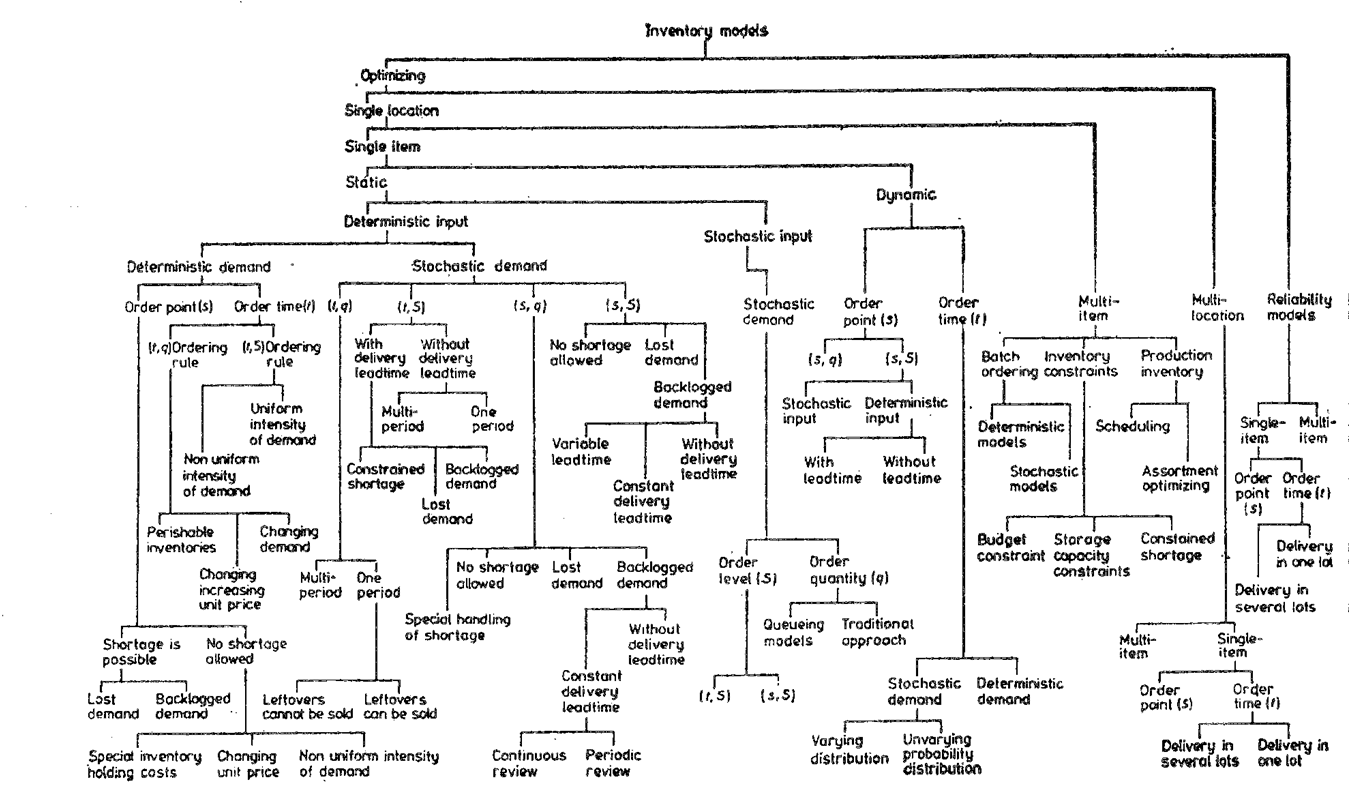
\includegraphics[width=\textwidth]{figures/chikan.png}
\caption{Decomposition of inventory models}
\label{fig:costs}
\end{figure}


\end{question}



\begin{question}
  Clearly, to make decisions it is important to have a good understanding
  of the relevant trade-offs. Interestingly, all these trade-offs can
  be reduced to three types of buffer. What buffers can that be?
  \begin{solution}
    Time, inventory, capacity, the three buffers. We urge you to read
    Section 6.2 and 6.3 of FP (edition 3) really critically. The ideas
    behind Figure 6.6 are very useful, and you can try to apply the
    underlying ideas to your case too when you have to make a choice
    for an inventory control policy, determine the policy parameter
    and do the sensitivity analysis.
  \end{solution}
\end{question}



\subsection{Modeling Examples}
\label{sec:examples}

We'll now use the check list we developed in one of the exercises
above to analyze a few simple inventory systems. We'll make a model
first, with symbols, because this helps in the communication about the
model and the documentation. Once we have a complete model we can
build it in excel and start simulating the system and evaluate
policies. Thus, the aim of the examples is to show you how to apply
the check lists to design and evaluate complete models. Note that
modeling is an art; as a consequence check lists can never be
complete, and there is also not one simple recipe to make a good
model. In that sense, the development of models is always somewhat
ad-hoc and unstructured, in fact, the development of the model helps
you to familiarize yourself with a situation you don't completely
understand. There is no way around except that you start modeling,
accept to make mistakes in the process, and test your assumptions and
modeling decision, improve your model after these test, and so on. The
proof of the pudding is in the eating\ldots and you don't know upfront
whether your model will be correct or not.

So we start with making a very simple model, a case description if you
will, and make it more complicated as we go along.  You are supposed
to follow the steps and implement them in excel, make graphs, compute
KPIs, and so on, to test your understanding of the approach to problem
solving we want you to learn.

\subsubsection{Systems with Backlog but without Inventory on hand}

\begin{question}
  Consider a production situation, a  machine for instance, that has a
  production capacity of  $c$ per day, e.g. $c=10$.  The daily demand,
  $d_i$ for day $i$, is always less then $c$. Is there a need for inventory?
  \begin{solution}
No, since $c\geq d_i$, the daily demand can be covered by production every day again.     
  \end{solution}
\end{question}

\begin{question}
  Let's assume that the machine can be switched on or off.  If on, it
  has capacity for $c$ jobs, if off it produces nothing.  Just to show
  the impact of the cost structure on the policy you would use to
  control the machine, suppose that the cost to operate the machine is
  $p$ per job, i.e., you only have to pay for the jobs you really
  processed. What what you do, that is, how would you control the
  machine?
  \begin{solution}
    Well, since it only costs money per job served, and we want to
    serve the jobs anyway, we can just switch on the machine whenever
    there is a job. In fact, we can leave it on always, for there is
    no penalty to have it switched on (or a reward for switching it
    off).
  \end{solution}
\end{question}

\begin{question}
  Henceforth we assume that it costs $p$ Euro per day, for instance
  $p=100$ euro, just to have the machine switched on, whether you use
  the capacity or not. What would you do now? When is such cost structure reasonable?
  \begin{solution}
    If $d_i=c$, i.e., the daily demand is always the same as the daily
    capacity, then there is not much you can do. However, if the
    demand is typically less than $c$, then it might be interesting to
    occasionally switch on the machine and let it produce all demand
    up to some time. That is, ensure that the machine capacity $c$ can
    be completely used when it is switched on. 

    If you have to hire or assign personel to operate the machine, you
    are typically confronted with a daily cost, whether the machine
    actually works or not.
  \end{solution}
\end{question}



\begin{question}
  Try to make a model for this case.  Use the check list to see what
  modeling choices you can (and have to) make.
  \begin{solution}
    Assume that customers are willing to wait for free.  Assume also
    that we want to serve all demand. (Note that this is a business
    decision. It might be profitable to reject some demand. ) Finally,
    assume that the demand process $\{d_i, i=1,2\ldots\}$ is given.

    You should realize at this point that capacity has a
    `lose-it-or-use-it' property. Unused capacity is lost, and any
    cost associated with that lost capacity is also lost.

    The best thing we can do then is to only switch on the machine
    when the total accumulated demand is larger than the capacity for
    a day.  Thus, if $d_1=2, d_2 = 5, d_3 = 4$, then take the capacity
    $c_1$ for day 1 equal to 0, and likewise for day 2. However,
    $c_3 =10$. 
  \end{solution}
\end{question}


\begin{question}
  Implement the model in excel, and compute the total cost for the
  following demand process: $d = 2, 5, 4, 5, 0, 2, 3, 8, 9, 1, 1, 3$.
\begin{solution}
  Take $c_i$ as the capacity of day $i$. In our case $c_i=c=10$ if
  production is on, and $c_i=0$ if production is off.  Realize that
  any unfilled demand is transferred to the next period. To keep track
  of total demand, let's call $B_i$ the total demand in the system
  waiting for the machine to make their item. Then, if the machine
  does not produce anything in day $i$, the unfulfilled demand at the
  end of day $i$ is $B_i=B_{i-1}+d_i$, i.e., we start day $i$ with
  unfulfilled demand $B_{i-1}$ and then the demand $d_i$ arrives on
  day $i$. On the other hand, if the machine does produce, the total
  unfulfilled demand is $B_i = B_{i-1}-10 + d_i$, since we produce
  10. Thus, in general,
  \begin{equation*}
    B_i = B_{i-1} + d_i - c_i.
  \end{equation*}


  Typically, the unfulfilled demand is called \emph{backlog}. The
  interpretation is really simple, it is exactly the same as the queue
  of customers waiting for capacity. If you would apply this reasoning
  to the number of customers in queue waiting in a supermarket for
  service you would obtain exactly the same result.  

Thus, once and for all, backlogged customers, or backorders, are precisely the same thing as a queue of jobs or customers waiting for capacity. 

Realize also that this equation can be implemented straightaway in
excel.

Finally, observe that in the above we assume that when the machine is
on at day $i$, the capacity $c_i \leq B_{i-1}+d_i$, because otherwise
the $B_i<0$, and it is impossible to have a negative number of
customers in queue/backlog.
\end{solution}
\end{question}


\begin{question}
  Now we have to make a subtle choice. It might not be possible to use
  the capacity on day $i$ to handle the demand $d_i$ that arrives on
  day $i$. Of course, it also might be possible. In general it depends
  on the actual characteristics of the system which of the two
  assumptions is the more appropriate.  How would you absorb these
  choices into your model?
  \begin{solution}
    Suppose that the demand that arrives at day $i$ can also be covered by the machine in day $i$. It that case we only need to require that 
    \begin{equation*}
    B_i = \max\{B_{i-1} + d_i - c_i, 0\}.
    \end{equation*}
    Like this we are sure that the number of jobs in backlog is not
    negative.  

Otherwise, if the demand on day $i$ has to wait at least until day $i+1$, then
    \begin{equation*}
    B_i = \max\{B_{i-1} - c_i, 0\} + d_i.
    \end{equation*}

    Fill in these formulas with a set of numbers for the demand and
    implement it in excel to see what happens.  Start doing all kinds
    of experiments. How sensitive is the result to changes in $c$, for
    instance? What is a good rule to switch on and off the machine?
  \end{solution}
\end{question}

 


\begin{question}
  Can you find a set of formulas by which we can track the behavior of the backlog? 
  \begin{solution}
    Lets say that $S_i$ is the amount of demand sold/covered on day $i$. Henceforth we also assume that the demand on day $i$ \emph{can} be processed on day $i$. In this case, the amount sold is 
    \begin{equation*}
      S_i = \min\{B_{i-1}+d_i, c_i\},
    \end{equation*}
    since we cannot produce/sell more than the demand in backlog and
    we can also not sell more than the capacity.  The backlog is therefore,
\begin{equation*}
  B_i = B_{i-1}+d_i - S_i.
\end{equation*}
  \end{solution}
\end{question}

\begin{question}
  Suppose that we would decide to switch on the machine independently
  of the amount of jobs. Can you find a formula, to be implemented in
  excel, to compute the amount of capacity lost?
  \begin{solution}
The unused capacity $U_i$ is then
\begin{equation*}
  U_i = c_i - S_i,
\end{equation*}
because $c_i$ is the capacity we have, and $S_i$ is the amount we
used.

It is very important to memorize this scheme. Hence, once again:
\begin{align*}
      S_i &= \min\{B_{i-1}+d_i, c_i\}, \\
  U_i &= c_i - S_i, \\
  B_i &= B_{i-1}+d_i - S_i.
\end{align*}
Note that this scheme is quite simple in the sense that we have to
consider taking a minimum only once. 

  \end{solution}
\end{question}



\begin{question}
  For the rest of the course we need some important notation. What is the meaning of $\sum_{i=1}^j x_i$, and why is $h \sum_{i=1}^j x_i = \sum_{i=1}^j (hx_i)?$
  \begin{solution}
    \begin{align*}
      \sum_{i=1}^3 x_i &= x_1 + x_2 + x_3 \\
      \sum_{i=1}^j x_i &= x_1 + x_2 + \cdots +x_j \\
     h \sum_{i=1}^j x_i &= h(x_1 + x_2 + \cdots +x_j) = hx_1 + \cdots+hx_j = \sum_{i=1}^j h x_i.
    \end{align*}
  \end{solution}
\end{question}

\begin{question}
  Realize that in the previous problem we tacitly assumed that there
  is no cost associated with waiting.  In this case, we of course only
  switch on the machine when there is sufficient demand in
  backlog. But what would you do if there is a cost of waiting, for
  instance, if it costs $b$ per day to keep one unit of demand
  waiting. Then it might not be so efficient, in terms of costs, to
  only switch on the machine when the demand is sufficiently high to
  prevent lost capacity. Can you find an expression for the cost of
  keeping demand waiting and switching on the machine?
  \begin{solution}
    In excel we can build something really useful, the indicator
    function. It is 1 if $c_i>0$ and $0$ when $c_i=0$. Mathematically
    we write it like $1\{c_i>0\}$.  

    With this it is easy to compute the total cost up to some day
    $j$. On day $i$ we pay $b B_i$ if there are $B_j$ units of demand
    in backlog, and we pay $p 1\{c_i>0\}$ for the production. Thus,  the total cost up to time $j$ must be 
    \begin{equation*}
      b\sum_{i=1}^j B_j + p \sum_{i=1}^j 1\{c_i > 0\}.
    \end{equation*}

  \end{solution}
\end{question}

\begin{question}
  Assume next that we get a profit $r$ per unit demand sold/produced, then
formulate the reward structure.
  \begin{solution}
    The profit function up to time $j$ is
    \begin{equation*}
     r \sum_{i=1}^j S_j - b \sum_{i=1}^j B_j - p \sum_{i=1}^j 1\{c_i>0\}, 
    \end{equation*}
    i.e., the sum of the total profit minus the cost of backlog minus
    the cost of switching on the machine (recall $c_i = 0$ is the
    machine is off and $c_i = 10$ if on.).

  \end{solution}
\end{question}

\begin{question}
  It might be that the business context requires that the amount of
  backlogged demand should not exceed some critical level $a$ say too
  often. Can you find an expression to estimate how often such an
  event occurs with excel for a given set of demands?
  \begin{solution}
    When $B_i>a$ we are `in trouble. Thus, to count how often this happen, we can compute
    \begin{equation*}
      \sum_{i=1}^j 1 \{B_i > a\}.
    \end{equation*}
  \end{solution}
\end{question}

\begin{question}
  Observe that in the previous exercise we only counted the number of
  periods in which the backlogged demand exceeded some level $a$. It
  might also be of interested to compute the total amount of
excess  backlogged demand. What can be an appropriate formula for this? 
\begin{solution}
    When $B_i>a$, the amount in excess is $B_i$. Thus, 
    \begin{equation*}
      \sum_{i=1}^j B_i 1 \{B_i > a\},
    \end{equation*}
  is the amount we want to compute. 
\end{solution}
\end{question}

\begin{question}
  What is the total amount of demand backlogged? 
  \begin{solution}
    In the previous expression set $a=0$. 
  \end{solution}
\end{question}

\begin{question}
  If you like, you can try to formulate an optimization problem for
  the problem on how much to produce. .
  \begin{solution}

    TBD = to be done = unfinished. You can always skip exercises that
    are marked as TBD.

The decision variables are whether we switch on the machine at the days, i.e., $c_1, c_2, \ldots, c_j$. 

The constraints are:

\begin{align*}
c_i &\in \{0, 10\}, \\
      S_i &= \min\{B_{i-1}+d_i, c_i\}, \\
  B_i &= B_{i-1}+d_i - S_i.
\end{align*}

In Section 16.2 of Factory Physics it is shown how to optimize this
problem in excel for \emph{given} demand, i.e., if we know the
demands.  If we don't know the demands, then things become quite a bit
different.

  \end{solution}
\end{question}



\subsection{Systems with Inventories}
\label{sec:inventories}

\begin{question}
  In the previous problem we tacitly assumed that customers are
  prepared to wait.  What if this is not the case, i.e., you serve
  them right away, or they leave. Suppose we don't want demand to
  leave. What can you do about this?
  \begin{solution}
    We assumed that demand arriving on a day cannot be covered/served
    on that same day. If we don't have inventories, all demand will be
    lost. Thus, the only way out seems to be to start keeping real
    inventories. (Realize that up to now we only considered backlogged
    demand, which is, in a sense, negative inventory.) 
  \end{solution}
\end{question}

\begin{question}
  So, let us assume for the remainder that it is possible to invest in
  inventory. How much inventory do we need? Assume that the production
  of the machine can be used to satisfy the demand for that day. 
  \begin{solution}
    If we don't want to lose any demand, and if demand is capped by
    some number, e.g.  $\bar d$ is such that $d_i \leq \bar d$ for all
    $i$, then we are always safe by keeping $\bar d$ items on hand,
    i.e., $\bar d-c$ on shelf at the start of the day
  \end{solution}
\end{question}

\begin{question}
  Write $I_i$ for the inventory at the end of day $i$.  
% We now need to
%   make an assumption about how $\bar d$ compares to the maximal
%   machine capacity $c$. 
  Let us also we assume that $\bar d \leq c$ (that is, the machine can
  always produce more than the maximal demand).  Use this to come up
  with a rule to decide when to switch on the machine.
  \begin{solution}
    We need at the start of the day an inventory of $\bar d$ to cover
    the demand. Realize that the inventory at the start of the day is
    the same as the inventory at the end of the previous
    day. Therefore, for day $i$ we want that $I_{i-1} = \bar d$. If,
    however, $I_{i-1}<\bar d$, we need to produce. But now recall that
    what we produce on a day cannot be used to serve the demand for
    that day.  Thus, we need to prevent that $I_{i-1}<\bar d$, because
    if that happens, we might be one day too late.

    Realize that also that, by assumption, the machine has sufficient
    capacity to cover the maximal demand of one day. Thus, we are safe
    if we produce whenever $I_{i-1} <2 \bar d$, and we don't have to
    be concerned with loss.  

All in all, 
    \begin{align*}
      c_i &= c1\{I_{i-1}< 2\bar d\}, \\
      I_i &= I_{i-1} -d_i + c_i. 
    \end{align*}
  \end{solution}
\end{question}

\begin{question}
  Try to make a cost model. Assume that we charge for inventory at the
  end of the day.  There is a cost $h$ to have one item on hand at the
  end of the day.
  \begin{solution}
    The cost of inventory is $\sum_{i=1}^j h I_{i}$ and the cost of
    production has been given before: $p\sum_{i=1}^j 1\{c_i>0\}$.

    Observer there is no backlog, and also no lost demand. Hence,
    these terms do not add to the cost.
  \end{solution}
\end{question}

\begin{question}
  If, however, $c< \bar d$, the situation changes quite
  dramatically. Suddenly, to prevent loss we need more than $\bar d$
  of inventory at the start of the day, because if the inventory
  becomes below $\bar d$, we might not be able to replenish it
  sufficiently for the next day. What would you do?
  \begin{solution}
    First of all, we observe that it is impossible to prevent lost
    sales under all circumstances if demand is stochastic. It can
    happen that we have 10 days in row, say, that the maximal demand
    arrives. We need already quite a bit of inventory to cope with
    this. In general, in case demand is stochastic, any amount of
    demand can arrive, so that we cannot protect ourselves always
    against loss. 

    Thus, we need \emph{safety stock} to compensate for the fact that
    our production cannot cope with the maximal daily demand.

    We also need to assume that the capacity of the machine is higher
    than the average demand, for otherwise we will have quite a bit of
    loss. 

    Tuning the safety stock to minimize cost is an issue we'll address
    next. 


  \end{solution}
\end{question}

\begin{question}
  What would happen if there is a number of periods between the moment
  the items are produced and that the items become available for
  sale.  How would you organize your production plan, i.e., the periods in which to to decice to switch on the machine? 
  \begin{solution}
    TBD.
  \end{solution}
\end{question}

\begin{question}
  Can you relate the production of the machine to a situation in which
  inventory is replenished by a supplier?
  \begin{solution}
    The production amount $c$ is equivalent to a constraint on the
    amount that can be ordered from a supplier. The time between
    deciding to produce and the moment an item is available for
    customers is equivalent to a lead-time between ordering a
    replenishment order and receiving the replenishment.
  \end{solution}
\end{question}

\subsection{Systems with loss}
\label{sec:real-that-prev}

\begin{question}
  Lets step back a bit\ldots In fact, we do not need to keep at least
  $\bar d$ items of on hand inventory. What if we would carry less
  inventory, and accept a bit of loss?  After all, the cost may
  decrease if we allow for this situation. Can you make a model for
  this situation, that is, a model that can cope with loss?
  \begin{solution}
    This is an interesting situation. First assume there is no
    loss. Then the total amount we produce is the same as the total
    demand. The production cost, i.e., cost to switch on the machine
    is relatively simple. It is just the total demand divided by the
    daily production capacity $c$ and then times the production cost
    $p$ per day, in other words, the total cost of production is
    $p\sum_{i=1}^j d_i/c$.

    If there is loss, however, we need to produce less (because some
    demand is lost) and we also can keep lower inventories. Thus,
    accepting a bit of loss may be interesting as we get cost
    reductions in two aspects: less production and lower inventories.

    A simple policy is to switch on production when the inventory
    $I_{i-1}\leq r$ for some (base-stock) level $r$. 

Observe also that our sales $S_i$ in day $i$ may need not be equal to the demand $d_i$,  as we cannot sell more than what we have on stock. Thus,
    \begin{align*}
      c_i &= c 1\{I_{i-1} \leq r\}, \\
      S_i &= \min\{d_i, I_{i-1}\}, \\
      L_i &= d_i - S_i, \\
      I_i &= I_{i-1} -S_i + c_i, 
    \end{align*}
    where $L_i$ is the lost demand. Note that as $S_i \leq d_i$,
    $L_i \geq 0$ (i.e., we don't run into the trouble of negative lost
    demand).
  \end{solution}
\end{question}

\begin{question}
  What would be the cost of this situation, assuming that it costs $k$
  per unit of demand lost? 
\begin{solution}
  \begin{equation*}
    \sum_{i=1}^j \left(h I_{i} + k L_i + p1\{c_i>0\}\right).
  \end{equation*}
\end{solution}
\end{question}

\begin{question}
  How would you use the results of the previous two exercises to tackle the case in which the machine capacity is less than $\bar d$?
  \begin{solution}
    As a matter of fact, we don't have to change anything. We can use
    the results right away. Observe that the control parameter is $r$,
    i.e., the re-order level. By trying different choices for $r$ we
    can compute/simulate the inventory level, loss and so on, and the
    total cost. The best $r$ minimizes this cost.

    Realize that, formaly, it is not necessary that $c$ is larger than
    the mean demand. If it is less, simply more loss will occur.
  \end{solution}
\end{question}


\begin{question}
  Use the numbers $\{L_i\}$ and $\{S_i\}$ to estimate the fill rate,
  the loss rate, and the service cycle level.
\begin{solution}
The total demand is
\begin{equation*}
 \sum_{i=1}^j d_i, 
\end{equation*}
and the total amount of demand served/sold is 
\begin{equation*}
 \sum_{i=1}^j S_i.
\end{equation*}
Hence, the fill rate is given by
\begin{equation*}
  \frac{\sum_{i=1}^j S_i}{\sum_{i=1}^j d_i}.
\end{equation*}
The service cycle level is the fraction of periods in which loss did not occur:
\begin{equation*}
  \frac 1 j \sum_{i=1}^j 1\{L_i=0\}, 
\end{equation*}
i.e., the average number of days in which the system did not run out of stock.

Note that these two KPI's are not the same. 
\end{solution}
\end{question}

\begin{question}
  Is the service cycle level a good measure for the  amount of loss?
  \begin{solution}
    No, not really. It might be that a small shortage occurs nearly
    every period. Then the fraction of periods without loss, i.e., the
    cycle service level, is very low. However, since only a small
    portion of the demand is lost, the fill rate may be pretty high. 

    So, why then use the service cycle level, and why not always use
    fill rate? (Realize that fill rate does relate to money, but
    service cycle level doesn't.) Well, the answer is easy. People,
    managers in particular, tend to understand cycle service level
    better, and cycle service level is easy to compute. The fill rate
    is just a bit more complicated. 
  \end{solution}
\end{question}

\begin{question}
  How long does demand spend in backlog on average?
  \begin{solution}
    We can use Little's law to get an approximate value for this, but
    it takes some time to see how to do it. So, let's review Little's
    law. Consider some input-output system---it doesn't quite matter
    what system, as long any item/job/customer that enter the system
    eventually departs from the system.  Let jobs arrive at rate $r_a$
    per unit time. The average time a job spends in the system is $W$
    and the (time) average number of jobs in the system is $L$. Then
    the law states that $L = r_a W$.  Thus, the average time jobs
    spend in the system is $W = L/r_a$.

    First consider the entire system. The rate at which jobs enter must be roughly 
    \begin{equation*}
      r_a = \frac 1 j \sum_{i=1}^j d_i,
    \end{equation*}
    i.e., the average demand rate. The time-average of the amount of
    demand in backlog is roughly
    \begin{equation*}
    \bar B \approx \frac 1 j \sum_{i=1}^j B_i.
    \end{equation*}
    Hence, the average time demand spend in backlog must be
    $W =  \bar B /r_a$.

    Now notice that this is the average waiting time averaged over
    \texttt{all} demand, thus, also the demand that actualy does not
    have to wait. This number is therefore only partially interesting:
    it doesn't tell how long, on average, a backlogged customer has to
    wait. (Only when a customer has to wait, s/he is interested in how
    long the waiting will take. Customers that don't have to wait, are
    not interested in `knowing how long they have to wait'.) Thus, we
    need to repair for this. But how? 

    Well, we can again use Little's law, but now apply it to the
    `system' that is entered only by the backlogged customers.  So,
    how much demand enters this system?  A first guess is all the demand that leaves backlog behind:
    \begin{equation*}
      \sum_{i=1}^j d_i 1\{B_i > 0\}.
    \end{equation*} 
 

    Is this correct? What if $d_i=7$, $B_{i-1}=8$ and $c_i= 10$. Then
    $B_{i} = 8+7-10 = 5$. Thus, assuming FIFO service of backlogged
    demand, of the 7 demands entering, only 5 will be backlogged, the
    rest, i.e., 2, will be served on day $i$ itself. That means that
    $d_i 1\{B_i>0\}$ must overcount the amount of demand that is
    backlogged. Another example might help to get the right number. If
    $B_{i-1}=10$, the $B_i=7$, hence all demand on day $i$ is
    backlogged. But if $B_{i-1}=2$, then $B_i = 0$ and no demand is
    backlogged. Thus, only if $B_i\geq d_i$ all demand is backlogged,
    otherwise $B_i$ is backlogged, in other words, 
    \begin{equation*}
      d_{i,b} = \min\{d_i, B_i\}
    \end{equation*}
    gets backlogged. The rate of  backlogged demand is then
    \begin{equation*}
      r_{a,b} =
      frac 1 n \sum_{i=1}^j d_{i,b} = frac 1 n \sum_{i=1}^j \min\{d_i, B_i\}.
    \end{equation*}
    With this we see that the average time backlogged demand stays in
    backlog must be
    \begin{equation*}
      W_b  = \frac{\bar B}{r_{a,b}}. 
    \end{equation*}

    Note that $r_{a,b} < r_a$, hence $W_b > W$, as it should.

    It would be interesting to check the above with simulation, and
    see whether any mistakes remain. 

    Note also that we take the average over some $j$ periods. This is
    of course not the same as the real long-run average (i.e., the
    average taken over an infinite amount of time). As Little's law is
    only valid asymptotically (taking an infinite amount of time), the
    above relations can only be approximately correct.
    
  \end{solution}
\end{question}

\subsection{Systems with full backlogging}
\label{sec:systems-with-backlog}

\begin{question}
  Assume that, in case of demand cannot be covered by on-hand
  inventory, (i.e., the stock is empty), it is backlogged. Make a
  model of the behavior of the system and a cost function.
  \begin{solution}
    First of all, observe that we can absorb on-hand inventory and
    backlog into one concept. We write $I_i$ for the on-hand inventory
    at the end of the day if the on-hand inventory is positive and we
    set $I_i=-B_i$ if there is backlog. Thus, when $I_i$ is negative,
    it means that $I_i$ demand is in backlog.  Observe that, as a
    consequence, it cannot happen that there is demand in backlog but
    there is also positive on-hand inventory at the same time.

    We can numerous assumptions on how to model this situation. None
    is particularly right or wrong, it simply depends on the specifics
    of the situation we need to model. Assume for instance that we
    switch on the machine when the inventory is below or at some level
    $r$. The inventory level must go down with the demand and up with
    the amount produced:
    \begin{align*}
      I_i &= I_{i-1}-d_i + c_i \\
c_i &= c 1\{I_{i-1} \leq r\}.
    \end{align*}

    For the revenues we can also make at least two choices: do we get
    the money when the customer decides to `enter the system',
    irrespective of being backlogged, or do we get the money when we
    actually satisfy the demand. Here we model the latter situation.
    If $I_i\geq 0$, we know that we have met all demand for that
    day. Thus, in this case, the sales for day $i$ must be
    $S_i = d_i+B_{i-1}$, that is, the demand for day $i$ plus all
    backlogged demand $B_{i-1}$, if any. If, however, $I_i <0$, then
    we cannot have met $d_i$ entirely. Since we produced $c_i$ on that
    day, $S_i = c_i$, i.e, we must have sold $S_i$. 

    Note that we assume in the above that any items produced in excess
    of $r$ is kept in inventory. If this is cannot be the case (due to
    space restrictions for instance), the above recursions need to be
    changed.

    We leave it to you to consider other interesting cases and adapt
    the above models to your settings.

  \end{solution}
\end{question}


\begin{question}
  We have not yet discussed models with positive lead times. 
  \begin{solution}
    TBD.
  \end{solution}
\end{question}


%%% Local Variables:
%%% mode: latex
%%% TeX-master: "notes_all"
%%% End:


\section{Demand Characterization}
\label{sec:character}
%\textit{Recommended reading:} FP Section 13.3. FP describes various methods and concepts related to demand forecasts, e.g. regression, moving-averages, exponential smoothing, trends and seasonal patterns, measures of forecast accuracy. We expect you to be familiar with these basic methods. 

Any successful inventory management practice starts with projecting the demand that will realize in the future. This section is devoted to understanding demand processes and forecasting future demands. 

\subsection{The Role of Demand Forecasts}

\begin{question}
Why do we need to forecast demands?

\end{question}

  \begin{solution}
    We often need to replenish inventories ahead of demand, i.e. before observing the demand. As such, projection of future demands, or in other words, forecasting, is the foundation upon which replenishment plans are made. 
    
    Of course, in some cases, you might have the complete demand information before it is realized. For instance, your customers may let you know in advance, say a week before, they actually demand an item. In such cases, you can safely assume that you know the demand over the next week with certainty. Thus there will be no need for forecasting -- at least not for the upcoming week. 
  \end{solution}

\begin{question}
Why inventories are replenished ahead of demand?
\end{question}

  \begin{solution}
    There is a variety of reasons. For instance, often there is an order lead time, i.e. the lag between the time that an order is placed and the time inventory is actually replenished. Another reason is that it could be preferable to place larger orders due to economies of scale, e.g. quantity discounts or fixed ordering costs. 
    
	Let us consider an inventory system where replenishments are done on a daily basis. That is, you place an order at the end of every day, and receive it the next day in the morning. It appears that there is no lead time here. But anyway you are exposed to demand uncertainty over the day. That is, you must have enough in the morning to cover the demand over the day -- which has not yet been realized. 
  \end{solution}


\begin{question}
What should we expect from demand forecasts?

\end{question}

  \begin{solution}
	For most products, demand is inherently uncertain. As such, exact demand values cannot be forecasted. The aim of forecasting therefore is to capture the structural properties of demand, such as its average, rather than the demand itself.  
	

  \end{solution}

\begin{question}
Which factors come into play in forecasting, i.e. what is the input?

\end{question}

  \begin{solution}
    The input of forecasting is comprised of all type of information regarding historical demand as well as the future demand. These involve, among others, objective factors such as past demand data, trend and seasonality, prices, promotions, dependencies among different products, as well as subjective factors such as sales force surveys and expert opinions.     
  \end{solution}


\begin{question}
What is the output of a forecast?

\end{question}

  \begin{solution}
    The output of a forecast is a set of data points for future demands as well as a measure that explains to which extent actual demands will deviate from their forecasts.
  \end{solution}


\begin{question}
How forecasts are used inventory management?

\end{question}

  \begin{solution}
	Inventory management is done through inventory control policies. The output of forecasts are used in designing inventory control policies and determining the parameters of these policies.
  \end{solution}


\begin{question}
How much effort should be put into forecasting?

\end{question}

  \begin{solution}

	Because obtaining a highly accurate forecast is costly and time consuming, one should consider the trade off between its benefits and costs. The benefit of a forecast lies in how sensitive inventory costs are to forecast accuracy. 
	
	In inventory systems with a large number of SKU's it is simply not possible to put a lot of effort into forecasting. But for very expensive items which are sold rather infrequently (say a diamond ring or an aircraft spare part) the value of having a better forecast can be very high. This is mainly due to the cost of the mismatch between supply and demand, i.e. stock-out costs as well as holding costs are very high. 
	
	As a rule of thumb, one should avoid overly naive forecasting approaches as well as excessively complicated ones. 
  \end{solution}


\begin{question}
Consider the EOQ problem (for the sake of simplicity neglect the unit production cost). Now assume that the demand $D$ that is used in computing the order quantity is off by a factor of $\Delta$. That is, actual demand happens to be $D(1+\Delta)$ rather than $D$. 
\begin{enumerate}
\item Derive an expression to illustrate the cost of using the wrong demand value as compared to the optimal cost. 
\item Plot the cost error for $-0.5\leq \Delta\leq 0.5$ and solution on the extent of the cost error.
\item Comment on the implications of this thought experiment with respect to the importance of forecast accuracy.
\end{enumerate}
\end{question}

  \begin{solution}
\begin{enumerate}
\item Because the order quantity is set assuming that demand is $D$, it will be $Q=\sqrt{2AD/h}$. If one were to know the real demand $D(1+\Delta)$, then the optimal order quantity would be $Q^*=\sqrt{2AD(1+\Delta)/h}$. 

Observe that $Q=Q^*\sqrt{1+\Delta}$. That is, if demand is off by 20\%, then the order quantity will be off by only 9.5\%.

When actual demand is $D(1+\Delta)$, the costs of using order quantities $Q^*$ and $Q^*\sqrt{1+\Delta}$ will be 
\begin{align*}
C^* = AD\frac{1+\Delta}{Q^*}+ h\frac{Q^*}{2} \quad \text{ and } \quad C = AD\frac{1+\Delta}{Q^*}\frac{1}{\sqrt{1+\Delta}}+h\frac{Q^*}{2}\sqrt{1+\Delta}
\end{align*}
respectively. Because, $Q^*$ is the optimal order quantity when demand is $D(1+\Delta)$, we have $C^*/2=AD(1+\Delta)/Q^*=hQ^*/2$. Thus, 
\begin{align*}
C & = C^*\frac{1}{2}\left(\frac{1}{\sqrt{1+\Delta}}+\sqrt{1+\Delta}\right)
\end{align*}
\item See Figure~\ref{fig:costerror}. We observe that if demand is underestimated by 50\%, the cost error is 6\%; and if it is overestimated by 50\%, the cost error is 2\%. The cost penalty does not look that serious on the overall.

\begin{figure}
\centering
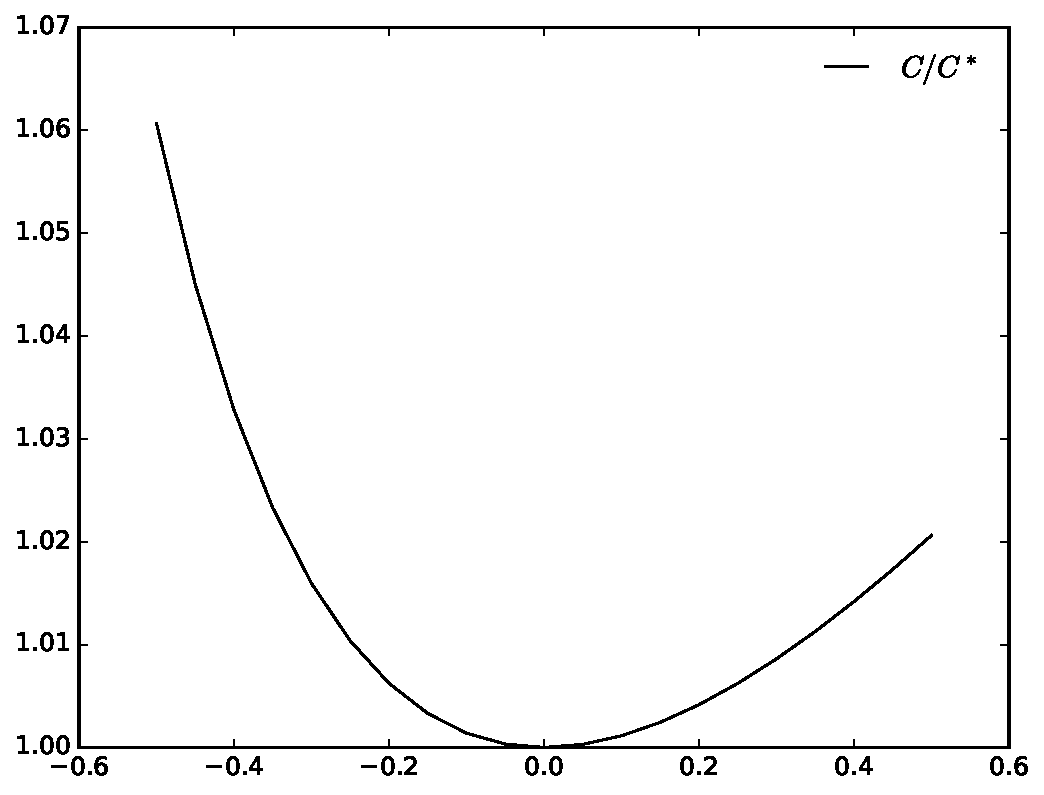
\includegraphics[width=.5\linewidth]{figures/Figure_1.pdf}
\caption{Cost error}
\label{fig:costerror}
\end{figure}

\item The EOQ cost is rather insensitive to the demand for which the order quantity is based upon. As such, a highly accurate forecast, although preferable, is not necessary. 
\end{enumerate}
    
  \end{solution}


\begin{question}
Discuss which underlying assumptions of the EOQ model makes it insensitive to the demand uncertainty. 
\end{question}

  \begin{solution}
  The EOQ model assumes that all demand can be served in time. That is because the inventory will be replenished instantaneously whenever the inventory level drops down to zero. In that sense, not using the optimal order quantity effect the trade-off between the ordering and holding costs, but not the service quality. Often in stochastic inventory control systems there is a cost associated with providing a certain quality of service. This is not reflected on the EOQ model.
  \end{solution}

\subsection{Forecasting Methods}

\begin{question}
What type of methods are used in forecasting?
\end{question}

  \begin{solution}
    There are two types of forecasting methods: qualitative and quantitative methods. The former use subjective inputs such as expert opinions. These are more apt for long-term forecasts where past data are not sufficient to predict the future, e.g. where technological breakthroughs may play a significant role. The latter use objective inputs such as past data. These are more suitable for short-term forecasts where numerical measures of the past observations can explain the future with a sufficient degree of accuracy. 
   \end{solution}
   
\begin{question}
What type of forecasting methods are used in inventory management?

\end{question}

  \begin{solution}
	In most practical cases, the number of SKU's is too large to implement SKU-specific forecasting methods. As such, often automatized forecasting procedures that work solely with past quantitative data are employed for demand forecasting in inventory management. There are two types of quantitative forecasting models: causal models and time-series models.

   \end{solution}
   
\begin{question}
How do causal forecasting models work?

\end{question}

  \begin{solution}
    Causal models assume that demand is a function of some other parameters (e.g. price, market size, time, and weather). Here are some examples. The demand for diapers this year is a function of last years birth rates. The demand for FC Groningen jerseys is a function of the team and individual player performances. 

Once all the factors that explain demand are identified, one can easily predict demand given the values of these parameters. 

Let $X_1,X_2,\ldots,X_m$ be the values of the parameters explaining the demand. Then, assuming that each parameter effects the demand linearly and independently, the forecast would be 
\begin{equation*}
Y = b_0 + b_1 X_1 + \ldots + b_m X_m
\end{equation*}
where $b_0,b_1,\ldots,b_m$ are the constants defining the demand function. 

Here, the challenge is to find a function (i.e. the parameters values $b_0,b_1,\ldots,b_m$) that best forecasts the demand. This is often done by using past data via regression analysis -- a highly accessible tool as it is available in almost all spreadsheet programs. 

An important drawback of using a causal model is that the values of those parameters explaining demand should be readily available. Otherwise, one needs to to forecast them before forecasting demand. For instance, if the weather is a factor effecting the demand, then one needs the forecast the weather before forecasting the demand.    

  \end{solution}


\begin{question}
How do time-series forecasting models work?

\end{question}

  \begin{solution}
Time-series models assume that past demand data are almost sufficient to forecast future demands. As such, all causal factors are neglected with the rationale that such factors tend not to change in the short-term. 

If time is treated as a discrete entity (i.e. days, weeks, or months), then, assuming that period $t$ is the actual period, a time-series model takes all past demand observations $A(1),A(2),\ldots,A(t)$ and generates forecasts $f(t+1),f(t+2)\ldots$ for future demands. 

As compared to causal models, time-series models are more commonly used in inventory management because they are very simple, do not require much data, and (often) reliable. Also, they are easy to use and integrated in many spreadsheet applications.
  \end{solution}


\begin{question}
How exactly do time-series models forecast demand by solely using past demand data?

\end{question}

  \begin{solution}
There are two approaches towards time-series forecasting: moving-averages and exponential smoothing. The main idea behind both approaches is to put emphasis on the recent demand data when making a forecast, based on the belief that recent data better explains actual demand.

\textit{Moving-Averages:} 
Here, one simply averages recent demand data to forecast demand. Let us define 'recent' as the last $m$ periods. Then, the moving average approach forecasts the next periods demand as follows:
\begin{align*}
F(t) & = \frac{\sum_{i=t-m+1}^t A(i)}{m} \\
f(t+\tau) & = F(t) \quad \tau = 1,2,\ldots
\end{align*}
As can be observed, we first compute the term $F(t)$. This is often referred to as the demand 'level'. Then we use the demand level to forecast demands in future periods. Notice that our forecasts for all upcoming periods $f(t+1),f(t+2),\ldots$ are the same and they are all equal to the level $F(t)$. 

\textit{Exponential Smoothing:} 
Here, all past observations are used (rather than only the recent ones) while placing gradually decreasing weights on observations further into the past. Let us assume that that the weight put on the most recent observation is $\alpha$ ($0<\alpha\leq 1$). Then, the exponential smoothing approach forecasts future demands as follows:
\begin{align*}
F(t) & = (1-\alpha)^0 \alpha A(t) + (1-\alpha)^1 \alpha A(t-1) + (1-\alpha)^2 \alpha A(t-2) + \ldots \\
& = \alpha A(t) + (1-\alpha) F(t-1) \\
f(t+\tau) & = F(t) \quad \tau = 1,2,\ldots
\end{align*}
Observe that the demand level in period $t$ is simply a linear combination of the actual demand $A(t)$ and the demand level $F(t-1)$ in the previous period. 


Both moving-average and exponential smoothing models are easy to implement in a spreadsheet. We suggest you to implement and play around with those models by using the examples from FP.
  \end{solution}


\begin{question}
What is the importance of the parameters used in time-series forecasting models?

\end{question}

  \begin{solution}
It is important to see that parameter $m$ of the moving average approach and parameter $\alpha$ of the exponential smoothing approach both stand for the same purpose: to define how responsive the forecast is to recent changes in the demand. For instance, a sudden change in the demand pattern will have a more significant impact in a moving average forecast if $m$ is smaller, and in an exponential smoothing forecast if $\alpha$ is larger. Here, the main concern is to identify whether such changes are random fluctuations or actual changes in the demand pattern. 
    
      \end{solution}


\begin{question}
How the smoothing parameter is chosen in exponential smoothing models?

\end{question}

  \begin{solution}
	It depends on the KPI's that are deemed to be important for the case on hand. A classical approach is to set smoothing parameters to minimize forecast errors. That is, the error that would have been observed so far if a particular smoothing parameter were used. 	We will elaborate on this more later on. This approach, however, focuses solely on the demand. However, one can also choose a smoothing parameter that optimizes the performance of the inventory policy that is planned to be used. This would lead to an integrated forecasting and inventory control framework.
	
  \end{solution}

\subsection{Trends and Seasonality}

\begin{question}
The standard time-series forecasting models provide the same forecast for all periods in the future. Does it make any sense? 
\end{question}

  \begin{solution}
    It depends. So far, we have not considered any reason that may lead to a persistent demand behavior over time. Therefore, it is logical that our forecasts for future demands are all equal to the current demand level $F(t)$ and do not involve any fluctuations over time.     
      \end{solution}


\begin{question}
What factors may lead to a persistent demand behavior over time?

\end{question}

  \begin{solution}
    There are virtually unlimited number of factors. But the most common ones are trends and seasonal variations. Here, trends refer to movements in demand in one direction (i.e. increasing or decreasing over time) and seasonal variations are movements in demand periodic to a calendar (e.g. peaks or bottoms on weekends, during summer time, or at Christmas).
    
    Besides these common factors, we know that all products have a life cycle. We observe low demands when a product is first introduced to the market. The demand increase as the product penetrate the market and level off once the product is mature. Towards the end of the product life cycle, demands decrease and the product die out eventually. 
      \end{solution}


\begin{question}
Is it possible to account for trends and seasonal variations in time-series forecasting models?
\end{question}
   
  \begin{solution}
   Yes. The effects of such factors can be regarded as demand components. Then the value of each of these components can be forecasted, and the demand itself can be forecasted by using these forecasts. 
     \end{solution}
     
\begin{question}
How do we capture trends in time-series forecasting models?
\end{question}

  \begin{solution}   
   Here, we illustrate how this can be done with an exponential smoothing model. Yet the presented ideas can easily be extended to any other model. 
 
   Let us consider a demand with linear trend (demand moves by a constant every period). Here, we should keep track of the demand level $F(t)$ as well as the trend $T(t)$ time by exponential smoothing. We use smoothing constants $\alpha$ and $\beta$ for demand level and trend, respectively. Then, we can revise the exponential smoothing model as follows:
\begin{align*}
F(t) & = \alpha A(t) + (1-\alpha) [F(t-1)+T(t-1)] \\
T(t) & = \beta [F(t)-F(t-1)] + (1-\beta) T(t-1) \\
f(t+\tau) & = F(t) + \tau T(t) \quad \tau = 1,2,\ldots
\end{align*}
Here, the level is once again a linear combination of the actual demand and its forecast made in the previous period. The trend, on the other hand, is a linear combination of the actual change in the level and the trend in the previous period. The forecast of $\tau$ periods ahead is then the sum of the current level plus $\tau$ times the trend. 

The same reasoning explained here can be applied to trends that are not linear. To practice, you can try and extend this model to capture another case where demand is moving by a percentage rather than a constant in each period, e.g. every period it increases by 5\%. 

  \end{solution}
  
\begin{question}
How do we capture seasonal variations in combination with trends in time-series forecasting models?

\end{question}

  \begin{solution}   
   Here, we illustrate how this can be done with an exponential smoothing model. Yet the presented ideas can easily be extended to any other model. 
 
Let us consider a demand with a linear trend and a multiplicative seasonal factor (demand moves by a factor in each period in the season), and assume that there are $N$ seasons. Here, we should keep track of not only the demand level $F(t)$ and trend $T(t)$, but also the seasonality multiplier $c(t)$, all by means of exponential smoothing. We use smoothing constants $\alpha$, $\beta$, and $\gamma$ for demand level, trend, and seasonality multiplier, respectively. In this case, the exponential smoothing model can be revised as follows:
\begin{align*}
F(t) & = \alpha  \frac{A(t)}{c(t-N)}+ (1-\alpha) [F(t-1) + T(t-1)] \\
T(t) & = \beta [F(t)-F(t-1)] + (1-\beta) T(t-1) \\
c(t) & = \gamma \frac{A(t)}{F(t)} + (1-\gamma) c(t-N) \\
f(t+\tau) & = [F(t) + \tau T(t)] c(t+\tau-N) \quad \tau = 1,2,\ldots
\end{align*}
The novelty here is to strip the seasonality factor from the demand. This is done by dividing actual demand by the seasonality factor (from the last period that belongs to the same season), and using the resulting seasonality-free demand in computing the level. Apart from this, the computation of the level and the trend remains intact. The seasonality factor is a linear combination of the ratio of actual demand to demand level -- which reflects the actual seasonality factor and the factor that was computed for the same season last time. Then, the forecast of $\tau$ periods ahead is the sum of the current level plus $\tau$ times the trend, all scaled by the seasonality factor from the last period that belongs to the same season with the forecast period. 

The model mentioned above is often referred to as the Winter's model. Its main assumption with respect to seasonality is that the seasonality factor moves the demand by a percentage. To practice, you can try and adapt this model to capture another case where demand is moving by a constant rather than a percentage in each season, e.g. it is 100 units more on Saturdays. 

  \end{solution}
  
  
\subsection{Intermittent Demand}

\begin{question}
It is often the case for some products (for instance spare parts) that for long intervals of time there is no demand. Then, for instance, if we use a moving-average model we can end up with a forecast of zero. Does it make any sense to use standard time-series forecasting techniques for such products?
\end{question}

  \begin{solution}
  If demand data has a significant number of periods with zero demand, then the demand for the underlying product is said to be 'intermittent'. 
  
  One can make use of standard time-series forecasting techniques for such products. However, to that end, 'time' needs to be treated differently. The main idea here is to forecast the non-zero demand size and the inter-arrival time between successive non-zero demand periods separately, both using, for instance, exponential smoothing. The forecasts of these two should be updated only after demand occurrences (rather than each period). 
  
  Let us consider an intermittent demand. We index arrivals over time by $n$, and denote the size and the inter-arrival time of the $n$th arrival by $Z(n)$ and $P(n)$, respectively. We should keep track of the level of the demand size $F_Z(n)$ and the level of the inter-arrival time $F_P(n)$. We use the respective smoothing constants $\alpha_Z$ and $\alpha_P$ for the level of demand size and inter-arrival time. Then, we can construct an exponential smoothing model as follows:
\begin{align*}
F_Z(n) & = \alpha_Z Z(n) + (1-\alpha_Z) F_Z(n-1) \\
F_P(n) & = \alpha_P P(n) + (1-\alpha_P) F_P(n-1) \\
f(n+\tau) & = F_Z(n)/F_P(n) \quad \tau = 1,2,\ldots
\end{align*}   
   Here, assuming that the last arrival we have observed was the $n$th one, the forecast for the $n+\tau$th arrival is the ratio of the level of the demand size to the level of the inter-arrival time. The rationale behind this forecast is as follows: if demand is independent between time periods, then assuming the probability that a transaction occurs in a time period is $1/F_P(n)$ and the average demand size is $F_Z(n)$, the average demand per unit time should be the product $F_Z(n)/F_P(n)$.
   
For more on forecasting intermittent demands, see the following seminal paper: Croston, J. D. ``Forecasting and stock control for intermittent demands'' Operational Research Quarterly (1972): 289--303.   
  \end{solution}

\begin{question}
If demand is intermittent and demand periods are very rare, wouldn't it be better to neglect it?

\end{question}


  \begin{solution}
  To some extent, yes. There are indeed results in the literature showing that a 'zero-forecast' method may lead to a better forecast error as compared to any other forecasting method in case of intermittent demands. However, in the context of inventory management, companies often need to guarantee a sufficient level of service quality to their customers. This guarantee may not be provided if the policy is not to keep any stock as a response to the zero-forecast. Put in other words, if stock-outs are costly, then you would not want to bet on a zero demand even if the odds are on your favor.
  \end{solution}



\subsection{Forecast Accuracy}

\begin{question}
How do we evaluate the quality of a forecast?
\end{question}

\begin{solution}
The typical KPIs to measure the quality are mean absolute deviation (MAD), mean squared error/deviation (MSE), mean absolute percentage deviation (MAPE), and bias (BIAS). These are defined as follows:
\begin{align*}
MAD & = \frac{1}{t} \sum_{i=1}^t|f(i)-A(i)| \\
MSE & = \frac{1}{t} \sum_{i=1}^t(f(i)-A(i))^2 \\
MAPE & = \frac{1}{t} \sum_{i=1}^t \left|\frac{f(i)-A(i)}{A(i)}\right| \\
BIAS & = \frac{1}{t} \sum_{i=1}^t(f(i)-A(i))
\end{align*}

Here; MAD, MSE, and MAPE are used to measure the accuracy of the forecast error. Their meaning should be clear as their definitions speak for themselves. They are all non-negative. Therefore, the higher their values are the worse the forecasting method performs. BIAS, on the other hand, measures the upward and dowwnward tendency of the forecast error. That is, if BIAS is negative then it means that the forecast often underestimates the demand. Henceforth, a zero BIAS does not necessary mean that the forecast is accurate, but its positive and negative errors are balanced. 

It is easy to compute these measures in a spreadsheet once you have a forecasting model. Try out different forecasting models with different smoothing parameters and assess their performance by means of these measures on example data sets to better understand how they work.

In the context of inventory control, we should evaluate the performance of a forecasting method in view of the gains we achieve in doing better inventory management. The measures listed above solely measure the quality of the forecast itself.
  \end{solution}



\subsection{Visualizing the Data}

\begin{question}
How do we choose the right forecasting model?
\end{question}

  \begin{solution}
The first step in developing a forecast model is to plot the data. Any factor that has a significant impact on demand should be visible. Otherwise, there is no need to model any factor just for the sake of it. 
  \end{solution}


\begin{question} \label{plots} 
In Figure~\ref{fig:plots} you will find plots for four sets of time-series demand data: Series 1, 2, 3, and 4. In each of these sets, there are three data plots each of which originates from a different product. First, visually analyze these plots and solution on how data presented in different sets of plots as well as the plots within the same set differ from each other. Then, for each of these plots, discuss which time-series forecasting model better suits the underlying demand and solution on how responsive (emphasis on more recent data points) this forecasting model should be.

\end{question}

  \begin{solution}
The following are apparent from the plots regarding the four sets of time-series: (1) demand is stationary, there is no visible trend or seasonality; (2) demand has a linear trend but no seasonality; (3) demand is seasonal but it has no trend; (4) demand is seasonal and has a linear trend. It is possible to observe that within each set the demands presented in consecutive graphs have higher variances. 

It is plausible to use a classical smoothing model for (1), a smoothing model with trend for (2), a smoothing model with seasonality for (3), and a smoothing model with trend and seasonality for (4). As for the responsiveness, forecasting models should be less responsive for consecutive demand data in each set, as it is more likely that the variations are random rather than being structural due to higher variances. 
  \end{solution}


%\begin{question} \label{inter} 
%Attached you will find plots for four sets of intermittent demand data: Series 5, 6, 7, and 8. In each of these sets, there are three data plots each of which originates from a different product. First, visually analyze these plots and solution on how data presented in different sets of plots as well as the plots within the same set differ from each other. Then, for each of these plots, solution on how responsive the intermittent forecast models should be with respect to order size and inter-arrival time.
%  \begin{solution}
%The following are apparent: on the overall, demands in consecutive sets of graphs present higher variances with respect to inter-arrival times, whereas within each set they present higher variances with respect to order sizes. The forecast models for these demand data should be less responsive for inter-arrival times for consecutive sets of data, and for order sizes for consecutive data within each set.
%   
%  \end{solution}
%\end{question}










%\begin{question}
%How can we measure the gains due to the forecasting method?
%\end{question}
%
%  \begin{solution}
%
%   Forecasts are never accurate. Therefore, one should design inventory control policies while keeping in mind that forecasts are always wrong. In fact, that is why demand is almost always uncertain. 
%
%
%The one very important assumption in most inventory models in the literature is that 
%
%
%  
%   
%   
%   A common approach to hedge against forecast errors is to use safety stocks. 
%   
%   
%%   
%%Here, it is important to keep in mind that forecast accuracy can be improved by pooling demands. For instance, it is easier to predict the demand for coffee as compared to the demand for a particular brand of coffee. In a similar vein, it is easier to predict demand per month as compared to demand per day. 
%%
%%Also, forecast accuracy diminishes as one forecasts further into the future. Thus, it could be possible to improve accuracy by updating forecasts as time progresses. 
%   
%  \end{solution}
%
%
%\begin{question}
%What is the value of getting better forecasts?
%
%  \begin{solution}
%  TBD
%%    Forecast improvements should be judged according to inventory cost
%%    reductions, improved service levels, that kind of stuff. If the
%%    cost of getting better forecasts is higher than the potential
%%    reduction in inventory cost, we are not doing the right thing. 
%%
%%What is the value of perfect information?
%    
%  \end{solution}
%\end{question}
%
%
%
%
%
%\subsection{Distribution of the demand}
%
%
%
%
%
%
%\subsection{Distribution of the demand during lead time}
%
%\begin{question}
%  Suppose that the average time between two demands is quite a bit smaller than the average leadtime. How to estimate the average and variance of the demand during the leadtime?
%\begin{solution}
%  Write $L$ for the leadtime, $N(L)$ for the number of demands that
%  occur during $L$, and $D_i$ for the size of the $i$th demand. Let us
%  make the simplifying assumption that the $D_i$ are independent and
%  identically distributed. This is of course not always valid, but
%  often we don't have any better model, so we simply use it
%  nonetheless. Moreover, we assume that the number of arrivals during
%  the leadtime is Poisson distributed. This is typically also not
%  entirely correct, but also not very `wrong'. So we make this
%  assumption also, as we don't have anything better.
%
%The average demand during the leadtime is then
%\begin{equation*}
%\theta = \E{X}= \E{\sum_{i=1}^{N(L)} D_i},
%\end{equation*}
%since when $N(L)$ demands arrive, the total demand during the leadtime is just the sum of these demands. It can be proven, under some conditions, that 
%\begin{equation*}
%  \theta = \E{X} = \E(N(L))\E(D_i) = \lambda L d=\frac{T}{\E(T)} d,
%\end{equation*}
%where $d$ is the average size of each demand, $\E(T)$ the average
%time between two consecutive demands and $\lambda=1/\E(T)$ the arrival
%rate of the demands. 
%
%For the variance, we need to modify the formula of Factory Physics for
%the variance of the demand during the leadtimd When the leadtime is
%variable, i.e., $\sigma^2 = l\sigma_D^2+d^2 \sigma_L^2$.  In this
%formula, we need to replace $l=\E(L)$, i.e., the expected leadtime, by
%the expected number of demands during the leadtime, i.e., $\E(N(L))$,
%and $\sigma_L^2$ by the variance of the number of demands, i.e.,
%$\sigma_L^2 = \V(N(L))$.  Then
%\begin{equation*}
%  \begin{split}
%  \sigma^2 
%&= \E(N(L)) \sigma_D^2+ d^2 \V(N(L))\\
%&= \lambda \E(L)  \sigma_D^2+ d^2 \lambda \E(L),\quad\text{since by the Poisson assumption } \V(N(L))=\lambda \E(L) \\
%&= \lambda l(  \sigma_D^2+ d^2), \quad\text{since } \E(L) = l,\\
%&= \lambda l \E{D^2}, \quad\text{since in general } \V(X) = \E{X^2} - (\E(X))^2.
%  \end{split}
%\end{equation*}
%Here
%\begin{equation*}
%  \E{D^2} = \sum_{i=1}^\infty i^2\P(D=i).
%\end{equation*}
%Thus, with a histogram of the probabilities $\P(D=i)$, i.e., the
%probability density of the size of a single demand, we can compute
%all.
%
%It is easiest to use the normal distribution to model the demand
%during the leadtime with the above $\theta$ as mean and $\sigma^2$ as
%variance. If $\sigma > \theta/2$ there is a problem with this
%assumption of normality as the probability $\P(X<0)$ is not small
%anymore. It might be better to use the gamma distribution or the
%log-normal distribution to model the demand.
%\end{solution}
%\end{question}
%











%

%\subsection{Further Issues with Demand Forecasts}
%
%\begin{question}
%Is it possible to characterize the distribution of demand by using forecasting?
%
%  \begin{solution}
%    TBD
%    
%  \end{solution}
%\end{question}
%
%\begin{question}
%Can we use past sales data for forecasting demands?
%
%  \begin{solution}
%    TBD
%    
%  \end{solution}
%\end{question}
%
%
%\begin{question}
%One of the main challenges in inventory management is to deal with the uncertainty in demand during lead time. How do this relate to forecasting?
%
%
%  \begin{solution}
%  TBD
%%Lead time reductions are interesting since they reduce forecast errors. What is the value, cost-wise, of reducing the lead time? 
%%
%%Realize that lead time can be used, in certain cases, as a control.
%    
%  \end{solution}
%\end{question}
%
%\begin{question}
%How can we forecast demand in presence of ad-hoc variations such as price changes, sales campaigns, product competition, or new regulations?
%
%  \begin{solution}
%    TBD
%    
%  \end{solution}
%\end{question}
%
%\begin{question}
%How do we forecast demand for new products with no historical data?
%
%  \begin{solution}
%    TBD
%    
%  \end{solution}
%\end{question}
%
%\begin{question}
%How do we determine the number of periods in a seasonal demand pattern? 
%
%  \begin{solution}
%    TBD
%    % autocorrelation
%    
%  \end{solution}
%\end{question}


\begin{landscape}
\begin{figure}
\centering
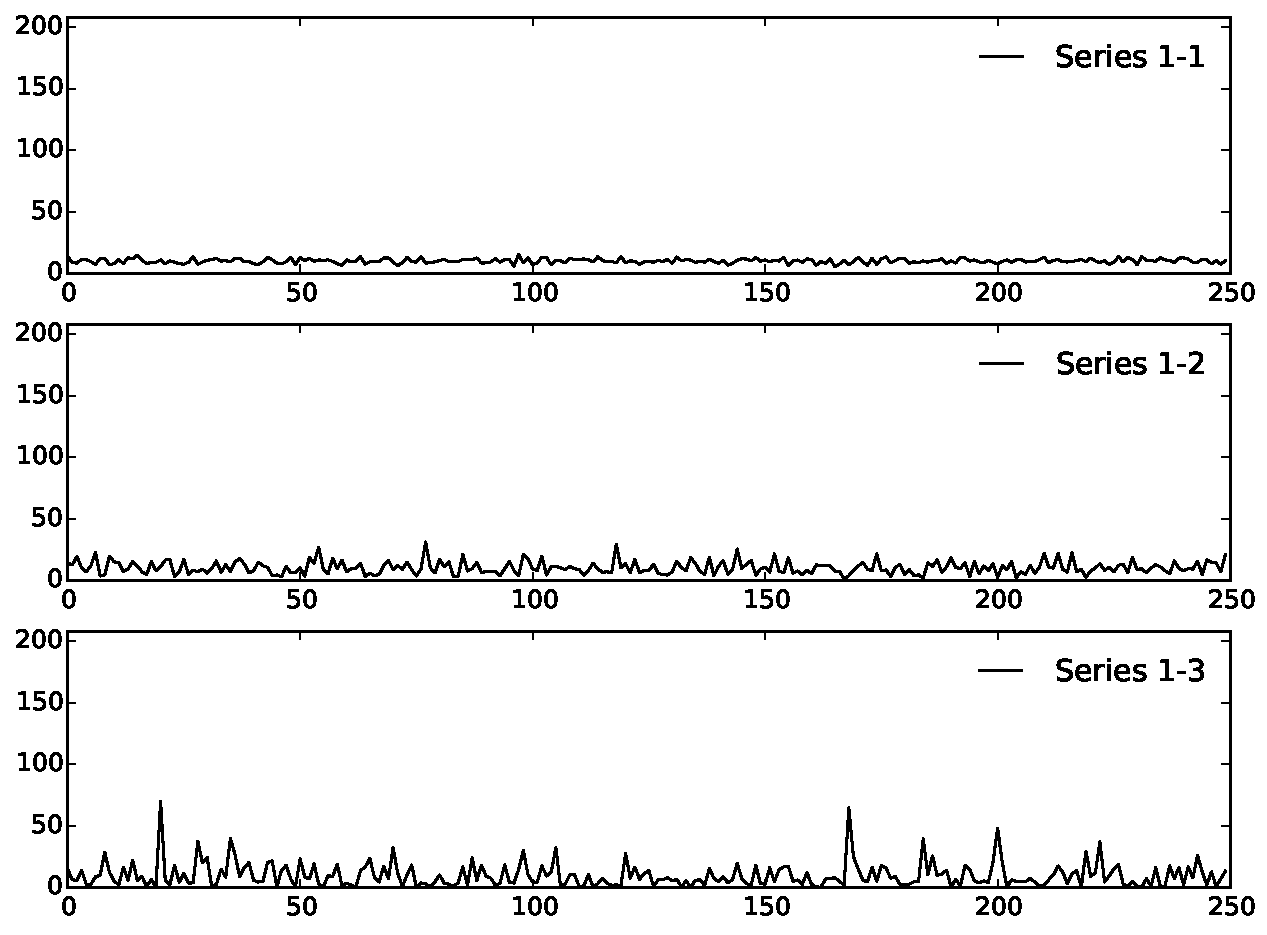
\includegraphics[width=.4\linewidth]{figures/Patterns_1.pdf}
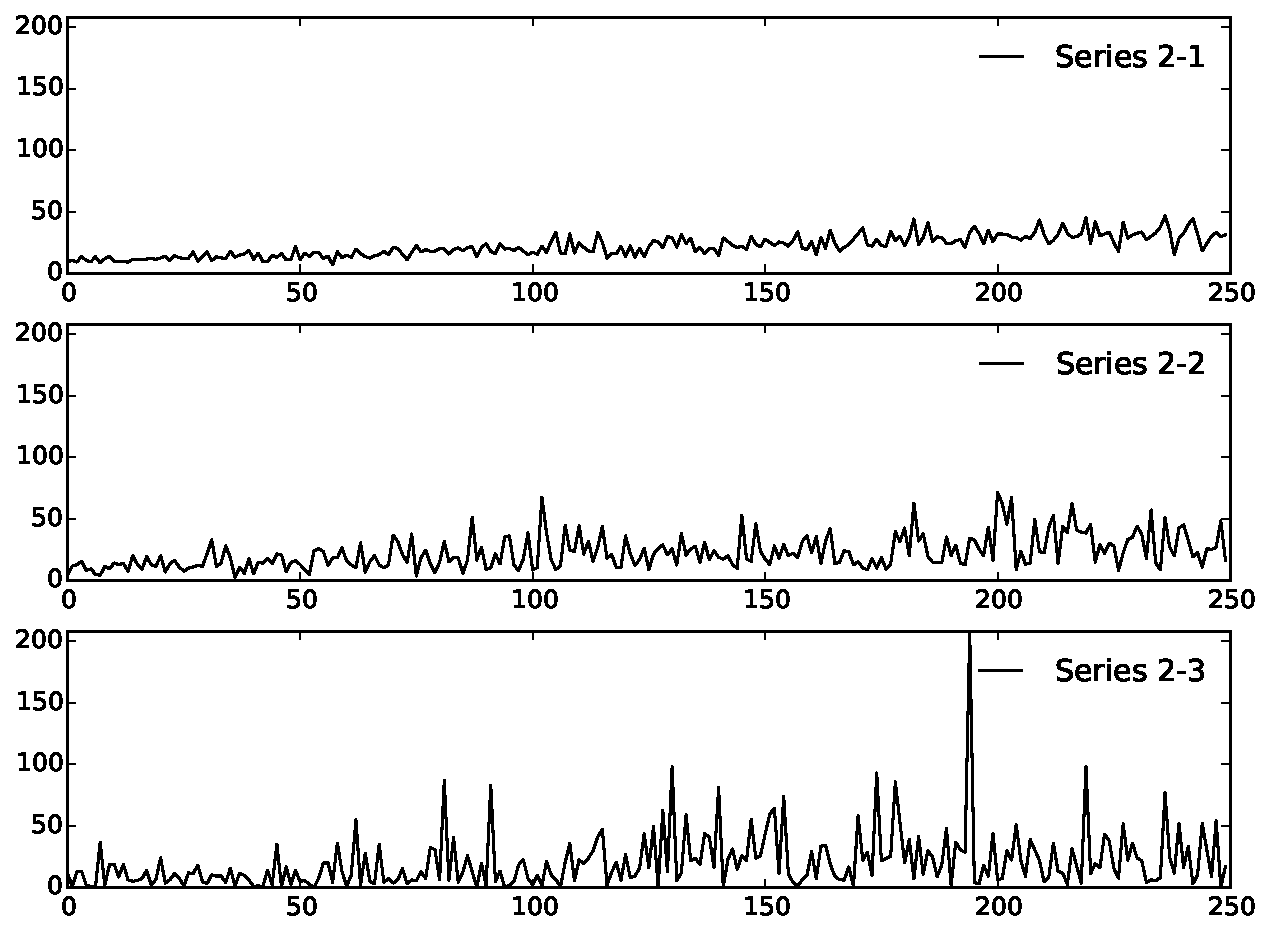
\includegraphics[width=.4\linewidth]{figures/Patterns_2.pdf} \\
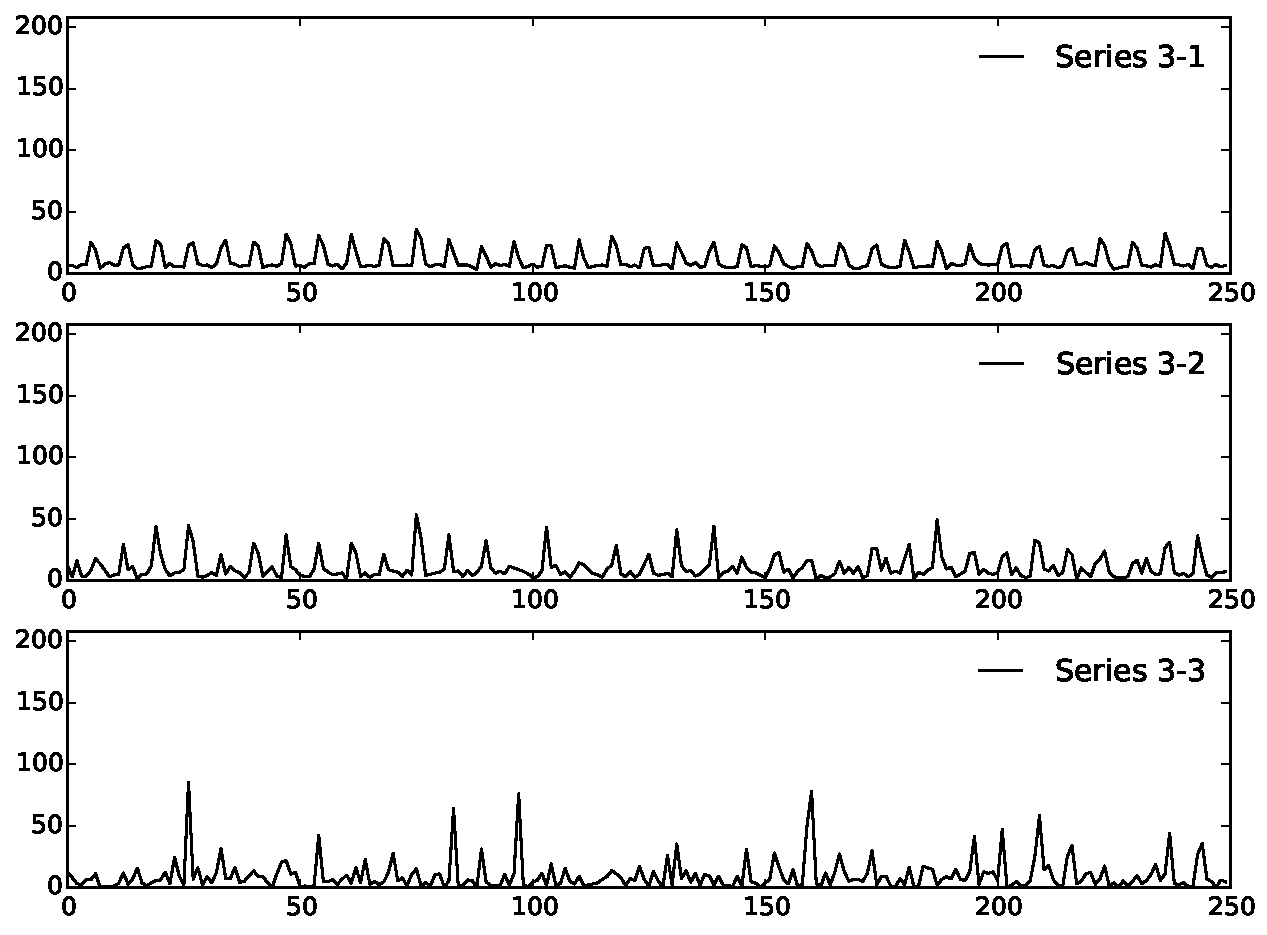
\includegraphics[width=.4\linewidth]{figures/Patterns_3.pdf}
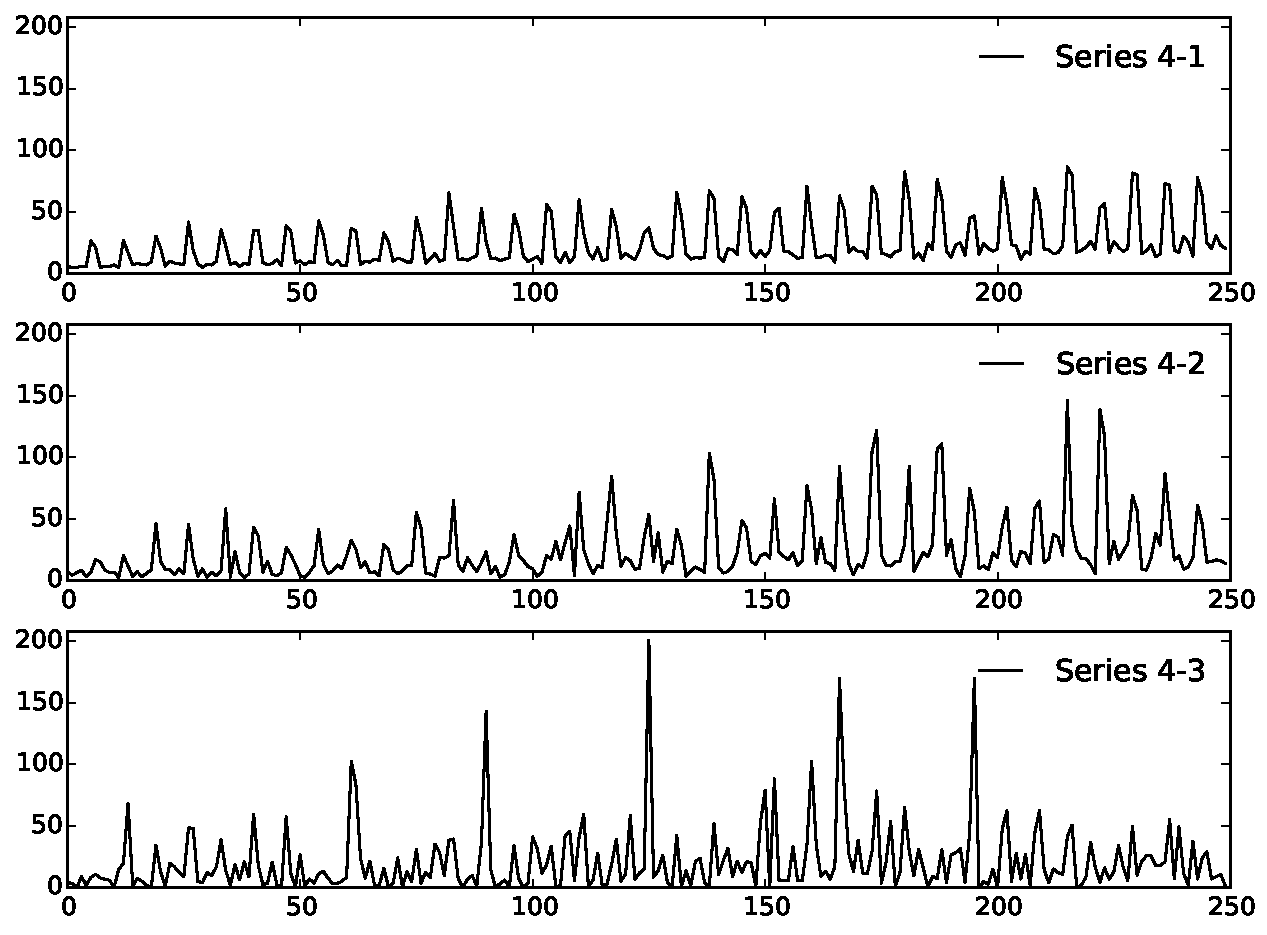
\includegraphics[width=.4\linewidth]{figures/Patterns_4.pdf}
\caption{Exercise~\ref{plots} plots}
\label{fig:plots}
\end{figure}
\end{landscape}
\newpage

%\begin{landscape}
%\let\thefootnote\relax\footnotetext{\textbf{Question~\ref{inter}}}
%
%\begin{center}
%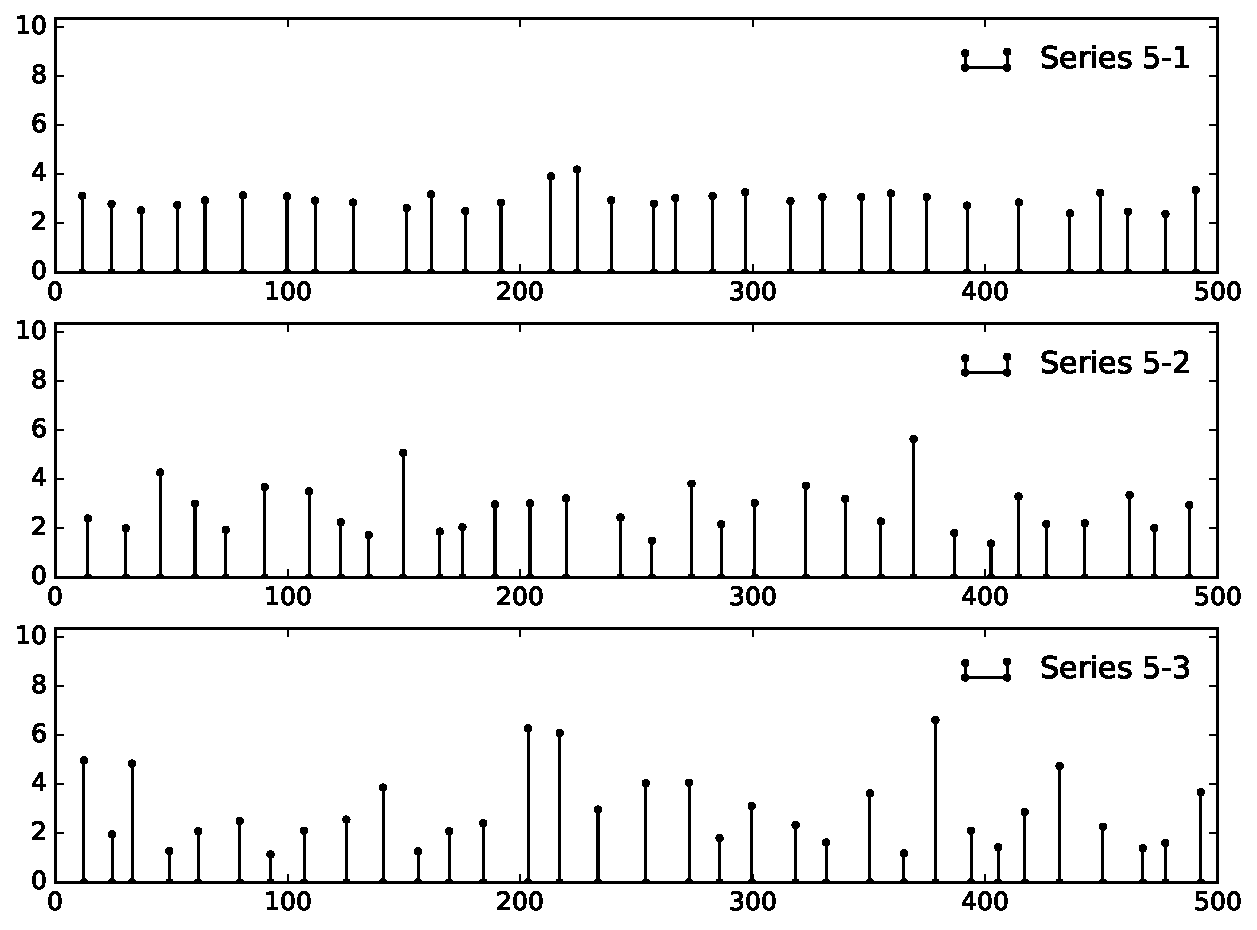
\includegraphics[width=.49\linewidth]{figures/Intermittent_1.pdf}
%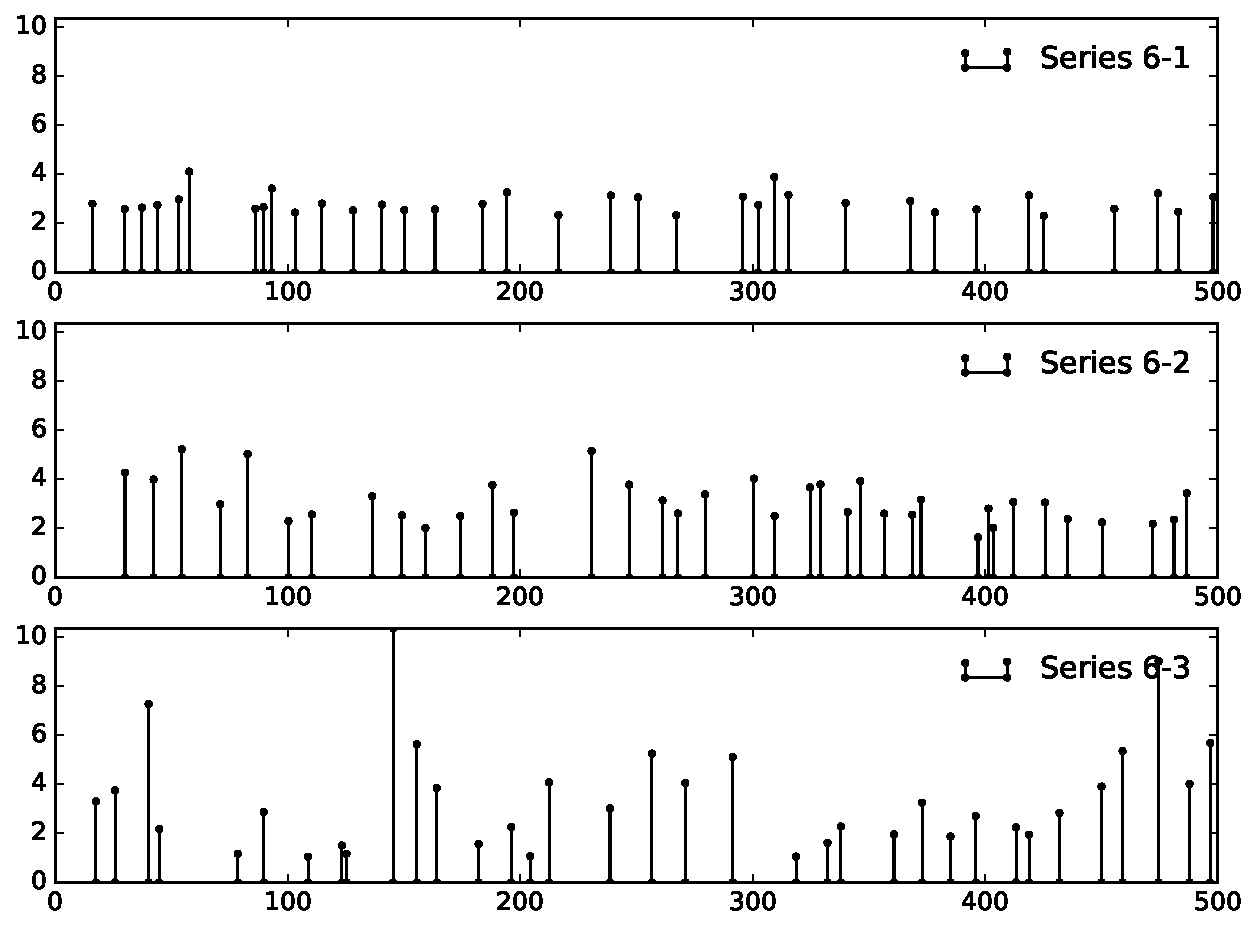
\includegraphics[width=.49\linewidth]{figures/Intermittent_2.pdf} \\
%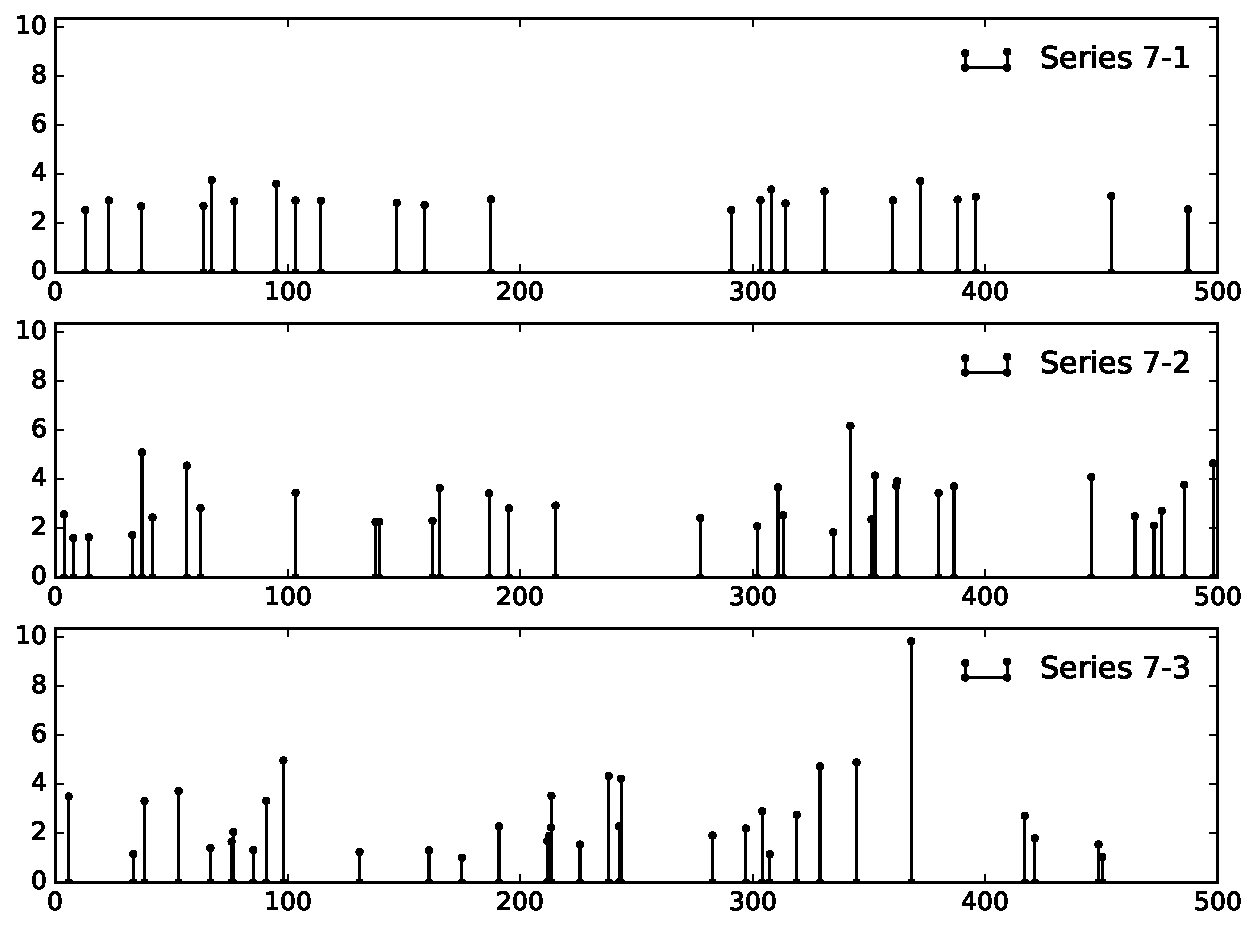
\includegraphics[width=.49\linewidth]{figures/Intermittent_3.pdf}
%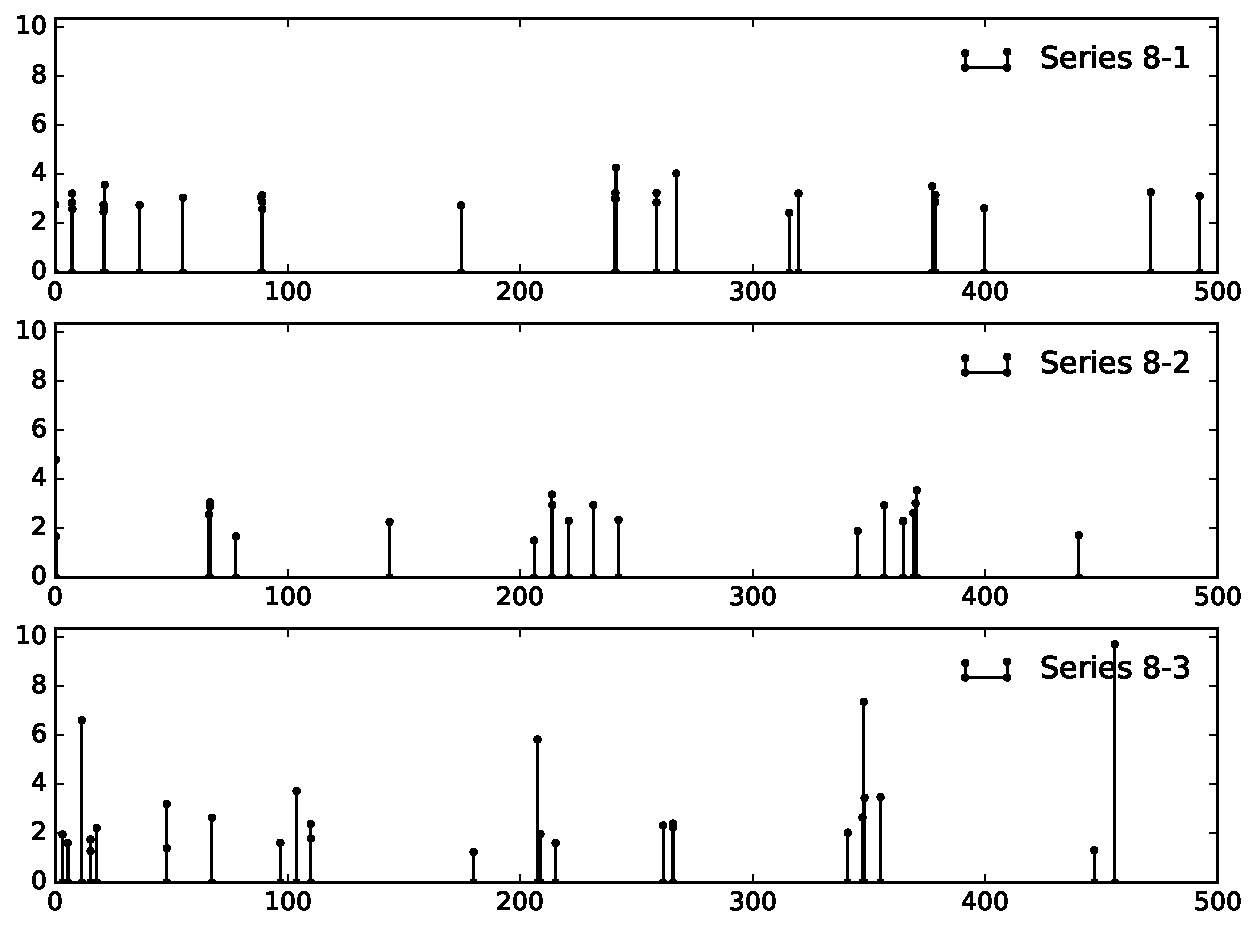
\includegraphics[width=.49\linewidth]{figures/Intermittent_4.pdf}
%\end{center}
%\end{landscape}





%\begin{question}
%The EOQ model is based on the assumption that the fixed ordering cost is independent of the order quantity. Consider the following variant of the model where this assumption is not valid anymore. Here, if the order quantity is less than or equal to $Q^{\max}$, then the fixed ordering cost will be $A_1$, and it will be $A_2$ otherwise. 
%
%\begin{enumerate}
%\item Develop a procedure to find the optimal order quantity for this variant of the EOQ model.
%\item Assume that the demand $D$ that is used in computing the order quantity is off by a factor of $\Delta$. That is, actual demand happens to be $D(1+\Delta)$ rather than $D$. 
%
%\end{enumerate}
%
%We have the following data: $A_1=50$, $A_2=85$, $Q^{\max}=100$, $h=2$, $D=1000$. 
%
%
%(for the sake of simplicity neglect the unit production cost)
%
%Now assume that the demand $D$ that is used in computing the order quantity is off by a factor of $\Delta$. That is, actual demand happens to be $D(1+\Delta)$ rather than $D$. 
%
%  \begin{solution}
%TBD
%
%\begin{center}
%\includegraphics[width=.5\linewidth]{figure_2.pdf}
%\end{center}
%  \end{solution}
%\end{question}




%
%
%Forecast approaches
%Extrapolation of historical data
%• Time series
%• Regression
%• Smoothing
%• Forecasts based on other factors
%• Promotions
%• Substitution effects
%• Dependent items (MRP)
%• Economic conditions
%• Expert knowledge
%
%
%Phases in identifying and using a forecasting model
%1. Pattern recognition (level, trend, season, shift)
%2. Factor initialization (level, trend factor, seasonal effect)
%3. Select time series forecasting model (e.g., mov. average, exp sm.)
%4. Develop forecasting model over time by updating factors (level,
%trend, season) after new data has become available
%5. Optimize forecasting parameters (n,α,β,γ) using criterion (e.g.,
%MSE or MAPE) based on subset of data
%6. Test forecasting model on complete dataset (i.e., are the errors
%independently normally distributed –you are ready-or did we miss a
%pattern –return to 1-?)





%Lead time
%› What lead time to use in our models?
% Lead time from supplier to inventory?
% Lead time from inventory to customer?
%› How to express lead times?
% Working days?
% Calendar days?
% Days, Weeks, Months, Years?
%
%How to model lead times?
% Constant or zero
% Dynamically varying (e.g. seasonal patterns)
% Stochastically varying (beware of crossovers)
%
%lead time in inventory models:
%the time between
%the moment a decision is made to issue an order
%and
%the first moment when a not-yet issued order is
%available for service to the customer
%
%
%Continuous and Periodic Review
%and Review period R: Risk period
%Length of time between successive observations
%of the inventory position (=“can order” moments)
%Continuous inventory control: R=0
%Periodic inventory control: R>0
%Is the review period included in the lead time?
%
%
%Review period and Risk period
%The current order should cover demand +
%uncertainty up till earliest arrival of next order:
%If R=0: Next order moment when demand occurs
%Risk period = L
%If R>0: Next order moment after R periods
%Risk period = L+R
%“Lead time demand”=demand during the Risk period
%
%Lead time demand distribution
%Risk period demand distribution
%› Text book approach:
%› Convolution of
% constant lead time (risk period) L
% stationary independent demand distribution
%- stationary means: no trends, no seasons
%- independent means: demand in one period
%does not depend on demand in other periods
%- constant mean μ, standard deviation σ / period
% Lead time demand ~(L*μ; σ√L)
%
%
%Lead time demand distribution
%Risk period demand distribution
%› Problems:
% Are risk periods constant?
% Is demand per period stationary?
% Is demand information per period independent?
%› Solutions:
% Model uncertainty in lead times/risk periods
% Use stationary forecast errors per period
% Forecast for whole lead time (risk period) ahead
%
%
%Lead time demand distribution
%Risk period demand distribution
%› Use of forecast and forecast error in
%non─stationary demand distribution
%› If forecasting has resulted in normal distributed
%forecast error:
% Use forecast next period as estimator of the
%expected demand in that period
% Use Root Mean Squared Error as initial estimator
%of the standard deviation of the expected demand
% Correct standard deviation based on lead time
%length and smoothing parameter used
%
%
%Lead time demand distribution
%Risk period demand distribution
%› Forecasting may NOT result in normal
%distributed forecast error if:
% Number of observations is too small (<30)
% Mean demand per period is too small (<10)
% Coefficient of variation (σ/μ) > 0.5
%› Other lead time demand distributions:
% Poisson (discrete distribution if demand < 10)
% Lognormal or Gamma (avoid negatives)
% Bootstrapping (sampling from original data)
%
%
%Service levels
%How to measure service of an inventory system?
%› Service to whom?
%› Service from where?
%› Service time limited?
%› Partial deliveries?
%› Differences in service over time?
%
%Two inventory control service levels measure
%differences in service over time.
%› P1: Service level per cycle
%› P2: Fill Rate
%
%P1: Service level per cycle
%Cycle starts when Q arrives
%Cycle ends when next Q arrives
%Frequency of stockout
%at the end of a cycle
%How many cycles for
%good measure?
%
%
%P2: Service level: Fill Rate
%% demand that can be fulfilled from stock
%30
%P1
%P2
%• Better relation with
%experienced service
%by customer
%• Easier to show trend
%in service over time
%• Lower safety stock
%required
%• Calculations more
%complex
%|
%
%Summary
%› Coping with intermittent demand
%› Focus on time horizon for which we need forecasts
% Lead time
% Review Period
%› What to do if forecast errors are not normal, but
%no further patterns to be included in model?
%› What service level is appropriate?





%\section{Week 3 of Jan's lecture}
%\label{sec:week-3-jans}
%
%
%
%Inventory points, Lead times, I/O interface
%• Inventory Control Models
%• Objective
%• Decision Variables
%• Constraints
%• Parameters
%• Assumptions
%• Periodic review or continuous review
%• Other models
%• Calculating P1 and P2 service level
%
%
%There are typically mutliple inventory points to consider
%\begin{itemize}
%\item From supplier to RMI
%\item From RMI to CODP
%\item From CODP to FGI
%\item From FGI to customer
%\end{itemize}
%make clear what lead time you consider
%
%How to control the lead time ..
% to the customer?
% from RMI to the CODP?
% from the supplier to the RMI?
%
%› If we would like to control inventory, we …
% choose a specific inventory point to control
% take decisions that affect the inventory at
%that point
% know how to measure the effectiveness of
%these decisions
%
%Inventory control
%What about the
%• Objective
%• Decision Variables
%• Constraints
%• Parameters
%• Assumptions
%
%
%
%Inventory Control
%What about uncertainty?
%• What parameters?
%• How to model?
%• Ignore
%• Include
%
%me
%› Continuous review (Q,r) model: order Q if IP≤r
% R
%R+Q
%L L
%Inventory position
%Inventory level
%Time
%SS
%0
%W
%
%\section{Week 4}
%\label{sec:week-4}
%
%ABC classification (Teunter et al., 2010)
%• Service level optimisation (Teunter et al., 2010)
%• Multi-item problems
%• Commonality (Baker et al., 1986)
%• Perishability
%
%ABC according to APICS
%ABC classifies a group of SKUs in
%decreasing order of annual dollar volume
%(price multiplied by projected volume) or
%other criteria. This array is then split into
%three classes, called A, B and C.
%(Blackstone and Cox, 2008)
%
%The standard practice is to assign the same
%service level to each SKU in a particular class
%Lee - NONSTOP solutions
%Pflitsch - SLIMSTOCK
%
%Which class should get the highest service level?
%› Some authors have argued that A items are
%the most critical for a firm.
%› Others have claimed that dealing with
%stockouts is not worth the effort for C items.
%Hopp \& Spearman:
%It makes sense to use sophisticated time-consuming techniques to
%tightly coordinate the arrival of A-parts, not for C-items.
%Slack et al.:
%Different inventory management decision rules are needed for
%different classes of inventory
%
%Service Level P2 – Fill Rate
%› The fill rate (FR) is the fraction / percentage of
%customers satisfied directly from stock on hand.
%› It is the most widely applied service level measure.
%› Although the calculations to find k are more
%complex, the good news is that software can do this!
%› But software does not tell you what an appropriate
%fill rate is and whether it should be the same for
%every SKU!
%
%Multiple items
%Service levels for demand for multiple items:
%Volume Fill rate = fraction of demanded units
%available from stock on hand
%Or
%Order line Fill rate = fraction of order lines
%that are completely available from stock on
%hand
%Or
%Order Fill rate = fraction of orders completely
%available from stock on hand





%%% Local Variables:
%%% mode: latex
%%% TeX-master: "notes_all"
%%% End:


\section{Choosing Inventory Policies}
% \subsection{Variations on the EOQ model}
\label{sec:variations-eoq-model}

\begin{question}
  When choosing an inventory policy, i.e., a policy that decides when
  and how much to order, we need to understand the environment first
  in which the policy is going to operate. Can you use
  Question~\ref{ex:1} to come up with a characterization of the environment? 
  \begin{solution}
    A simple starting point is provided by this table.
    \begin{table}[h]
      \centering
    \begin{tabular}{l|l|l|l}
      Environment && &  \\ \hline
Demand & variability &deterministic/constant & Stochastic \\ 
& substitution effects & yes & no \\
\hline Supply & Lead time & $L=0$& $L>0$ \\ 
& perishable items & yes & no\\
& Joint ordering & yes & no\\
& Order size constraints &yes & no \\
\hline Cost structure &Ordering cost & $A=0$ & $A>0$ \\ 
& holding cost & $h=0$ &$h>0$ \\
& fixed backlog cost & $\pi=0$ &$\pi>0$\\
&variable backlog cost & $b=0$ &$b>0$\\
&lost sales cost &$k=0$ & $k>0$ \\
&quantity discounts &yes & no \\
\hline KPIs &fill rate $S$ & yes & no\\ 
& cycle service level &yes& no\\
    \end{tabular}
    \caption{(Incomplete) characterization of the environment of inventory policies}
      \label{tab:environment}
    \end{table}
  \end{solution}
\end{question}

\begin{question}
  Characterize the EOQ model by means of the table of the previous
  question.
  \begin{solution}
    \begin{table}[h]
      \centering
    \begin{tabular}{l|l|l|l}
      Environment && &  \\ \hline
Demand & variability &\boxed{deterministic/constant} & Stochastic \\ 
& substitution effects & yes & \boxed{no} \\
\hline Supply & Lead time & \boxed{$L=0$}& $L>0$ \\ 
& perishable items & yes & \boxed{no}\\
& Joint ordering & yes & \boxed{no}\\
& Order size constraints &yes & \boxed{no} \\
\hline Cost structure &Ordering cost & $A=0$ & $\boxed{A>0}$ \\ 
& holding cost & $h=0$ & $\boxed{h>0}$ \\
& fixed backlog cost & $\pi=0$ & $\boxed{\pi=\infty}$\\
&variable backlog cost & $b=0$ &$\boxed{b=\infty}$\\
&lost sales cost &$k=0$ & $\boxed{k=\infty}$ \\
&quantity discounts &yes & \boxed{no} \\
\hline KPIs &fill rate & $\boxed{S=1}$ & no\\ 
& cycle service level &yes& no\\
    \end{tabular}
    \caption{EOQ model }
      \label{tab:environment}
    \end{table}
  \end{solution}
\end{question}

\begin{question}
  In the next set of questions we are going to modify the assumptions
  of the EOQ model with the aim to investigate how the environment
  affects the inventory policy. For the sake of comparison, sketch how the inventory behaves over time for the EOQ model and write down the cost function.

  \begin{solution}
\begin{center}
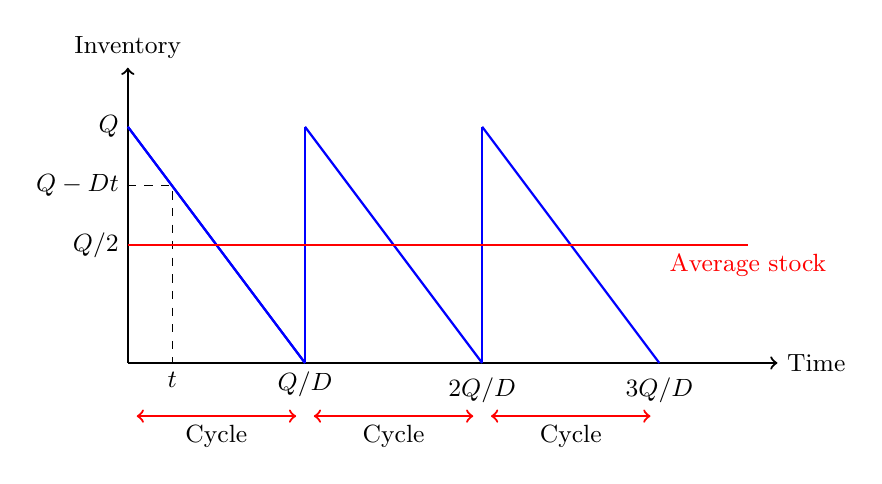
\begin{tikzpicture}[x=0.75cm,y=0.015cm]
\small
\draw[thick,->] (0,0) -- (11,0) node[right] {Time};
\draw[thick,->] (0,0) -- (0,250) node[above] {Inventory};
\draw[] (0,200) node[left] {$Q$};
\draw[color=blue,thick] (0,200) -- (3,0);
\draw[] (0.75,0) node[below] {$t$};
\draw[] (0,150) node[left] {$Q-Dt$};
\draw[dashed] (0,150) -- (0.75,150) -- (0.75,0);
\draw[] (3,0) node[below] {$Q / D$};
\foreach \y in {1,...,3}{
	\draw[color=blue,thick] (3*\y-3,200) -- (3*\y,0);}
\foreach \y in {1,2}{
	\draw[color=blue,thick] (3*\y,0) -- (3*\y,200);}
\foreach \y in {2,3}{
	\draw[] (3*\y,-5) node[below] {\y $Q/D$};}
\draw[] (0,100) node[left] {$Q / 2$};
\draw[color=red,thick] (0,100) -- (10.5,100) node[below] {Average stock};
\foreach \y in {0,...,2}{
	\draw[color=red,thick,<->] (3*\y+0.15,-45) -- (3*\y+3-0.15,-45);
	\draw[] (3*\y+1.5,-45) node[below] {Cycle};}
\end{tikzpicture}
\end{center}

The total cost for one cycle is the order cost plus the inventory cost. The order cost is $A$, the inventory cost is the total area of the triangle times $h$, i.e. 
\begin{equation*}
  \frac h2\text{height}\cdot\text{base} = \frac h 2 Q\cdot \frac QD= \frac h2 \frac{Q^2}D.
\end{equation*}
The average cost per unit time is this total cost divided by the duration of one cycle, which is $Q/D$. Therefore, the average cost is
\begin{equation*}
\frac A{Q/D}+  \frac{ h/2 \cdot Q^2/D}{Q/D} = \frac h 2 \frac {Q^2} D\cdot \frac D/Q = \frac D Q A + \frac h2 Q.
\end{equation*}

\begin{center}
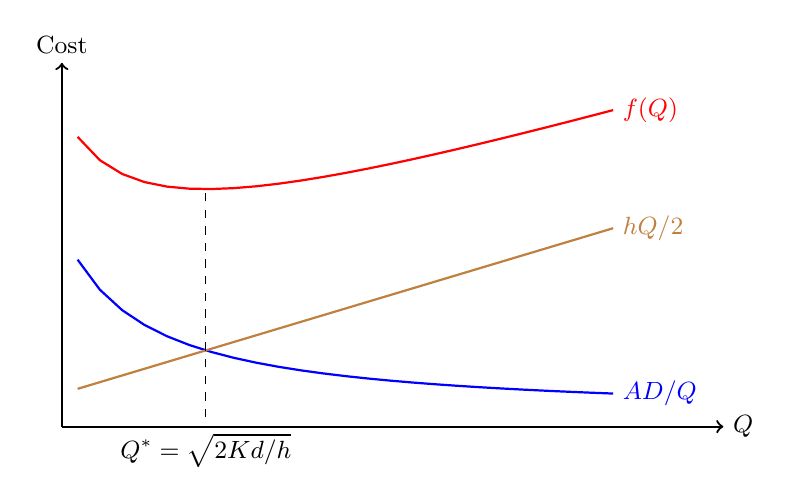
\begin{tikzpicture}[x=0.02cm,y=0.06cm]
\small
\def\c{1} 
\def\K{100} 
\def\h{0.2} 
\def\d{20} 
\pgfmathsetmacro{\Q}{sqrt(2)*sqrt(\K)*sqrt(\d)/sqrt(\h)}
\pgfmathsetmacro{\f}{sqrt(2)*sqrt(\K)*sqrt(\d)*sqrt(\h)+\c*\d}	
\draw[thick,->] (50,-2) -- (470,-2) node[right] {$Q$};
\draw[thick,->] (50,-2) -- (50,75) node[above] {Cost};
\draw[color=blue,thick,domain=60:400] plot (\x,{\d*\K/\x}) node[right] {$AD / Q$};
\draw[color=brown,thick,domain=60:400] plot (\x,{\h*\x/2}) node[right] {$hQ / 2$};
\draw[color=red,thick,domain=60:400] plot (\x,{\d*\K/\x+\c*\d+\h*\x/2}) node[right] {$f(Q)$};
\draw (\Q,-1.5) node[below] {$Q^{*} = \sqrt{2Kd / h}$};
\draw[dashed] (\Q,0) -- (\Q,\f);
\end{tikzpicture}
\end{center}

  \end{solution}
\end{question}

\begin{question}
  It is very important to memorize that the total inventory cost for
  the EOQ model is quite insensitive to the actual order quantity
  $Q$. Show this for the case with $A=100$, $h=0.2$, and $D=20$. What
  happens to the total cost if $Q=60, 80, \ldots 200$?
  \begin{solution}
From the EOQ formula
\begin{itemize}
\item $Q^{*} \approx 141.42$ units
\item $f(Q^{*}) \approx \mathdollar 48.28$
\end{itemize}

\begin{center}
\footnotesize
\begin{tabular}{rrrrr}
\toprule
$Q$     & $AD/Q$  &  $hQ/2$  & $f(Q)$ \\
\midrule
    60    & 33.33 &  6.00  & 59.33 \\
    80    & 25.00 &  8.00  & 53.00 \\
    100   & 20.00 &  10.00 & 50.00 \\
    120   & 16.67 &  12.00 & 48.67 \\
    140   & 14.29 &  14.00 & 48.29 \\
    160   & 12.50 &  16.00 & 48.50 \\
    180   & 11.11 &  18.00 & 49.11 \\
    200   & 10.00 &  20.00 & 50.00 \\
\bottomrule
\end{tabular}
\end{center}
  \end{solution}
\end{question}

\begin{question}
  As a first variation, what would you change/do if the lead time $L$
  is no longer 0, but becomes positive? (Thus, all the other
  assumptions of the EOQ model stay the same, only the lead time
  becomes positive.)  In other words, how would you change the EOQ
  policy, and determine when and how to order?
  \begin{solution}
    Since the backlog costs are infinite, backlogging is not
    desirable, hence we order early. See the graph: 
\begin{center}
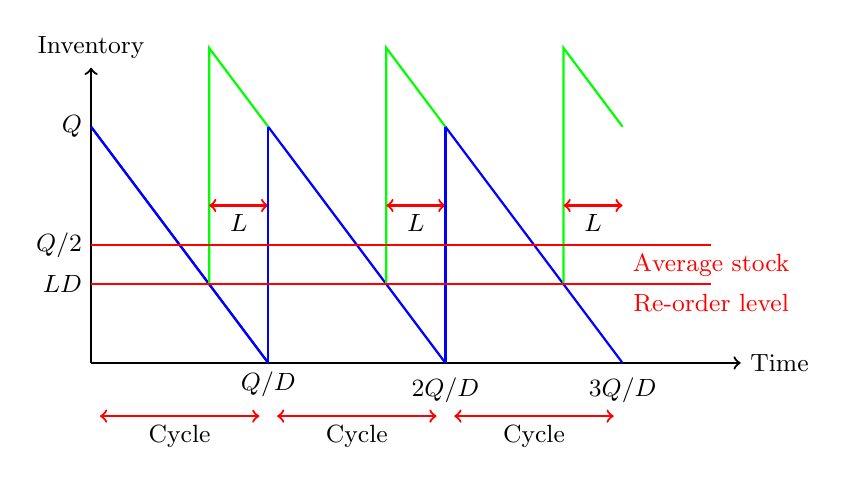
\begin{tikzpicture}[x=0.75cm,y=0.015cm]
\small
\draw[thick,->] (0,0) -- (11,0) node[right] {Time};
\draw[thick,->] (0,0) -- (0,250) node[above] {Inventory};
\draw[] (0,200) -- (0,200) node[left] {$Q$};
\draw[color=blue,thick] (0,200) -- (3,0);
\draw[] (3,0) node[below] {$Q / D$};
\foreach \y in {1,...,3}{
	\draw[color=blue,thick] (3*\y-3,200) -- (3*\y,0);
	\draw[color=green,thick] (3*\y-3+2,200/3) -- (3*\y-3+2,200/3*4) -- (3*\y,200);
	\draw[color=red,thick,<->] (3*\y-3+2,200/3*2) -- (3*\y,200/3*2);
	\draw[] (3*\y-3+2.5,200/3*2) node[below] {$L$};}
\foreach \y in {1,2}{
	\draw[color=blue,thick] (3*\y,0) -- (3*\y,200);}
\foreach \y in {2,3}{
	\draw[] (3*\y,-5) node[below] {\y $Q/D$};}
\draw[] (0,100) node[left] {$Q / 2$};
\draw[color=red,thick] (0,100) -- (10.5,100) node[below] {Average stock};
\draw[] (0,200/3) node[left] {$L D$};
\draw[color=red,thick] (0,200/3) -- (10.5,200/3) node[below] {Re-order level};
\foreach \y in {0,...,2}{
	\draw[color=red,thick,<->] (3*\y+0.15,-45) -- (3*\y+3-0.15,-45);
	\draw[] (3*\y+1.5,-45) -- (3*\y+1.5,-45) node[below] {Cycle};}
\end{tikzpicture}
\end{center}
    
This new policy can be described in a simple way by introducing the
concept of \emph{inventory position}, that is, all stock on-hand plus
the replenishments under way. The green graph above illustrates the
inventory position $IP$. When $IP$ hits the lead time demand $L D$,
i.e., the lead time $L$ times the demand $D$, we should order
$Q$. During the lead time $L$ the demand will be met from on-hand
stock. When the replenishment arrives a lead time $L$ later, it
arrives just in time to meet the demand again .
  \end{solution}
\end{question}

\begin{question}

How can we decompose leadtime?

\begin{solution}
TBD
\end{solution}

\end{question}



\begin{question}
  What would happen if it is allowed to backorder demand, in other
  words $b>0$, but $\pi = 0$? (We set $L=0$ again.)
  \begin{solution}
\begin{center}
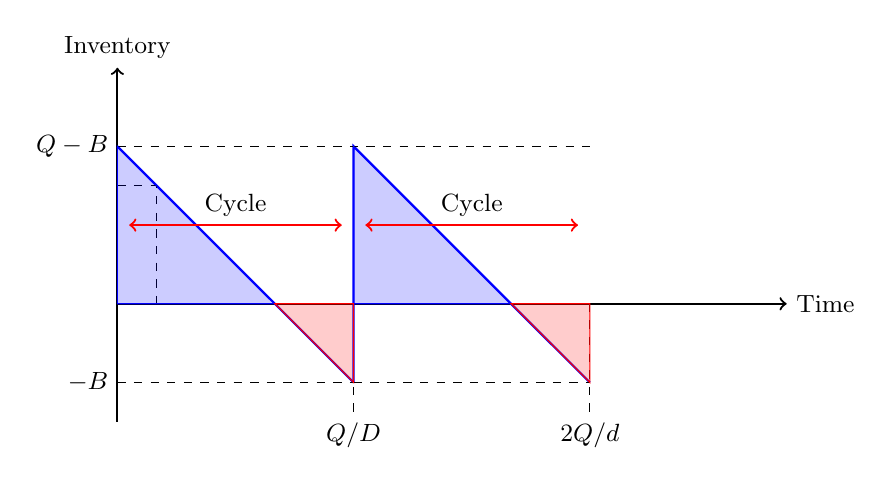
\begin{tikzpicture}[x=1cm,y=0.01cm]
\small

\draw[thick,->] (0,0) -- (8.5,0) node[right] {Time};
\draw[thick,->] (0,-150) -- (0,300) node[above] {Inventory};

\draw[] (0,200) node[left] {$Q - B$};

\draw[color=blue,thick] (0,200) -- (3,-100);

\draw[] (0,-100) node[left] {$-B$};
\draw[dashed] (0,-100) -- (3,-100);

%\draw[] (0,150) node[left] {$Q - B - Dt$};
%\draw[] (0.5,0) node[below] {$t$};
\draw[dashed] (0,150) -- (0.5,150) -- (0.5,0);

%\draw[] (2,0) node[below] {$(Q - B) / d$};

\draw[dashed] (3,0) -- (3,-140) node[below] {$Q / D$};

\draw[color=blue,thick] (3,-100) -- (3,200) -- (6,-100);
%\draw[] (5,0) node[below] {$(2Q - B) / d$};
\draw[dashed] (6,0) -- (6,-140) node[below] {$2Q / d$};
\draw[dashed] (0,200) -- (6,200);
\draw[dashed] (3,-100) -- (6,-100);

\draw [draw=blue,fill=blue,fill opacity=0.2] (0,0) -- (0,200) -- (2,0) -- cycle;
\draw [draw=blue,fill=blue,fill opacity=0.2] (3,0) -- (3,200) -- (5,0) -- cycle;
\draw [draw=red,fill=red,fill opacity=0.2] (2,0) -- (3,-100) -- (3,0) -- cycle;
\draw [draw=red,fill=red,fill opacity=0.2] (5,0) -- (6,-100) -- (6,0) -- cycle;

\foreach \y in {0,1}{
	\draw[color=red,thick,<->] (3*\y+0.15,100) -- (3*\y+3-0.15,100);
	\draw[] (3*\y+1.5,100) node[above] {Cycle};}
\end{tikzpicture}
\end{center}

The blue area is
\begin{equation*}
\frac12  \text{height}\cdot\text{base} = \frac12 (Q-B)\frac{(Q-B)}{D}=\frac{(Q-B)^2}{2D}
\end{equation*}
while the red area is
\begin{equation*}
  \frac12 B \frac{B}{D}=\frac{B^2}{2D}.
\end{equation*}
Thus, the time average cost is the total cost divided by the cycle lenght $Q/D$:
\begin{equation*}
  \begin{split}
  F(Q) 
&= \frac{D}{Q}A + \frac{h(Q-B)^2/2D}{Q/D} + \frac{b B^2/2D}{Q/D} \\
&= \frac{D}{Q}A + h\frac{(Q-B)^2}{2Q} + b \frac{B^2}{2Q}.
  \end{split}
\end{equation*}
Check that by setting $B=0$ you get the old EOQ result.
\end{solution}
\end{question}

\begin{question}
  What happens to the optimal cost if you allow for backorders?  What
  will happen to the optimal order quantity $Q$, will it become larger or smaller? 
  \begin{solution}
    The cost must become lower, since we remove a constraint. 

    Let's see by how much.  This is not so simple, however, because we
    now have two `controls' (or degrees of freedom): the order
    quantity $Q$ and the backorder level $B$. Even though it is
    possible to find a closed form solution for the optimal values of
    $Q$ and $B$, here we satisfy ourselves with a graphical analysis.
    We are going to make a plot of the total cost as a function of $Q$
    for various values of $B$.

    Here is an example. Take $A=100$, $h=0.2$, $D=20$, $B=10$, $b=1$.

\begin{center}
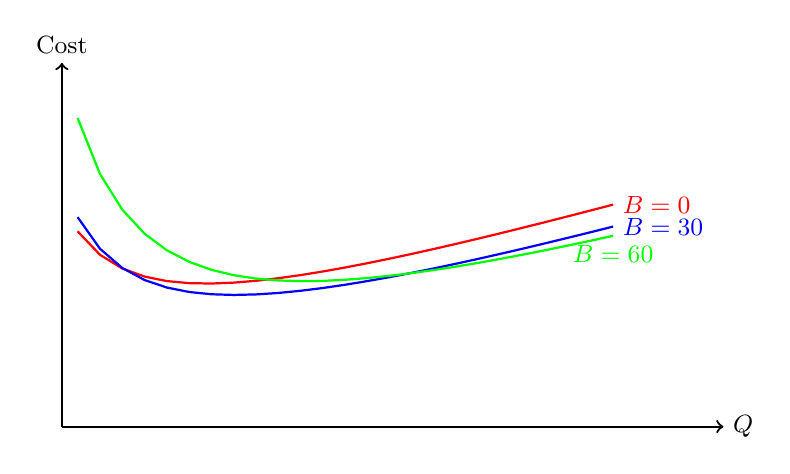
\begin{tikzpicture}[x=0.02cm,y=0.06cm,
declare function = {
f(\Q) = \D*\A/\Q+\h/2*(\Q-\B)/\Q*(\Q-\B)+\b/2*\B/\Q*\B; }
]
\small
\def\A{100} 
\def\h{0.2} 
\def\D{20} 
\def\b{1}
%\def\B{0}
%\pgfmathsetmacro{\f}{sqrt(2)*sqrt(\A)*sqrt(\D)*sqrt(\h)}	
\draw[thick,->] (50,-2) -- (470,-2) node[right] {$Q$};
\draw[thick,->] (50,-2) -- (50,75) node[above] {Cost};
%\draw[color=red,thick,domain=60:400] plot function{\D*\A/x+\h*x/2} node[right] {$B=0$};
%\draw[color=red,thick,domain=60:400] plot (\x,{\D*\A/\x+1*pow(\x,2)}) node[right] {$B=0$};
\def\B{0}
\draw[color=red,thick,domain=60:400] plot (\x,{f(\x)}) node[right] {$B=\B$};
\def\B{30}
\draw[color=blue,thick,domain=60:400] plot (\x,{f(\x)}) node[right] {$B=\B$};
\def\B{60}
\draw[color=green,thick,domain=60:400] plot (\x,{f(\x)}) node[below] {$B=\B$};
% \begin{axis}
% \addplot {f(x)};
% \end{axis}
\end{tikzpicture}
\end{center}


We see that the curve related to $B=30$, i.e., the
blue curve, achieves the lowest point of each of the three graphs.
The minimum of the blue curve is realized a bit to the right of the
minimum of the $B=0$ curve, i.e., the red curve.  Thus, from the
graphs, by setting $B=30$ and $Q$ a bit larger than the optimal value
for the EOQ model, we can lower the cost a bit.

% \begin{tikzpicture}[domain=-1:1,yscale=2,xscale=4,smooth]
% %\fill[gray] (-1.2,-1.2) rectangle (1.2,2.5);
% \draw[very thin] (-1.1,-1.1) grid[step=.5] (1.1,2.4);
% \draw[thick,->] (-1.2,0) -- (1.2,0);
% \draw[thick,->] (0,-1.2) -- (0,2.5);
% \draw[color=red] plot[id=1] function{cos(pi*x)};
% \draw[color=blue,thick] plot[id=2] function{cos(pi*x)+cos(2*pi*x)/2};
% \draw[color=green!50!black,thick] plot[id=3] function{cos(pi*x) + cos(2*pi*x)/2 + cos(3*pi*x)/3};
% \draw[color=yellow,thick] plot[id=4] function{cos(pi*x) + cos(2*pi*x)/2 + cos(3*pi*x)/3 + cos(4*pi*x)/4};
% %\draw<5->[color=cyan,thick] plot[id=5] function{cos(pi*x) + cos(2*pi*x)/2 + cos(3*pi*x)/3 + cos(4*pi*x)/4 + cos(5*pi*x)/5};
% \end{tikzpicture}

% \begin{tikzpicture}[
% declare function={ Nprime(\x)                 = 1/(sqrt(2*pi))*exp(-0.5*(pow(\x,2))); 
%                    d2(\x,\y,\KK,\RR,\SIG)     = (ln(\x/\KK)+(\RR-(pow(\SIG,2)/2)*\y))/(\SIG*(sqrt(\y)));
%                    myfun(\x,\y,\KK,\RR,\SIG)  = exp(-\RR*\y)*Nprime(d2(\x,\y,\KK,\RR,\SIG))/(\x*\SIG*sqrt(\y));
%                  },
% ]
% \begin{axis}[y domain=0.01:0.3,domain=95:105,view={150}{20}]
% \addplot3[surf] {myfun(x,y,100,0,0.09)};
% \end{axis}
% \end{tikzpicture}

  \end{solution}
\end{question}

\begin{question}
  What would you do if $b=0$, $\pi > 0$ and $h>0$? 
  \begin{solution}

TBD. 
    We have two alternatives. If we decide to keep no inventory, we
    only have to pay for backlogging demand. 

    Demand needs to enter in discrete amounts, for otherwise paying
    $\pi$ per demand becomes a bit strange.
  \end{solution}
\end{question}

\begin{question}We can also decide to reject demand rather than
  backlog it. Can you sketch the consequences on the behavior of the
  inventory level?  What happens to the order quantity $Q$?  What are
  the consequences in terms of cost, does it become lower or higher?
  \begin{solution}
    The influence on the cost is qualitatively easy. Once again we
    relax a constraint, hence it must be possible to reduce the
    average cost. Again, we are trying to find out by how much. 

    \begin{remark}
      I added this remark as a postscript to the analysis below. The
      solution here is quite messy because, while solving it, I made a
      few mistakes and conceptual errors. Despite this, I decided to
      keep the mistakes in with the aim to show you what went wrong,
      how I saw that things were wrong, and my attempts to repair
      it. The take-away message is that you see that making mistakes
      is part of the learning process\ldots for all of us\ldots
    \end{remark}

    Let's assume we order every $T$ periods.

\begin{center}
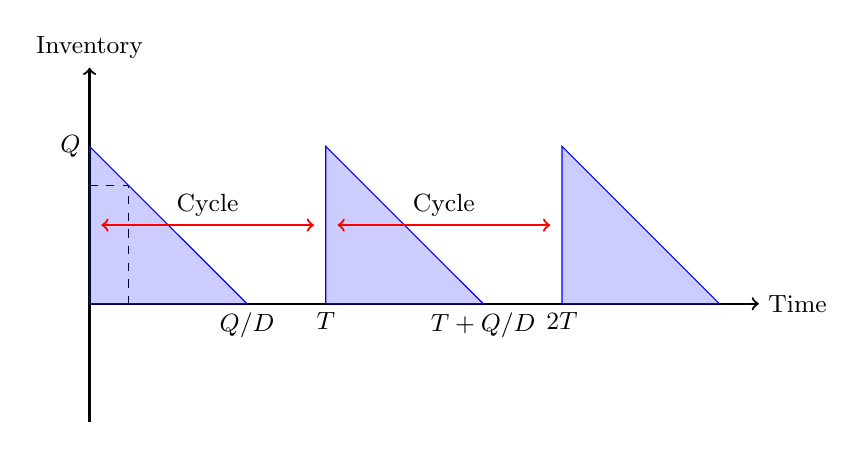
\begin{tikzpicture}[x=1cm,y=0.01cm]
\small

\draw[thick,->] (0,0) -- (8.5,0) node[right] {Time};
\draw[thick,->] (0,-150) -- (0,300) node[above] {Inventory};

\draw[] (0,200) node[left] {$Q$};

%\draw[color=blue,thick] (0,200) -- (3,-100);


%\draw[] (0,150) node[left] {$Q - B - Dt$};
%\draw[] (0.5,0) node[below] {$t$};
\draw[dashed] (0,150) -- (0.5,150) -- (0.5,0);

%\draw[] (2,0) node[below] {$(Q - B) / d$};

\draw[] (2,0) node[below] {$Q/D$};
\draw[] (3,0) node[below] {$T$};

%\draw[color=blue,thick] (3,-100) -- (3,200) -- (6,-100);
%\draw[] (5,0) node[below] {$(2Q - B) / d$};
\draw[] (5,0) node[below] {$T+Q/D$};
\draw[] (6,0) node[below] {$2T$};
%\draw[dashed] (0,200) -- (6,200);
%\draw[dashed] (3,-100) -- (6,-100);

\draw [draw=blue,fill=blue,fill opacity=0.2] (0,0) -- (0,200) -- (2,0) -- cycle;
\draw [draw=blue,fill=blue,fill opacity=0.2] (3,0) -- (3,200) -- (5,0) -- cycle;
\draw [draw=blue,fill=blue,fill opacity=0.2] (6,0) -- (6,200) -- (8,0) -- cycle;

\foreach \y in {0,1}{
	\draw[color=red,thick,<->] (3*\y+0.15,100) -- (3*\y+3-0.15,100);
	\draw[] (3*\y+1.5,100) node[above] {Cycle};}
\end{tikzpicture}
\end{center}

The average cost is the ordering cost plus the inventory cost plus the
cost of lost demand. We already analyzed the cost of the first two
terms. The loss cost is related to all demand lost between the time
$Q/D$ (i.e., the timer it takes the demand to consume $Q$) and the
next order moment $T$. The lost demand is
$DT-Q$. Thus, the average cost becomes
\begin{equation*}
  \begin{split}
  f(Q) 
&= \frac A T + \frac h2 \frac{Q\cdot Q/D}{T}+k \frac{DT-Q}T \\
&= \frac A T + \frac{hQ^2}{2DT}+k (D-\frac QT). 
  \end{split}
\end{equation*}

Take $A=100$, $h=0.2$, $D=20$, $k=1$. As a first attempt, take $T=D/Q^*$ (for the EOQ quantity $Q^*$.) Since $Q^* \approx 141$ and $D=200$, we take $T=200/141\approx 1.4$. \marginpar{This is were I made my first mistake, I copied the wrong numbers.}

\begin{center}
\begin{tikzpicture}[x=0.02cm,y=0.06cm,
declare function = {
f(\Q) = \A/\T+\h/2*\Q/\D*\Q/\T+\k*(\D*\T-\Q); }
]
\small
\def\A{100} 
\def\h{0.2} 
\def\D{20} 
\def\k{1}
%\pgfmathsetmacro{\f}{sqrt(2)*sqrt(\A)*sqrt(\D)*sqrt(\h)}	
\draw[thick,->] (50,-2) -- (470,-2) node[right] {$Q$};
\draw[thick,->] (50,-2) -- (50,75) node[above] {Cost};
\def\T{1.2}
\draw[color=blue,thick,domain=60:400] plot (\x,{f(\x)}) node[right] {$T=\T$};
\def\T{1.5}
\draw[color=red,thick,domain=60:400] plot (\x,{f(\x)}) node[right] {$T=\T$};
\def\T{2.0}
\draw[color=red,thick,domain=60:400] plot (\x,{f(\x)}) node[right] {$T=\T$};
\end{tikzpicture}
\end{center}

Now I wonder why the graph for $T=2$ becomes negative. I guess I did
something wrong, but what?  First I'm checked the cost function. The
only component that can give negative values is
$k(DT-Q)$. \marginpar{As it turned out, I also copied the formula
  incorrectly.} So, when the cost is negative,
I must be considering a combination of $Q$, $D$ and $T$ such that this
term is negative. This only happens when $Q>DT$. But this is strange,
because when $Q>DT$, I am ordering more than the demand that occurs
between two ordering moments, i.e., during the time interval of length
$T$. Clearly then, we must require that $T>Q/D$, which makes
sense. Rechecking also my above estimate for $T$, I notice that I made
stupid algebraic error. It should have been $T=Q^*/D$. For some reason
I also used $D=200$ while it should have been $D=20$. So, let's make a
next attempt with $T=140/20=7$,  use that $Q<DT$, and repair the implementation of the cost function it self (You can't see this in this document, but it is in the source.)

\begin{center}
\begin{tikzpicture}[x=0.02cm,y=0.06cm,
declare function = {
f(\Q) = \A/\T+\h/2*\Q/\D*\Q/\T+\k*(\D-\Q/\T); }
]
\small
\def\A{100} 
\def\h{0.2} 
\def\D{20} 
\def\k{1}
%\pgfmathsetmacro{\f}{sqrt(2)*sqrt(\A)*sqrt(\D)*sqrt(\h)}	
\draw[thick,->] (50,-2) -- (470,-2) node[right] {$Q$};
\draw[thick,->] (50,-2) -- (50,75) node[above] {Cost};
\def\T{7}
\draw[color=blue,thick,domain=60:\D*\T] plot (\x,{f(\x)}) node[right] {$T=\T$};
\def\T{8}
\draw[color=red,thick,domain=60:\D*\T] plot (\x,{f(\x)}) node[right] {$T=\T$};
\def\T{6}
\draw[color=red,thick,domain=60:\D*\T] plot (\x,{f(\x)}) node[right] {$T=\T$};
\end{tikzpicture}
\end{center}

This is too bad: my plotting tool (TikZ) is failing on me, the scales
of the axes are not ok, and I can't read what function belongs to what
graph. In fact, I am now entirely fed up with TikZ, and move to
gnuplot (the tried and tested powertool when it comes to making
plots. With gnuplot I managed to solve the problems in ten minutes. )

\begin{center}
  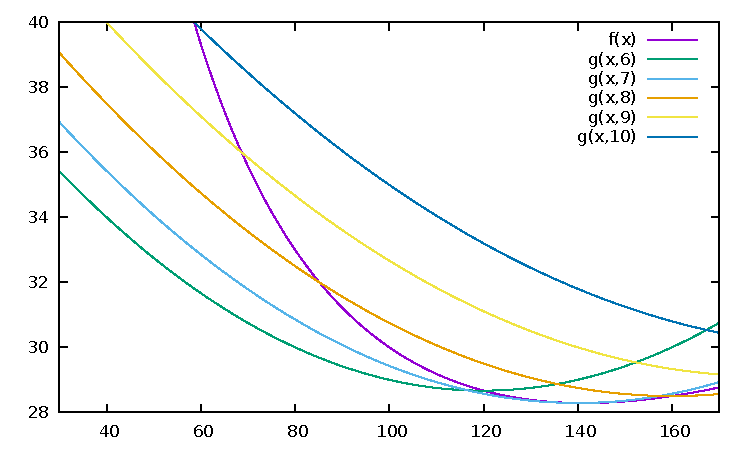
\includegraphics{figures/eoq_loss_0_2}
\end{center}

The situation with $k=0.2$. The $f$ is the graph of the EOQ model, the
$g(x,6)$ is the graph of the cost of the model with loss and with
$T=6$, the $x$ corresponds to the order size $Q$; likewise $g(x,7)$ is
the cost for $T=7$ and so on. We now clearly see that none of the
models with loss achieves a lower cost than the EOQ model with optimal order quantity. 

\begin{center}
  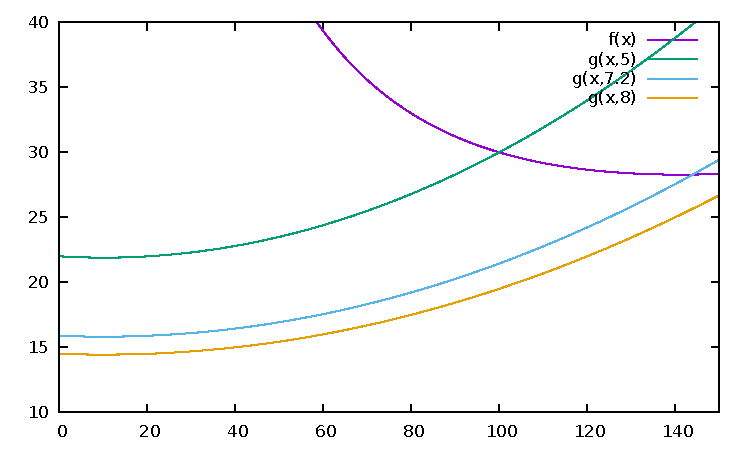
\includegraphics{figures/eoq_loss_0_1}
\end{center}

The situation with $k=0.1$. We now see that when rejecting demand is
pretty cheap, it is best not to order anything: when $Q=0$ the cost is
minimal, hence rejecting all demand seems to be optimal. This is
definitely unexpected!

So, why is that? From the above there seem to be two alternatives,
either order the EOQ and don't reject any demand, or order nothing and
reject all demand.  So, let's trace back the entire analysis.  Indeed,
if we decide to order items and keep them in inventory to satify
demand, then the cost of this must be smaller than the cost of losing
demand. For otherwise, we would simply not be in this business
anyway. So, all in all, this is entirely logical (in hindsight): If
orders are so profitable that you are prepared to keep inventories, it
simply can't be optimal to lose demand. If, however, keeping
inventories is too expensive, it must be optimal not to participate at
all.

Note that this argument is only valid for the case in which everything
is deterministic. In case of stochastic demand, we'll see that
everything changes.

% If we
% reject all demand, then the average cost rate must be $k D$. If, on
% the other hand, we don't want to reject all demand, we order an amount
% $Q$. The cost of ordering is:
% \begin{equation*}
%   \frac A T + \frac{hQ^2}{2DT} - \frac{k Q}{T}.
% \end{equation*}
% Therefore, when this is negative, the overall cost must
% decrease. Thus, if
% \begin{equation*}
%   \frac A T + \frac{hQ^2}{2DT}  < \frac{k Q}{T},
% \end{equation*}
% we must be better off by ordering some amount $Q$. Now it appears that
% all components in this equation are divided by $T$. Removing this
% leads to
% \begin{equation*}
%   A + \frac{hQ^2}{2D}  < k Q.
% \end{equation*}
% But now we see that the cost benefit of ordering $Q$ is independent of
% $T$!



  \end{solution}
\end{question}


\begin{question}
  Continuing on the above question, it might be that items or ordering
  costs are so high that it is better not to `enter the business' at
  all. Can you find a condition to decide whether to keep inventories
  and satisfy demand or reject all demand and have no inventories?
  \begin{solution}
    The cost rate of dropping all demand is $kD$. The cost rate of keeping inventories is, under the EOQ model,  and using that the optimal order quantity $Q^* = \sqrt{2AD/h}$, 
    \begin{equation*}
      \begin{split}
      f(Q^*)
 &= A \frac{D}{Q^*} + \frac h 2 Q \\
 &= A \frac{D}{\sqrt{2AD/h}} + \frac h 2 \sqrt{\frac{2AD}h} \\
 &= A D \sqrt{\frac{h} {2AD}} + \frac h 2 \sqrt{\frac{2AD}h} \\
 &=  \sqrt{\frac {AhD}{2}} + \sqrt\frac{ADh}2 \\
 &=  2\sqrt{\frac {AhD}{2}} \\
 &=  \sqrt{2AhD}.
      \end{split}
    \end{equation*}
When the cost rate of rejecting demand is lower than the cost rate of keeping inventories, we reject the demand, that is, when
\begin{equation*}
kD < \sqrt{2AhD}.
\end{equation*}
We can simplity this a bit to $k^2D^2 < 2AhD$, from which we get
\begin{equation*}
  k^2 D < 2 A h.
\end{equation*}
Thus, when the demand is really small, or the reject cost $k$ is
small, we reject demand. 
  \end{solution}
\end{question}


\begin{question}
  What if we have quantity discounts? What would you do?  
  \begin{solution}
We would need to analyze various alternatives, one alternative for each `ordering regime', since now the ordering cost depends on  the amount we are going to order.

\paragraph{All-unit discounts}

\begin{center}
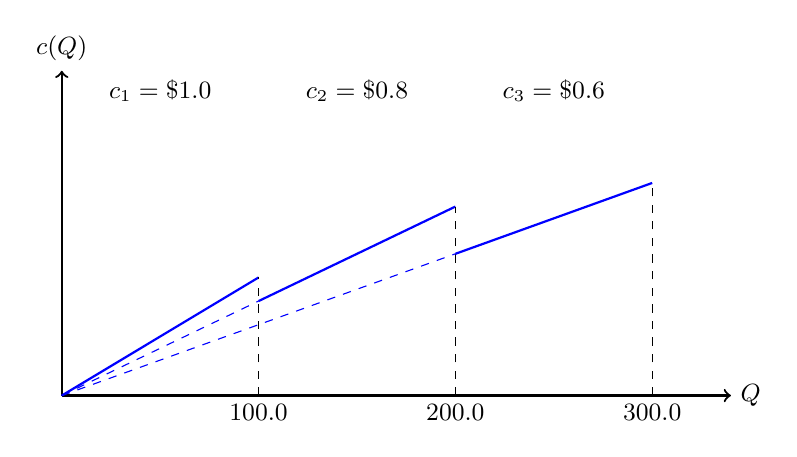
\begin{tikzpicture}[x=0.025cm,y=0.015cm]
\small
\draw[thick,->] (0,0) -- (340,0) node[right] {$Q$};
\draw[thick,->] (0,0) -- (0,275) node[above] {$c(Q)$};
\def\w{100}
\foreach \n/\a in {1/1.0,2/0.8,3/0.6}{
	\pgfmathsetmacro{\s}{(\n-1)*\w}	
	\pgfmathsetmacro{\e}{\n*\w}
	\draw[thick,color=blue,domain=\s:\e] plot (\x,{\a*\x});
	\draw[dashed,color=blue,domain=0:{\s+0.01}] plot (\x,{\a*\x});
	\draw[] (\e,0) -- (\e,0) node[below] {$\e$};
	\draw[dashed] (\e,0) -- (\e,\e*\a);
	\draw[] ({(\s+\e)/2},275) -- ({(\s+\e)/2},275) node[below] {$c_{\n} = \mathdollar\a$};}
\end{tikzpicture}
\end{center}

Average cost per unit time:
\begin{align*}
f(Q) 
& = Kd / Q + cd + hQ/2 \\
& = Kd / Q + cd + \alpha cQ / 2 \quad (h = \alpha c)
\end{align*}

Average cost per unit time:
\begin{equation*}
f(Q) = 
\begin{cases}
Kd / Q + c_1 d + \alpha c_1 Q / 2 & \text{if } 0 \leq Q < Q_1 \\
Kd / Q + c_2 d + \alpha c_2 Q / 2 & \text{if } Q_1 \leq Q < Q_2 \\
Kd / Q + c_3 d + \alpha c_3 Q / 2 & \text{if } Q_2 \leq Q 
\end{cases}
\end{equation*}

\begin{equation*}
f(Q) = 
\begin{cases}
Kd / Q + 1.0 d + \alpha 1.0 Q / 2 & \text{if } 0 \leq Q < 100 \\
Kd / Q + 0.8 d + \alpha 0.8 Q / 2 & \text{if } 100 \leq Q < 200 \\
Kd / Q + 0.6 d + \alpha 0.6 Q / 2 & \text{if } 200 \leq Q 
\end{cases}
\end{equation*}

\begin{equation*}
f(Q) = 
\begin{cases}
2000 / Q + 20 + 0.10 Q & \text{if } 0 \leq Q < 100 \\
2000 / Q + 16 + 0.08 Q & \text{if } 100 \leq Q < 200 \\
2000 / Q + 12 + 0.06 Q & \text{if } 200 \leq Q 
\end{cases}
\end{equation*}

\begin{itemize}
\item $c_1 = \mathdollar 1.0$, $c_2 = \mathdollar 0.8$, $c_3 = \mathdollar 0.6$
\item $Q_1 = 100$, $Q_2 = 200$
\end{itemize}

\begin{itemize}
\item $K = \mathdollar 100$
\item $\alpha = 0.2$, $d = 20$ units
\end{itemize}

\begin{center}
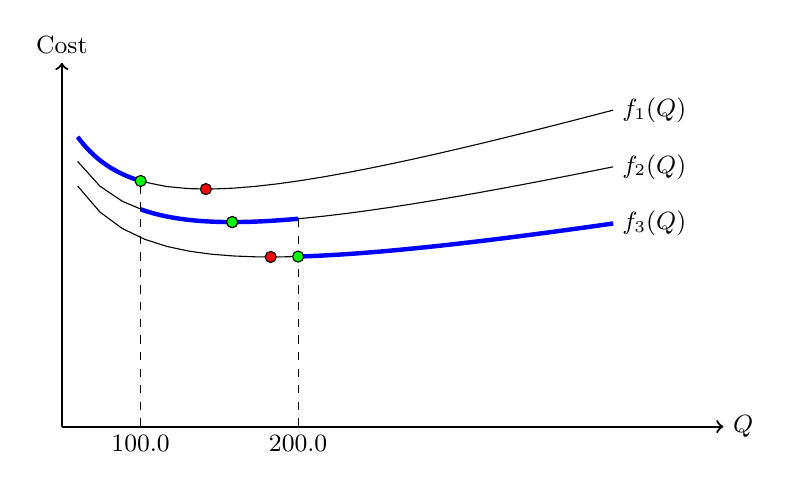
\begin{tikzpicture}[x=0.02cm,y=0.06cm]
\small
\def\c{1} 
\def\K{100} 
\def\h{0.2} 
\def\d{20} 
\def\alpha{0.2}
\def\w{100}
\draw[thick,->] (50,-2) -- (470,-2) node[right] {$Q$};
\draw[thick,->] (50,-2) -- (50,75) node[above] {Cost};
\foreach \n/\c in {1/1.0,2/0.8,3/0.6} {
	\pgfmathsetmacro{\h}{\alpha*\c}	
	\pgfmathsetmacro{\Q}{sqrt(2)*sqrt(\K)*sqrt(\d)/sqrt(\h)}
	\pgfmathsetmacro{\f}{sqrt(2)*sqrt(\K)*sqrt(\d)*sqrt(\h)+\c*\d}	
	\pgfmathsetmacro{\s}{(\n-1)*\w}	
	\pgfmathsetmacro{\e}{\n*\w}

	\draw[domain=60:400] plot (\x,{\d*\K/\x+\c*\d+\h*\x/2}) node[right] {$f_{\n}(Q)$};

	\ifnum\n<3
		\draw[color=blue,ultra thick,domain={max(60,\s}:\e] plot (\x,{\d*\K/\x+\c*\d+\h*\x/2});
		\draw[dashed] (\e,-2) -- (\e,{\d*\K/\e+\c*\d+\h*\e/2});
		\draw (\e,-2) node[below] {$\e$};
	\else
		\draw[color=blue,ultra thick,domain={max(60,\s}:400] plot (\x,{\d*\K/\x+\c*\d+\h*\x/2});
	\fi

	\draw [fill=red] (\Q,\f) circle (2pt);

	\pgfmathparse{int(\Q-\s)}
	\ifnum \pgfmathresult < 0
		\draw [fill=green] (\s,{\d*\K/\s+\c*\d+\h*\s/2}) circle (2pt);
	\fi
	\pgfmathparse{int(\Q-\e)}
	\ifnum \pgfmathresult > 0
		\draw [fill=green] (\e,{\d*\K/\e+\c*\d+\h*\e/2}) circle (2pt);
	\fi
	\pgfmathparse{int((\Q-\e)*(\Q-\s))}
	\ifnum \pgfmathresult < 0
		\draw [fill=green] (\Q,\f) circle (2pt);
	\fi
}
\end{tikzpicture}
\end{center}

Optimization:
\begin{itemize}
\item global optimum $\rightarrow$ check breakpoints and local minimums and compare average total costs
\end{itemize}


\paragraph{incremental discounts}

\begin{center}
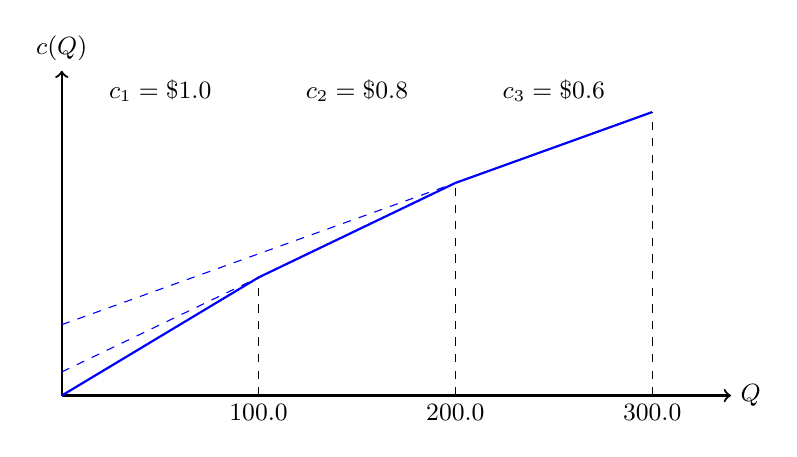
\begin{tikzpicture}[x=0.025cm,y=0.015cm]
\small
\draw[thick,->] (0,0) -- (340,0) node[right] {$Q$};
\draw[thick,->] (0,0) -- (0,275) node[above] {$c(Q)$};
\def\w{100}
\pgfmathsetmacro{\b}{0}
\foreach \n/\a/\b in {1/1.0/0,2/0.8/20,3/0.6/60}{
	\pgfmathsetmacro{\s}{(\n-1)*\w}	
	\pgfmathsetmacro{\e}{\n*\w}
	\draw[thick,color=blue,domain=\s:\e] plot (\x,{\a*\x+\b});
	\draw[dashed,color=blue,domain=0:{\s+0.01}] plot (\x,{\a*\x+\b});
	\draw[] (\e,0) -- (\e,0) node[below] {$\e$};
	\draw[dashed] (\e,0) -- (\e,\e*\a+\b);
	\draw[] ({(\s+\e)/2},275) -- ({(\s+\e)/2},275) node[below] {$c_{\n} = \mathdollar\a$};}
\end{tikzpicture}
\end{center}

Average cost per unit time:
\begin{align*}
f(Q) 
& = Kd / Q + cd + hQ / 2 \\
& = Kd / Q + c(Q)d/Q + \alpha c(Q)/2 \quad (c = c(Q)/Q, h = \alpha c)
\end{align*}

Average variable cost:

\begin{equation*}
c(Q) = 
\begin{cases}
c_1 Q & \text{if } 0 \leq Q < Q_1 \\
c_1 Q_1 + c_2(Q - Q_1) & \text{if } Q_1 \leq Q < Q_2 \\
c_1 Q_1 + c_2(Q_2 - Q_1) + c_3(Q - Q_2) & \text{if } Q_2 \leq Q 
\end{cases}
\end{equation*}


\begin{equation*}
c(Q) = 
\begin{cases}
Q & \text{if } 0 \leq Q < 100 \\
20 + 0.8Q & \text{if } 100 \leq Q < 200 \\
60 + 0.6Q & \text{if } 200 \leq Q 
\end{cases}
\end{equation*}

Average cost per unit time:

\begin{equation*}
f(Q) = Kd / Q + c(Q)d / Q + \alpha c(Q) / 2
\end{equation*}

\begin{equation*}
f(Q) = 2000 / Q + c(Q)20 / Q + 0.1 c(Q)
\end{equation*}

\begin{itemize}
\item $c_1 = \mathdollar 1.0$, $c_2 = \mathdollar 0.8$, $c_3 = \mathdollar 0.6$
\item $Q_1 = 100$, $Q_2 = 200$
\end{itemize}

\begin{itemize}
\item $K = \mathdollar 100$
\item $\alpha = 0.2$, $d = 20$ units
\end{itemize}

Average cost per unit time: (convex for each segment)
\begin{equation*}
f(Q) = 
\begin{cases}
2000 / Q + 20 + 0.10Q & \text{if } 0 \leq Q < Q_1 \\
2400 / Q + 18 + 0.08Q & \text{if } Q_1 \leq Q < Q_2 \\
3200 / Q + 18 + 0.06Q & \text{if } Q_2 \leq Q 
\end{cases}
\end{equation*}

\begin{center}
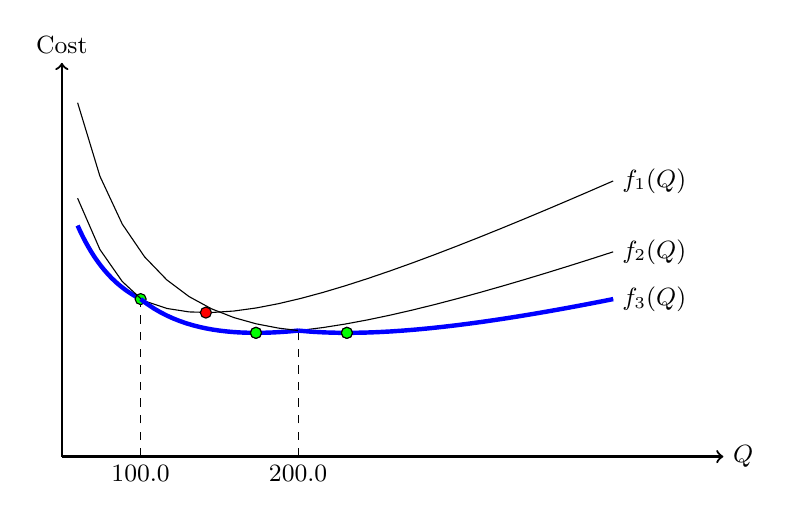
\begin{tikzpicture}[x=0.02cm,y=0.10cm]
\small
\def\c{1} 
\def\K{100} 
\def\h{0.2} 
\def\d{20} 
\def\alpha{0.2}
\def\w{100}
\draw[thick,->] (50,30) -- (470,30) node[right] {$Q$};
\draw[thick,->] (50,30) -- (50,80) node[above] {Cost};
\foreach \n/\a/\b/\c in {1/2000/20/0.1,2/2400/18/0.08,3/3200/18/0.06} {
	\pgfmathsetmacro{\Q}{sqrt(\a)/sqrt(\c)}	
	\pgfmathsetmacro{\f}{\a/\Q+\b+\c*\Q}	
	\pgfmathsetmacro{\s}{(\n-1)*\w}	
	\pgfmathsetmacro{\e}{\n*\w}

	\draw[domain=60:400] plot (\x,{\a/\x+\b+\c*\x}) node[right] {$f_{\n}(Q)$};

	\ifnum\n<3
		\draw[color=blue,ultra thick,domain={max(60,\s}:\e] plot (\x,{\a/\x+\b+\c*\x});
		\draw[dashed] (\e,30) -- (\e,{\a/\e+\b+\c*\e});
		\draw (\e,30) node[below] {$\e$};
	\else
		\draw[color=blue,ultra thick,domain={max(60,\s}:400] plot (\x,{\a/\x+\b+\c*\x});
	\fi

	\draw [fill=red] (\Q,\f) circle (2pt);

	\pgfmathparse{int(\Q-\s)}
	\ifnum \pgfmathresult < 0
		\draw [fill=green] (\s,{\a/\s+\b+\c*\s}) circle (2pt);
	\fi
	\pgfmathparse{int(\Q-\e)}
	\ifnum \pgfmathresult > 0
		\draw [fill=green] (\e,{\a/\e+\b+\c*\e}) circle (2pt);
	\fi
	\pgfmathparse{int((\Q-\e)*(\Q-\s))}
	\ifnum \pgfmathresult < 0
		\draw [fill=green] (\Q,\f) circle (2pt);
	\fi
}
\end{tikzpicture}
\end{center}

Optimization:
\begin{itemize}
\item global optimum $\rightarrow$ check breakpoints and local minimums and compare average total costs
\end{itemize}
  \end{solution}
\end{question}



\begin{question}
EOQ with joint ordering
  \begin{solution}
    TBD
  \end{solution}
\end{question}

\begin{question}
  Consider the setting of the EOQ model but now with batchsize
  constraints, that is, the order quantity is in multiples of some number $q$, say. Can you make a formula for the cost, and find the minimum?
  \begin{solution}
This is, in fact, really easy. Suppose we order $n$ times the minimal order quantity $q$. Then, for a yearly demand $D$, ordering cost $A$, and inventory cost $h$, we pay per year
\begin{equation*}
  A \frac{D}{nq} + h\frac{nq}2 = A\frac{D/q}n + hq\frac{n}2.
\end{equation*}
But this is precisely the normal EOQ model with demand $D'=D/q$ and inventory cost $h'=hq$. Thus, the optimal number of batches to order is:
\begin{equation*}
  n^2 = \frac{2D'A}{h'} = \frac{2AD/q}{hq} = \frac{2AD}{hq^2}.
\end{equation*}
Hence, the optimal $n$ expressed in the EOQ quantity $Q^*$ is 
\begin{equation*}
  n = \sqrt{\frac{2AD}{h}}\frac1q=\frac{Q^*}q.
\end{equation*}
  \end{solution}
\end{question}


\begin{question}
EOQ with yield loss
  \begin{solution}
    TBD
  \end{solution}
\end{question}

\begin{question}
EOQ with lower salvage value
  \begin{solution}
    TBD
  \end{solution}
\end{question}


\begin{question}
EOQ with constraints on cycle length

EOQ under periodic review rather than continuous review.

Constraints on when to order, order moment.

  \begin{solution}
    TBD
  \end{solution}
\end{question}


\begin{question}
  EOQ with positive replenishment lead time and variance in the lead
  time.

  \begin{solution}
    TBD

Suddenly we have to deal with safety stock!
  \end{solution}
\end{question}

\begin{question}
  Suppose that the delivery rate of the items we order is not
  `infinite', as it is in the EOQ setting (recall, in the EOQ we
  assume instantaneous deliveries). If we have a machine that
  replenishes the FGI we have to take into account the production
  rate, $r$ say. If it costs $K$ to switch on the machine, when do you switch the machine on or off?
  \begin{solution}
    An easy policy is to switch the machine on when the FGI level hits
    some level $Q$, and switch it off when the level is $0$. Of course
    we need to assume that $D<r$, i.e., the production rate is larger
    than the demand rate $D$. 

    To find an expression to cover this situation we can reason like
    this.  When the machine is on, inventory increases at rate
    $r-D$. If we keep it on for $T$ time units, then the inventory
    level is $T(r-D)$ when we switch off. The time until the inventory
    hits 0 is then $T(r-D)/D$, since we start with an inventory level
    $T(r-D)$ after switching off and the demand rate is $D$. Thus, the total cycle length is
    \begin{equation*}
      T + \frac{T(r-D)}D = T + T(\frac{r}D-1) = T + T\frac r D - T = T\frac r D.
    \end{equation*}

    What is, in the EOQ, the average inventory cost? It is half the
    maximal height times $h$, i.e., $hQ/2$. In our present case, the
    maximal height is $T(r-D)$. Thus the average inventory cost must
    be  $hT(r-D)/2$. 

    The ordering cost in the EOQ is $A$ times the order frequency, i.e., $A D/Q$. Here the time between two `order' moments (switching moments) is $Tr/D$. Hence, the frequency is $D/rT$ and the average switching cost is $K D/rT$. 

All in all we get for the average cost
\begin{equation*}
  \frac{h(r-D)}2 T + \frac{K}r \frac DT.
\end{equation*}
This is similar to the EOQ model with $h'=h(r-D)$ and $A=K/r$. But then the optimal $T$ must be given by
\begin{equation*}
  T = \sqrt{\frac{2AD}{h'}} = \sqrt{\frac{2DK/r}{h(r-D)}}=\sqrt{\frac{2DK}{hr(r-D)}}.
\end{equation*}
  \end{solution}
\end{question}


\begin{question}
EOQ with variable demand.
  \begin{solution}
    TBD
  \end{solution}
\end{question}

\begin{question}
Wagner Whitin
  \begin{solution}
    TBD
  \end{solution}
\end{question}

\begin{question}
Silver meal
  \begin{solution}
    TBD
  \end{solution}
\end{question}

\begin{question}
Where to put the I/O interface? For what product/item?
  \begin{solution}
    TBD
  \end{solution}
\end{question}

\begin{question}
  What is the difference between continuous and period review? Why/when to prefer one over the other?
  \begin{solution}
    TBD
  \end{solution}
\end{question}

\begin{question}
  What is the difference between fixed order and order-up-to policies?
  Why/when to prefer one over the other?
  \begin{solution}
    TBD

Order quantities

  \end{solution}
\end{question}

\begin{question}
  What  different type of service level can you define?
  Why/when to prefer one over the other?
  \begin{solution}
    TBD

e.g. cycle service level.
  \end{solution}
\end{question}

\begin{question}
  Why to use safefy stock? What is it? 
  \begin{solution}
    TBD
  \end{solution}
\end{question}

\begin{question}
  Are lead times typically (approximately) constant ore variable?
  \begin{solution}
    TBD
  \end{solution}
\end{question}



\subsection{Strategic impact of short leadtimes/small inventories,
  what if lead time is a control?}

You run a pharmaceutical company. The medicines you sell need to be
packaged. The price quotation of the company that prints the packages
depends on the order size $Q$.
  \begin{itemize}
  \item If $Q$ covers 2 weeks of demand: price per unit is 1.15 Euro
  \item If $Q$ covers 1 month of demand: price per unit is 1. Euro
  \item If $Q$ covers 2 months of demand: price per unit is 0.95 Euro
  \item If $Q$ covers 3 months of demand: price per unit is 0.9 Euro
  \item If $Q$ covers 6 months of demand: price per unit is 0.85 Euro
  \end{itemize}
The problem is to determine how much to order.

\begin{question}
  \begin{itemize}
  \item Include your own storage cost, i.e., packages need to be
    stored as your raw materials inventory.  Suppose the
    inventory cost is $20\%$ per unit per year. Can we now compute the
    inventory cost?  Assume that $D = 12000$ units per year.
  \item Include transportation cost.  Assume that $A = 50$ Euro.
  \end{itemize}
\end{question}

\begin{question}
Every so often government regulations change. As a result, the entire
stock becomes obsolete. What now?
\begin{solution}
  \begin{itemize}
  \item Use data to make assumptions on the probability that the
    remaining stock will be affected by a regulation change.
  \item Assume that a regulation change occurs, on average, every
    month, and time to implement the change is one month.
  \item If  $Q$ is 2 weeks of demand, then?  there is no problem
  \item If $Q$ is 3 months of demand, then? 
  \end{itemize}
Challenge: Can you compute the optimal order quantity in this situation? 

%   \begin{lstlisting}%{python}
% A = 50.
% D = 12000
% h = 0.2

% def C(Q, p): # return average yearly inventory cost
%     # p is price per unit, so that
%     # p*h is the inventory cost per unit per year
%     cost = A*D/Q + h*p*Q/2.
%     return cost

% def output(Q, p, period):
%     print("Yearly inventory costs %s: %3.2f; price of a batch: %3.2f"%(period, C(Q, p), Q*p))

% output(D/24, 1.15, "2 weeks")
% #Likewise for the other cases.
%   \end{lstlisting}

%   \begin{minted}{python}
% Yearly costs 2 weeks: 1257.50; batch price: 575.00
% Yearly costs 1 month: 700.00; batch price: 1000.00
% Yearly costs 2 months: 490.00; batch price: 1900.00
% Yearly costs 3 months: 470.00; batch price: 2700.00
% Yearly costs 6 months: 610.00; batch price: 5100.00
%   \end{minted}

What are the consequences?

  \begin{itemize}
    \item For some customers short lead times are very important. So important
      they are willing to pay significantly more per unit.
    \item For some customers small batch sizes are very important. So
      important they are willing to pay significantly more per unit.
    \item Thus,  it is essential for some/many companies to be
      able to offer short and predictable lead times and produce in
      small batches.
    \item Producing in small batches can be achieved with slack capacity and short setup times and low setup costs.
    \item Short and predictable lead times can be achieved with conwip
      and a order prioritization (priority queues)
  \end{itemize}
\end{solution}
\end{question}

% \subsection{News boy/vendor model}

We use the notation of Factory Physics (FP). Note that the formulas in
FP are in terms of integrals rather than with summations. We find this
unsatisfactory since it is easy to evaluate summations in excel (or an
other programming environment), and carrying out integration is often
much more difficult. For this reason we derive  results of FP in terms
of summations. 


We develop the newsvendor in stages.  Suppose that a shop sells some
perishable item with a life time of one day. It has to decide one day
ahead, or the morning before the shop opens, on the number of items to
order/make/prepare. The costs are
\begin{align*}
  p_b &= 5, \text{i.e., Buying price of one item} \\
  p_s &= 10,  \text{i.e., Selling  price of one item} \\
  p_e &= 3, \text{i.e, Salvage (end) value of one item} \\
  c_o &= \text{i.e., Overage cost, Cost of having  one  item over at the end of the day} \\
  c_s &= \text{i.e., Shortage cost, Cost of being   one  item short during the day} \\
\end{align*}
Cost for overage or underage are linear.  Let $X$ (a random variable)
be the number of units sold during a particular period, and let $Q$
denote the number of units ordered.  I assume that
$g_i = \P\{ X = i\}$ is given.


\begin{exercise}
  Can you express $c_o$ and $c_s$ in terms of the other cost parameters?
  \begin{comment}
    $c_o = p_b-p_e$ and $c_s = p_s-p_b$. 
  \end{comment}
\end{exercise}


\begin{exercise}
Suppose the daily demand is $X\in \{0,1\}$ and $g(0) = \P(X=0)=1/2 = g(1)$. What would be the best number of items $Q$ to make? 
\begin{comment}
  The profit of the choice $Q=0$ is 0. Now consider $Q=1$. What is the profit?  We pay for one unit, and sell it perhaps. If we don't sell it, we get the salvage value, if we sell it, we get the sales price. Thus, the profit is
  \begin{equation*}
    -p_b 1 + p_s\cdot 1/2 + p_e\cdot 1/2. 
  \end{equation*}
\end{comment}
\end{exercise}

\begin{exercise}
Suppose the daily demand is $X\in \{0,1\}$ and $g(0) = \P(X=0)=1/3 = 1- g(1)$. What would be the best number of items $Q$ to make? 
\begin{comment}
If $Q=1$ we make as a profit:
  \begin{equation*}
    -p_b 1 + p_s\cdot 2/3 + p_e\cdot 1/3 = -5 + 20/3 + 1> 0
  \end{equation*}
So, ordering $Q$ leads to a higher profit than ordering $Q=0$.
\end{comment}
\end{exercise}


\begin{exercise}
  What are the general terms that make up the profit function $Z(Q)$ if you were to order $Q$? 
  \begin{comment}
If you would order an amount $Q$, the profit consist of three terms: 
  \begin{itemize}
  \item expected number sold
  \item expected number left over
  \item order size
  \end{itemize}
  For the expected number of items sold, if the demand $X$ on a day
  turns out to be smaller than $Q$, we sell $X$; if $X>Q$ we only sell
  $Q$. Therefore, the expected sales is
  \begin{equation*}
    \E(\min\{Q,X\}). 
  \end{equation*}
The expected number of items over is $Q$ minus the expected sales: 
  \begin{equation*}
    Q-\E(\min\{Q,X\}) = 
    \E(Q-\min\{Q,X\})
  \end{equation*}
  where the second equation follows from the observation that the
  expected value of a constant is the constant itself, i.e.,
  $Q=\E(Q)$.  Thus, the total profit of buying $Q$ items must be
\begin{equation*}
Z(Q)=  -p_bQ+p_s\E(\min\{Q,X\}) + p_e\E(Q-\min\{Q,X\}).
\end{equation*}
  \end{comment}
\end{exercise}

\begin{exercise}
  Write $\E(X)$, i.e., the expected demand in terms of a summation.
  \begin{comment}
Recall that $\E(X)$ is just a short-hand for
    \begin{equation*}
      \E(X) = \sum_{i=0}^\infty i g(i).
    \end{equation*}
  \end{comment}
\end{exercise}

\begin{exercise}
  Can you write $\E(\min\{X,Q\}$ in terms of probabilities $g(i) = \P(X=i)$?
  \begin{comment}
From the previous exercise,
\begin{equation*}
  \E(\min\{(X,Q\})) = \sum_{i=0}^\infty \min(i,Q)g(i) = \sum_{i=0}^Q i g(i) + \sum_{i=Q+1}^\infty Q g(i).
\end{equation*}
Observe that $\sum_{i=Q+1}^\infty g(i)=\P(X\geq Q+1)$, thus we can simplify the above to
\begin{equation*}
  \E(\min\{(X,Q\})) = \sum_{i=0}^Q i g(i) + Q\P(X\geq Q+1).
\end{equation*}
  \end{comment}
\end{exercise}

\begin{exercise}
  Suppose for our example that the daily demand is $X\in \{0,1,2\}$
  and $g(0) = \P(X=0)=1/4$, $g(1)=1/3$, $g(2)=5/12$. What would be the
  best number of items $Q$ to make?
\begin{comment}
  Now we need to consider three different $Q$'s, $Q=0, 1,$ or $2$.
  Suppose that $Q=1$, then
\begin{equation*}
    \E(\min\{Q,X\}). =   \E(\min\{1,X\}). =   0\P(X=0) + 1\P(X=1)+1\P(X=2) = 1\cdot 1/3+1\cdot 5/12=9/12=3/4.
\end{equation*}
The expected number of items over is $Q$ minus the expected sales: 
  \begin{equation*}
    \E(Q-\min\{Q,X\}) = 1-3/4=1/4
  \end{equation*}
Thus,  for the example, the total profit is
\begin{equation*}
  -5\cdot1 + 10\cdot3/4+3\cdot1/4
\end{equation*}
is the expected profit per day of buying $Q=1$ at the start of the day. 

Once you implement this in excel, it is easy to experiment with
different values of $Q$ and see what is the best choice for $Q$. 
\end{comment}
\end{exercise}


\begin{exercise}
If the demand can be quite big, e.g., $X\in\{0,1,\ldots, 1000\}$, what is the slope of $Z(Q)$ for $Q$ small? What is the slope if $Q$ is big, i.e., near 1000? Assume that the demand distribution is something reasonable.
\begin{comment}
  If $Q=1$ it is very unlikely that the item will not be sold. In fact, we are nearly sure it will be sold, hence, the slope of $Z$ for small $Q$ must be $p_s$. If $Q$ is very large, we are pretty sure the `last item' will not be sold, hence, the slope must be $-p_e$. 
\end{comment}
\end{exercise}

\begin{exercise}
  Suppose there would be a setup cost which you have to pay to order any positive amount $Q>1$. What is then the profit? 
  \begin{comment}
    This is a no-brainer. If the setup cost is $s$, then just subtract
    $s$ from the profit function $Z(Q)$.
  \end{comment}
\end{exercise}

\begin{exercise}
Suppose we would set a certain service level, what is the profit under such a service level? Before we tackle this, what type of service level can we consider? 
\begin{comment}
  Cycle service level $P_1$, i.e., the probability that there are more
  items than demand, i.e., the fraction of periods/days that the shop
  does not run out of stock:
\begin{equation*}
P(X\leq Q) \geq P_1.
\end{equation*}

Another interesting service level is the fraction of demand that is met, i.e., the fill rate must be higher than some level $P_2$:
\begin{equation*}
\E(\min\{Q, X\})/ \E(X) \geq P_2
\end{equation*}
Realize that $\E(\min\{Q, X\})$ is the expected sales, while $\E(X)$ is the expected demand. The average amount of demand met is the sales divided by the demand.
\end{comment}
\end{exercise}

\begin{exercise}
  Now we can consider the profit under setting a certain performance level. How would you compute this?
  \begin{comment}
    If we want to focus on fill rate, first determine $Q$ such that
    $\E(\min\{Q, X\})/ \E(X) \geq P_2$, where $P_2=90\%$ or so. Call
    this $Q_2$. Then compute $Z(Q_2)$ to get the profit. 

    If we want to focus on cycle service level rate, first determine
    $Q$ such that $\P(X\leq Q) \geq P_1$, where $P_1=80\%$ or so. Call
    this quantity $Q_1$. Compute now $Z(Q_1$ to get the profit.
  \end{comment}
\end{exercise}

We next  discuss a few expressions that simplify the implementation of the profit function in excel.

\begin{exercise}
  Explain that $\E( \max\{Q-X, 0\})$ is another expression for the expected number of items over.
  \begin{comment}
    If $Q>X$, we have $Q-X$ over, if $Q\leq X$ we don't have items over. 
  \end{comment}
\end{exercise}

\begin{exercise}
  Write $\E (\max\{Q-X, 0\}) $ as a summation, so that you can implement this in excel.
  \begin{comment}
\begin{equation*}
  \begin{split}
  \E( \max\{Q-X, 0\} )
  &= \sum_{i=0}^\infty \max\{Q-i,0\}\P\{X=i\}\\
  &= \sum_{i=0}^\infty \max\{Q-i,0\}g_i\\
  &= \sum_{i=0}^Q (Q-i) g_i \\
  &= (Q-0) g_0 + (Q-1)g_1+ \cdots (Q-(Q-1))g_{Q-1} + (Q-Q)g_Q\\
  &= (Q-0) g_0 + (Q-1)g_1+ \cdots (Q-(Q-1))g_{Q-1} + 0 g_Q\\
  &= \sum_{i=0}^{Q-1} (Q-i) g_i.
  \end{split}
\end{equation*}
  \end{comment}
\end{exercise}


\begin{exercise}
  Why is $ \E( \max\{X-Q, 0\})$ the expected number of items short?
  \begin{comment}
    If there is a shortage of items, it must be that $X>Q$. The amount short is $X-Q$.
  \end{comment}
\end{exercise}

\begin{exercise}
  Write $\E (\max\{X-Q, 0\}) $ as a summation.
  \begin{comment}
\begin{equation*}
\begin{split}
     \E (\max\{X-Q, 0\} )
   &= \sum_{i=0}^\infty \max\{i-Q,0\}g_i\\
   &= \sum_{i=Q}^\infty (i-Q) g_i \\
   &= \sum_{i=Q+1}^\infty (i-Q) g_i.
\end{split}
\end{equation*}
\end{comment}
\end{exercise}


\begin{exercise}
  Let $Q=3$ and $g_1=g_2\ldots=g_5 = 1/5$. Compute $\theta = \E(X)$, i.e., the expected demand, the expected lost sales and the expected number over.
  \begin{comment}
    \begin{align*}
      \E( X) &= \sum_{i=1}^5 i g_i = 1/5+2/5+\cdots+5/5 = 3, \\
      \E (\max\{X-Q,0\}) &= \sum_{i=Q+1}^5 (i-Q) g_i = (4-3)/5 + (5-3)/5,\\
      \E (\max\{Q-X,0\}) &= \sum_{i=1}^{Q-1} (Q-i) g_i = (3-1)/5 + (3-2)/5.
    \end{align*}
  \end{comment}
\end{exercise}

\begin{exercise}
  Up to now we considered the profit function $Z(Q)$.  Can you
  establish a cost function of the newsvendor problem?
  \begin{comment}
The expected cost resulting from ordering an amount $Q$ follows
from combining the above formulas:
\begin{equation*}
     Y(Q) = c_o  \E( \max\{Q-X, 0\})  +   c_s \E( \max\{X-Q, 0\}) - c_s\E(X).
\end{equation*}
Note that the expected `cost' of selling $\E(X)$ of items should be subtracted from the cost. Since this term does not depend on the decision variable $Q$, it is often left out of the cost function, but formally it should be there.
  \end{comment}
\end{exercise}


\begin{exercise}
  Show that the profit is minus the the cost, i.e., $Z(Q) = -Y(Q)$.
  \begin{comment}
    Here we go:
    \begin{equation*}
      \begin{split}
        Z(Q) 
&=  -p_bQ+p_s\E(\min\{Q,X\}) + p_e\E(Q-\min\{Q,X\}) \\
&=  (p_e - p_b)Q+ p_s(\E(\min\{Q,X\}) - p_e\E(\min\{Q,X\}) \\
&=  (p_e - p_b)Q+ (p_s-p_e)(\E(\min\{Q,X\})\\
&=  -c_oQ+ (c_o+c_s)(\E(\min\{Q,X\})\\
&=  -c_o( Q - \E(\min\{Q,X\})) - c_s(\E(X) - \E(\min\{Q,X\}) + c_s\E(X)\\
&=  -c_o \E(Q-\min\{Q,X\}) - c_s\E(X-\min\{Q,X\}) + c_s\E(X)\\
&=  -c_o \E(\max\{Q-X,0\}) - c_s\E(\max\{X-Q,0\}) + c_s\E(X)\\
&=  -Y(Q).
      \end{split}
    \end{equation*}
Ensure you understand the last two steps. 
  \end{comment}
\end{exercise}

\begin{exercise}
Reproduce the results of the Christmas Lights Example of Factory Physics.
\begin{comment}
  First the data. We also use a library to handle the computations for
  the normal distribution. 


\begin{minted}[mathescape, fontsize=\small, xleftmargin=0.5em]{python}
from scipy.stats import norm
c_o = 5 - 2.5
c_s = 10 - 5
mu = 10000
sigma = 1000
X = norm(loc=mu, scale=sigma) # demand
\end{minted}


The result of the book is easy to produce. 


\begin{minted}[fontsize=\footnotesize, xleftmargin=0.5em, mathescape]{python}
>>> critical_fractile = c_s / (c_o + c_s)
>>>
>>> Q_star = X.ppf(critical_fractile)
>>> Q_star
10430.727299295457

\end{minted}

\end{comment}
\end{exercise}

\begin{exercise}
  In this christmas light example, 
do you think that $\sigma = 1000$ is reasonable? 
  \begin{comment}
    In all honesty, I think it is way too small. I would say that
    $\sigma=5000$ is much more reasonable. The problem is that if you
    would use this larger value, i.e., $\sigma=5000$, in the normal
    distribution, the probability that the demand is
    $\P(X<0)=\Phi((X-\mu)/\sigma < 0$ is not small anymore. However,
    the demand cannot be negative, hence using the normal distribution
    as an approximation of the demand is wrong for such cases. 

    Now this happens quite often: The problems in the books are tuned
    to showcase the simple methods developed in the book. However, as
    soon you have to do something real, the simple tricks all of a
    sudden don't work anymore. 
  \end{comment}
\end{exercise}


\begin{exercise} A Case to  Get rich in one day. 

  \begin{itemize}
  \item You plan to sell Napoleons tomorrow just outside of the
    Duisenberg building.
  \item How much money can you make? 
  \item How many Napoleons would you order today, to sell tomorrow?
  \end{itemize}
  Realize that this case contains a number of the problems related to
  dealing with perishable inventory, e.g., fashion. 

   
\includegraphics[scale = 1.0]{figures/mille-feuille}

   \begin{comment}
Here are the steps.
  \begin{itemize}
  \item Let's first assume that demand is normally distributed. Then
    we know from FP that $Q$ should be such that
    $G(Q) = c_s/(c_s+c_o)$.
  \item We make some assumptions about the prices. Take $p_s=0.75$,
    $p_b = 0.25$. $p_e=0$. Hence, $c_o = 0.25$, and $c_s = 0.5$.
  \item Thus, the critical fraction is $c_s/(c_s+c_o)=0.5/0.75 = 2/3$.
  \item Now compute $z$ with $\Phi(z)=2/3.$. Hence $z=0.43$.
  \item We also need some idea about the demand. How to get this?
  \item For Napoleons, we don't have yesterday's demand \ldots
  \item Can we use demand data of similar products?  I don't know what
    data to use. I have never tried to sell napoleons.
  \item Can we ask our sales force?  no. We don't have a sales force. 
  \item Last resort: make an educated guess; use powers of ten
    trick. Under this price model, I expect to sell more 1 napoleon,
    also more than 10, 100 might be, 1000 is too much. So, take
    $\mu=100$ as an estimate. Since I am not sure, $\sigma=30$ seems
    reasonable.
  \item If $\mu = 100$ and $\sigma = 30$, then $Q=0.43\sigma + \mu \approx 112$.
  \item Finally, what is the profit $Z(Q)$?
\item With the above formulas you can compute $Z(Q)$,  but let's use handwaving for a quick estimate. 
\item Note that $\min\{Q, X\} \leq X$, hence
  $\E \min\{X, Q\} \leq \E X= \mu$. If $\E \min\{X, Q\}\approx 95$,
  then $Z(112) \approx 95p_s - 100 p_b = 95\cdot 0.75 - 100 \cdot 0.25$.
  Since $95\approx100$, use this to simplify yet more:
  $Z(112) \approx 100(0.75-0.25) = 50$ Euro.
\item There are easier ways to make money!
  \end{itemize}
\end{comment}
\end{exercise}

\begin{exercise}
   Summarize the approach we took to some insight into this napoleon
   case, even though, initially, we had no idea about what profit we
   could make.
   \begin{comment}
Conclusion.
  \begin{itemize}
  \item Determine/estimate relation between demand (distribution) and sales price
  \item Make plots of the profit $Z$ as a function of $Q$, the demand
    distribution, and the sales price.
  \item Choose a $Q$ that makes sense. The existence of an optimal $Q$
    is a \emph{delusion}.
  \item Be aware that salesforce may predict too high demand. They get insentives to sell much, but they are not responsible for overage cost!
  \end{itemize}
   \end{comment}
 \end{exercise}


%%% Local Variables:
%%% mode: latex
%%% TeX-master: "notes_all"
%%% End:

% \subsection{Two-Stage Newsvendor Model}

Let us consider a case where we have a two-period planning horizon, rather than one as we had for the newsvendor problem. Here, at the beginning of each period, we  first observe the current inventory level, and then we decide upon the order quantity. Thus, this case  becomes an extension of the newsvendor model, because now we have an extra ordering moment in the middle of the day. 

For convenience, we use the same notation that we used for the single-period newsvendor model. However, we add a period index to the buying and selling prices as well as the demand distribution (i.e. $c_n$, $p_n$, and $g_n(\cdot)$ where $n\in\{1,2\}$), as these can be different in the morning and in the afternoon.

\begin{question}
Suppose the afternoon demand is $D_2\in \{0,1,2\}$ and $g_2(0)=g_2(1)=g_2(2)=1/3$.  Consider  three cases: at the end of the morning you have  0, 1, and 2 items in stock. What would be the best number of items $Q_2$ to order at start of the second period (the afternoon) for each of these cases? (It is perhaps the easiest to use Eq.~\eqref{eq:1}.)

\begin{solution}
	It is obvious that we do not need more than 2 items in the afternoon, because the demand $D_2\leq 2$ always.
	
	\begin{itemize}
	
	\item In the first case (no stock at the end of the morning), our options for $Q_2$ are ordering 0, 1, or 2 items. Take $Q_2=0$ first. Then we see that 
    \begin{equation*}
P(Q_2=0) = (p -c)Q_2  + (s-p)\E{(Q_2-D_2)^+} = (p -c) 0   + (s-p)\E{(0-D_2)^+} = 0.
\end{equation*}
The profit of the choice $Q_2=1$ is 
    \begin{equation*}
P(1) = (p -c)1  + (s-p)\E{(1-D_2)^+}. 
\end{equation*}
Now
\begin{equation*}
  \begin{split}
\E{(1-D_2)^+}
&=(1-0)^+\P{D_2=0} + (1-1)^+\P{D_s=1} + (1-2)^+ \P{D_2=2} \\
&= 1 \P{D_2=0} = 1\cdot 1/3 = 1/3.
  \end{split}
\end{equation*}
Therefore
    \begin{equation*}
P(1) = (p -c)1  + (s-p) 1/3.
  \end{equation*}
Finally, the profit for choice $Q_2=2$ is 
    \begin{equation*}
P(2) = (p -c)2  + (s-p)\E{(2-D_2)^+} = (p-c)2 + (s-p).
\end{equation*}
since
\begin{equation*}
  \begin{split}
\E{(2-D_2)^+}
&=(2-0)^+\P{D_2=0} + (2-1)^+\P{D_s=1} + (2-2)^+ \P{D_2=2} \\
&= 2\cdot 1/3 + \cdot 1/3 = 1.
  \end{split}
\end{equation*}

\item When the inventory at the end of the morning is $1$,  our options are ordering $Q_2=0$ or $Q_2=1$ items. Now if we order $Q_2$, the inventory at the start of the second period is $1+Q_2$. Thefore, the profit function takes the form
    \begin{equation*}
P(Q_2) = (p -c)Q_2  + (s-p)\E{(Q_2+1-D_2)^+}. 
\end{equation*}
Hence, 
    \begin{equation*}
P(0) = (s-p)\E{(1-D_2)^+},
\end{equation*}
and we already computed this expectation above. Also
    \begin{equation*}
P(1) = (p -c)1  + (s-p)\E{(2-D_2)^+}. 
\end{equation*}
  
  \item In the third case, i.e., starting with $2$ items in stock, 
    \begin{equation*}
P(Q_2) = (p -c)Q_2  + (s-p)\E{(Q_2+2-D_2)^+}. 
\end{equation*}
In this case, the  decision is easy as we already have the maximum amount of items that we might possibly need. So the only reasonable choice is $Q_2=0$.  Its profit is 
    \begin{equation*}
P(0) = (s-p)\E{(2-D_2)^+}. 
\end{equation*}
\end{itemize}
\end{solution}
\end{question}

\begin{question}
Explain why the decision on how many items to make in the afternoon depends on the number of items that is left from the morning. 

\begin{solution}
The items that are left from the morning contributes to the profit in the afternoon. That is due to two reasons: (1) We don't have to pay in the afternoon to acquire what we already have in stock as leftovers from the morning (in other words, there is no purchasing cost for leftovers), and (2) if there are more leftovers  than what is actually needed, it is optimal  to not make new items. 
\end{solution}
\end{question}


\begin{question}
Suppose the morning demand is $D_1\in \{0,1,2\}$ and $g_1(0)=g_1(1)=1/4$, $g_1(2)=1/2$; and the afternoon demand is $D_2\in \{0,1\}$ and $g_2(0)=g_2(1)=1/2$. It is not possible to backlog demands, that is,  demands not satisfied in the morning are lost. Also, we have that $c_1=10$, $c_2=12$, $p_1=p_2=20$, and $s=5$. Now, assume that we make 2 items in the morning. What is the expected total profit in the morning and in the afternoon?
\begin{solution}
TBD.

%Let us start with the afternoon. The following are the expected profits (disregarding the purchasing costs) in the afternoon, if the inventory level after making new items is 0, 1, 2, respectively:
%\begin{align*}
%    \text{(start with $0$ item)} \quad  & 0 & = 0 \\
%    \text{(start with $1$ item)} \quad  & p_{s2} \cdot 1/2 + p_e \cdot 1/2 & = 12.5 \\
% 	\text{(start with $2$ items)} \quad  & p_{s2} \cdot 1/2 + p_e \cdot 3/2 & = 17.5
%\end{align*}  
%
%If we make 2 items in the morning, then at the end of the morning 
%\begin{itemize}
%\item with probability $\P(X_1=2)=1/2$ we sell 2 items, make a profit of $-p_{b1} 2 + p_{s1} 2$, and end up with $2-2=0$ items
%\item with probability $\P(X_1=1)=1/4$ we sell 1 item, make a profit of $-p_{b1} 2 + p_{s1} 2$
%
%\end{itemize}
%
%
%
%
%,  we end up with $2-1=1$ items, and with probability $\P(X_1=0)=1/4$ we end up with $2-0=0$ items. 
%
%
%the probability of ending up with 0, 1, 2 items at the end of the morning are: $\P(2-X_1=0)=\P(2-X_1=0)$

\end{solution}

\end{question}

\begin{question}
Let $U(A)$ be a function that returns the expected profit in the afternoon, given that the inventory level after making new items is $A$. What are the general terms that make up this function?
   \begin{solution}
     TBD.
   \end{solution}
\end{question}

\begin{question}
How can one make use of $U(A)$ when deciding the number of items $Q_2$ to make in the afternoon?
   \begin{solution}
     TBD.
   \end{solution}
\end{question}

\begin{question}
Let $V(I)$ be a function that returns the expected profit in the afternoon, given that the inventory level after before making new items is $I$. What are the general terms that make up this function?
   \begin{solution}
     TBD.
   \end{solution}
\end{question}

\begin{question}
Write $U(A)$ and $V(I)$ in terms of probabilities $g_2(i)=\P(X_2=i)$
   \begin{solution}
     TBD.
   \end{solution}
\end{question}

\begin{question}
Let $Z(Q_1)$ be a function that returns the expected profit over the whole day given $Q_1$ items are produced in the morning is $I$. What are the general terms that make up this function?
   \begin{solution}
     TBD.
   \end{solution}
\end{question}

\begin{question}
Write $Z(Q)$ in terms of probabilities $g_1(i)=\P(X_1=i)$
   \begin{solution}
     TBD.
   \end{solution}
\end{question}

\begin{question}
We have so far assumed that the sequence of events over the day were as follows: (1) decide $Q_1$, (2) observe $X_1$, (3) decide $Q_2$, (4) observe $X_2$. How would we set order quantities if the sequence of events were as follows (1) decide $Q_1$ and $Q_2$, (2) observe $X_1$, (3) observe $X_2$.
   \begin{solution}
     TBD.
   \end{solution}
\end{question}

\begin{question}
What is the financial value of having an second ordering moment in the middle of the day, after observing the demand in the morning?
   \begin{solution}
     TBD.
   \end{solution}
\end{question}

\begin{question}
We have thus far considered profit functions $U(A)$, $V(I)$, and $Z(Q_1)$. Can you devise cost functions for the same two-period newsvendor problem?
   \begin{solution}
     TBD.
   \end{solution}
\end{question}

\begin{question}
We have thus far considered profit functions $U(A)$, $V(I)$, and $Z(Q_1)$. Can you devise cost functions for the same two-period newsvendor problem?
   \begin{solution}
     TBD.
   \end{solution}
\end{question}

\begin{question} A Case to  Get rich in \st{one day} two days. 

  \begin{itemize}
  \item You plan to sell Napoleons tomorrow and the next day just outside of the Duisenberg building.
  \item How much money can you make? 
  \item How many Napoleons would you order for each day if you can sell left Napoleons from the first day in the second one?
  \end{itemize}

   
\includegraphics[scale = 1.0]{figures/mille-feuille}
   %\includegraphics[scale = 1.0]{250px-Mille-feuille_20100916}

%   \begin{solution}
%Here are the steps.
%  \begin{itemize}
%  \item Let's first assume that demand is normally distributed. Then
%    we know from FP that $Q$ should be such that
%    $G(Q) = c_s/(c_s+c_o)$.
%  \item We make some assumptions about the prices. Take $p_s=0.75$,
%    $p_b = 0.25$. $p_e=0$. Hence, $c_o = 0.25$, and $c_s = 0.5$.
%  \item Thus, the critical fraction is $c_s/(c_s+c_o)=0.5/0.75 = 2/3$.
%  \item Now compute $z$ with $\Phi(z)=2/3.$. Hence $z=0.43$.
%  \item We also need some idea about the demand. How to get this?
%  \item For Napoleons, we don't have yesterday's demand \ldots
%  \item Can we use demand data of similar products?  I don't know what
%    data to use. I have never tried to sell napoleons.
%  \item Can we ask our sales force?  no. We don't have a sales force. 
%  \item Last resort: make an educated guess; use powers of ten
%    trick. Under this price model, I expect to sell more 1 napoleon,
%    also more than 10, 100 might be, 1000 is too much. So, take
%    $\mu=100$ as an estimate. Since I am not sure, $\sigma=30$ seems
%    reasonable.
%  \item If $\mu = 100$ and $\sigma = 30$, then $Q=0.43\sigma + \mu \approx 112$.
%  \item Finally, what is the profit $Z(Q)$?
%\item With the above formulas you can compute $Z(Q)$,  but let's use handwaving for a quick estimate. 
%\item Note that $\min\{Q, X\} \leq X$, hence
%  $\E \min\{X, Q\} \leq \E X= \mu$. If $\E \min\{X, Q\}\approx 95$,
%  then $Z(112) \approx 95r - 100 c = 95\cdot 0.75 - 100 \cdot 0.25$.
%  Since $95f\approx100$, use this to simplify yet more:
%  $Z(112) \approx 100(0.75-0.25) = 50$ Euro.
%\item There are easier ways to make money!
%  \end{itemize}
%\end{solution}
\end{question}

\begin{question}
Can you generalize the two-period newsvendor case to an arbitrary number of periods?
   \begin{solution}
     TBD.
   \end{solution}
\end{question}

\begin{question}
Can you generalize the two-period newsvendor case to an infinite number of periods?
   \begin{solution}
     TBD.
   \end{solution}
\end{question}


%%% Local Variables:
%%% mode: latex
%%% TeX-master: t
%%% End:

% 

\subsection{Base Stock Model}


\subsubsection{Common notation}
\label{sec:common-notation}

Let $I_t$ denote the on-hand inventory at time $t$, $B_t$ the number
of backorders, $R_t$ the number of out-standing replenishments, and
$X_t := X(t-L,t]$ the demand that occurred during the time interval
$(t-L, t]$. Note that here we write $X_t$ to represent the
random variable $X$ of Factory Physics.
We also write
\begin{equation}
  \label{eq:16}
   G(r) = \P{X_t\leq r},
\end{equation}
and for the average demand during a lead time 
\begin{equation*}
\theta = \E{X_t}.
\end{equation*}

Under the basestock policy the above random variables $I_t, B_t, R_t$
and $X_t$ satisfy a number of important relations.  Recally that
according to the basestock policy we issue a replenishment order as
soon as the re-order level $r$ is hit. First, as for each demand a
replenishment order is sent, it must be that
\begin{equation}
  \label{eq:8}
   R_t = X(t-L, t] = X_t,
\end{equation}
that is, the number of outstanding replenishments at time $t$ equals
all demand $X_t$ that occurred during the previous leadtime.  
Second, as each demand spawns a replenishment, it must be for all time
$t$ that the on-hand inventory $I_t$ plus the number of
replenishments $R_t$ minus all backorders $B_t$ remains
constant. That is, 
\begin{equation*}
I_t + R_t - B_t = \text{ constant}.
\end{equation*}
Third, we do not backorder demand when there is on-hand stock and we
also match backorders (if any) with replenishments as they arrive, it
must hold that
\begin{equation}
  \label{eq:9}
   I_t B_t =0, \text{ for all }  t\geq 0.
\end{equation}
In other words, at any moment in time the on-hand inventory $I_t = 0$ or the
number of backorders $B_t=0$.

Assuming that at time $t=0$,
there are no outstanding replenishments and no backorders, we can
safely assume that $I_0 = r+1$. The above then implies that
\begin{equation}
  \label{eq:7}
   I_t + R_t - B_t = r+1, \text{ for all }  t\geq 0.
\end{equation}


When dealing with positive leadtimes two concepts are very useful. The \emph{inventory level} $\IL_t$ at time $t$ is the basestock level minus the demand: 
\begin{equation}\label{eq:23}
  \IL_t = r+1 - X_t
\end{equation}
Note that from~\eqref{eq:8} and~\eqref{eq:7} it follows that
\begin{equation*}
  \begin{split}
  \IL_t 
&=r - X_t \\
&= (I_t + R_t - B_t) - X_t \\
&= I_t - B_t.
  \end{split}
\end{equation*}


The \emph{inventory position} $\IP_t$ is the inventory level plus all outstanding replenishments:
\begin{equation*}
  \IP_t = \IL_t + R_t.
\end{equation*}
From \eqref{eq:7} we conclude that 
\begin{equation}\label{eq:20}
\IP_t =\IL_t + R_t = I_t - B_t +R_t = r+1.
\end{equation}
Thus, for the basestock mode in continuous time, the inventory position is constant. 


\begin{question}
  What is the reorder level $r$ for a make-to-order inventory system?
\end{question}
\begin{solution}
  In a make-to-order setting, there is no on-hand
  inventory. Production starts when a job comes in. Thus, if we take
  $r=-1$, then when the inventory position hits $-1$, we issue a
  production order. Clearly, $I_t=0$ always, and $B_t$ is the number
  of jobs waiting to get served by production.
\end{solution}


\subsubsection{Computing the Service level}

The service level $S(r)$ is defined as the fraction of demand that
perceives, on arrival, a positive stock level. As we assume that demand
occurs in single units, this fraction is therefore equal to the fraction
of demand served from on-hand stock. We also assume that the arrival
process is given by a Poisson process. Therefore, by the PASTA property,
the fraction of demand served from stock is equal to the (long-run)
fraction of time that the inventory level is positive. Hence,
\begin{equation*}
   S(r) = \P{I_t >0}.
\end{equation*}

Using that $I_t>0$ at time $t$ implies that $B_t = 0$,
it follows from Eq.~\eqref{eq:7} that:
\begin{equation}\label{eq:10}
  \begin{split}
   S(r) &= \P{I_t >0} \\
   &= \P{r+1 + B_t - R_t >0}, \text{  from  \eqref{eq:7}}  \\
   &= \P{r+1 - R_t >0}, \text{ as } B_t = 0, \\
   &= \P{R_t < r+1} \\
   &= \P{R_t \leq r} \\
   & = \P{X_t \leq  r}, \text{from  \eqref{eq:8}}, \\
   &= G(r),  \text{ from \eqref{eq:16}} \\
   &=  \sum_{i=0}^{r} g_i.
  \end{split}
\end{equation}
Thus,
\begin{equation}
  \label{eq:13}
   S(r) = G(r) = \sum_{i=0}^r \P{X_t = i},
\end{equation}
and \emph{not} $G(r+1)$ as in the third edition of Factory Physics.

\subsubsection{Computing the average backorder level}


When does a backorder occur? This happens whenever
\begin{equation}
  \label{eq:11}
  \begin{split}
   \{B_t > 0\} 
&= \{R_t - r-1>0\}, \quad \text{ as } R_t - B_t = r+1\text{ when } B_t >0, \\
&= \{X_t - r-1>0\},\quad \text{ since  } R_t  = X_t.
  \end{split}
\end{equation}
Hence,
\begin{equation*}
   \begin{split}
     B(r) 
   &= \E{B_t} \\
   &= \E{\max\{B_t, 0\}} \\
   &= \E{\max\{R_t - r - 1, 0\}} \\
   &= \E{\max\{X_t - r - 1, 0\}} \\
   &= \sum_{i=r+1}^\infty (i- r -1)\P{X_t = i}\\
   &= \sum_{i=r+1}^\infty (i- r -1)g_i \\
   &= \sum_{i=r+2}^\infty (i- r -1)g_i,
     \end{split}
\end{equation*}
where the last equation follows from the fact that when $i=r+1$,
$i-r-1 =0$. I find the following easier to memorize, hence I use this
in the sequel:
\begin{equation}
  \label{eq:12}
   B(r)  = \sum_{i=r+1}^\infty (i- r -1)g_i.
\end{equation}

Note that in the above formula for $B(r)$ the summation runs to $\infty$, which is a bit problematic for numerical purposes. In the proof below we show that this expression can be rewritten to 
\begin{equation}
  \label{eq:17}
   B(r) 
%= \sum_{i=r+1}^{\infty} \bar G(i)
   = \theta - \sum_{j=0}^{r} \bar G(j)
\end{equation}
where
\begin{equation}
  \label{eq:18}
   \bar G(i) = \P{X>i} = 1 - \P{X\leq i} = 1 - G(i),
\end{equation}
and $\theta = \E{X_t}$. You can skip the proof. 
\begin{proof}
Define first the function
\begin{equation*}
   \1{i< j} =
     \begin{cases}
       1, &\text{  if } i < j, \\
   0, &\text{ else},
     \end{cases}
\end{equation*}
so that we can write
\begin{equation*}
  \sum_{j=0}^\infty \1{j< i-r - 1} = i-r -1.
\end{equation*}
Now, using \eqref{eq:12},
\begin{equation}
  \label{eq:19}
  \begin{split}
       B(r) &= 
   \sum_{i=r+1}^\infty (i-r-1) g(i)   \\
   &= \sum_{i=r+1}^\infty\sum_{j=0}^\infty \1{j < i-r-1}\, g(i)   = 
    \sum_{j=0}^\infty \sum_{i=r+1}^\infty \1{i > j +r + 1}\, g(i)\\
   &= \sum_{j=0}^\infty \sum_{i=j + r+2}^\infty  g(i) = 
   \sum_{j=0}^\infty \P{X_t \geq j + r+2}  \\
   &=\sum_{j=0}^\infty \P{X_t > j + r+1} \\
   &= \sum_{j=0}^\infty \bar G(j+r+1) =\sum_{j=r+1}^\infty  \bar G(j).
  \end{split}
\end{equation}
Finally, this can be simplied a bit by using that
$\sum_{i=0}^\infty \bar G(i) = \theta$:
\begin{equation}
  \label{eq:119}
  \begin{split}
   B(r) 
   &= \sum_{j=r+1}^\infty  \bar G(j) \\
   &= \sum_{j=0}^\infty  \bar G(j) - \sum_{j=0}^{r} \bar G(j)\\
   &= \theta - \sum_{j=0}^{r} \bar G(j)
  \end{split}
\end{equation}
  
\end{proof}
	   

\subsubsection{Computing the expected on-hand inventory}

Taking expectations at the left and right hand side of \eqref{eq:7} we get
\begin{equation*}
  \E{I_t + R_t - B_t} = r+1,
\end{equation*}
from which we find for the on-hand inventory $I_t$: 
\begin{equation}
  \label{eq:6}
  \begin{split}
  \E{I_t}
  &= r+1 - \E{R_t} + \E{B_t}  \\
  & = r + 1 - \E{X_t} + B(r) \\
  & = r + 1 - \theta + B(r) \\
  \end{split}
\end{equation}

Formulas to skip (in edition 3): 2.24, 2.25. 


\subsubsection{Simulation of the basestock inventory model}
\label{sec:simul-basest-invent}

Consider a periodic-time model so that $\IP_t$ is the inventory position at the end of period $t$. Write $D_t = X(t-1, t]$ for the demand that occured in period $t$. (Recall that $X_t = X(t-L, t]$ is the demand during the leadtime $L$, which is not the same as the demand during one period.)
 Then the sequence $\{\IP_i\}$ must satisfy the recursion:
\begin{equation}
  \label{eq:15}
  \IP_t = r+1 = r+1 - D_t + D_t \1{D_t>0}.
\end{equation}
To see this, observe that under the basestock policy the inventory
position is always kept at level $r+1$, c.f., \eqref{eq:20}. Thus, if
the inventory position $\IP_t$ at the end of period $t$ minus the demand
$D_i$ during period $i$ is less than $r+1$, we need to reorder the
shortage. Since the shortage is precisely the demand during period
$t$, i.e., $D_t$, we order $D_t$. (Recall that $\1{D_t>0} = 1$ if
$D_i>0$ and is $0$ otherwise.)

When the leadtime $L$ is one period or more, the replenishments do not arrive right away but $L$ periods later. The consequences of the inventory level are that
\begin{equation}
  \label{eq:21}
  \IL_t = \IL_{t-1} - D_t + D_{t-L}\1{D_{t-L}>0}.
\end{equation}
Thus, what we ordered $L$ periods `ago', we receive `now'.

Once we carry out a simulation for $n$ periods, we can estimate the
performance measure. The average  inventory on-hand is
\begin{equation}
  \label{eq:22}
  I = \frac 1n \sum_{t=1}^n \IL_t\1{\IL_t \geq 0} = \frac1n\sum_{t=1}^n \max{\IL_t, 0}
\end{equation}
the average backlog  is
\begin{equation}
  B = - \frac 1n \sum_{t=1}^n \IL_t\1{\IL_t < 0} = \frac1n\sum_{t=1}^n \max{-\IL_t, 0}
\end{equation}
because $\IL_t<0$ if there are backorders, recall~\eqref{eq:23}. 
The service level is 
\begin{equation}
  \label{eq:22}
  S = \frac 1n \sum_{i=t}^n \1{\IL_t \geq 0},
\end{equation}

\begin{question}\label{q:basestock}
  Suppose the demand during the leadtime is like this:
  \begin{align*}
    \P{X = 0} &= 1/6, & \P{X \leq 0} &= 1/6,  \\
    \P{X = 1} &= 1/5, & \P{X \leq 1} &= 11/30,  \\
    \P{X = 2} &= 1/4, & \P{X \leq 2} &= 37/60, \\
    \P{X = 3} &= 1/8, & \P{X \leq 3} &= 89/120, \\
    \P{X = 4} &= 11/120, & \P{X \leq 4} &= 5/6, \\
    \P{X = 5} &= 1/6, & \P{X \leq 5} &= 1.
  \end{align*}
What is $S(r)$ for $r=0, \ldots, 5$?
\end{question}
\begin{solution}
  \begin{equation*}
    S(r) = G(r) = \sum_{i=0}^r \P{X = i}.
  \end{equation*}
Hence,
\begin{align*}
  r &= 0 \implies S(0) = \P{X \leq 0} = \P{X=0}1/6, \\
  r &= 1 \implies S(1) = \P{X \leq 1} = 1/6 + 1/5 = 11/33, \\
  r &= 2 \implies S(2) = \P{X \leq 2} = 37/60,\\
  r &= 3 \implies S(3) = 89/120, \\
  r &= 4 \implies S(4) = 100/120 = 5/6, \\
  r &= 5 \implies S(5) = 1.
\end{align*}
\end{solution}

\begin{question}\label{q:basestock_theta}
Suppose the demand is a given by the previous exercise. What is $\theta$?
\end{question}
\begin{solution}
  \begin{equation*}
    \theta = \E{X} =
1\cdot 1/5 + \cdots + 5 \cdot 1/6 = 91/40.
  \end{equation*}
\end{solution}

\begin{question}\label{q:basestock_B}
Suppose the demand is a given by the previous exercise. What is $B(r)$ for $r=0,\ldots, 5$.?
\end{question}
\begin{solution}
  Use that $B(r) = \sum_{i=r+1}^\infty (i-r-1)g(i)$, and that $g(i) = \P{X = i}$, and that $g(i)=0$ for $i\geq 6$.
  \begin{align*}
    r&=0 \implies B(0) = \sum_{i=1}^\infty (i-1)g(i) =  0\cdot 1/5 + \cdots + 4 \cdot 1/6 = 173/120, \\
    r&=1 \implies B(1) = \sum_{i=2}^6 (i-2)g(i) =  1\cdot 1/8 + 2\cdot 11/120 + 3 \cdot 1/6 = 97/120, \\
    r&=2 \implies B(2) = 1\cdot 11/120 + 2 \cdot 1/6 = 17/40, \\
    r&=3 \implies B(3) = 1 \cdot 1/6 = 1/6, \\
  \end{align*}
\end{solution}

\begin{question}
Suppose the demand is a given by the previous exercise. What is $I(r)$ for $r=0,\ldots, 5$.?
\end{question}
\begin{solution}
  Use that $I(r) = \E{I_t} = r+1-\theta + B(r)$.  The result follows straightaway from the previous exercise. As an example
  \begin{equation*}
    I(3) = 3+1 - \theta + B(3) = 4 - 91/40 + 1/6 = 227/120.
  \end{equation*}
\end{solution}

\begin{question}
Suppose the demand is a given by the previous exercise and that the holding cost $h=1$ and the backlog cost per item is $b=5$.  What is $r$ that minimizes $hI(r)+bB(r)$?
\end{question}


%%% Local Variables:
%%% mode: latex
%%% TeX-master: "notes_all"
%%% End:

% 
\subsection{$(Q,r)$ Model}

\subsubsection{Computing the service level}

The service level is
\begin{equation}
  \label{eq:5}
  \begin{split}
   S(Q,r) 
   &= \frac1Q \sum_{i=r}^{r+Q-1} S(i) \\
   &= \frac1Q \sum_{i=r}^{r+Q-1} G(i),
  \end{split}
\end{equation}
where $S(i)$ is the service level of the basestock model with reorder
level $i$, i.e. $S(i)=G(i)$ is given by \eqref{eq:13}.  To verify that
the summation should start at $r$, and not at $r+1$ (as I have found
somewhere), we can take $Q=1$, as then the $(Q,r)$ model reduces to
the basestock model. The above formula then gives $S(1,r)= G(r)$, and
this is the same formula as found for the basestock model, i.e.,
\eqref{eq:13}.


Factory Physics mentions also the following formula:
\begin{equation}
  \label{eq:1}
   S(Q,r) = 1- \frac1Q [B(r-1) - B(r+Q-1)],
\end{equation}
where $B(r)$ can be computed according to \eqref{eq:12}.  I find
expression \eqref{eq:5} conceptually more important than \eqref{eq:1}. 

\begin{remark}
  
It
appears that in Eq. 2.70 of FP, edition 3, are is off by one. To see
this, we prove that \eqref{eq:1} is indeed the same as \eqref{eq:5}. It
follows from \eqref{eq:1} and \eqref{eq:5} that
\begin{equation*}
  \begin{split}
   B(r-1) - B(r+Q-1) 
   &= Q - Q S(Q,r) \\
   &= Q - \sum_{i=r}^{r+Q-1} S(i) \\
   &= \sum_{i=r}^{r+Q-1}(1- S(i)) \\
   &= \sum_{i=r}^{r+Q-1}(1- G(i)),
  \end{split}
\end{equation*}
since $\sum_{i=r}^{r+Q-1} 1 = Q$. From \eqref{eq:13} we see that $S(i)
= G(i)$. With \eqref{eq:18} this becomes
\begin{equation*}
  \begin{split}
    B(r-1) - B(r+Q-1)
    &= \sum_{i=r}^{r+Q-1}(1- G(i))\\
    &= \sum_{i=r}^{r+Q-1} \bar G(i)\\
    &= \sum_{i=r}^{\infty} \bar G(i) -\sum_{i=r+Q}^\infty \bar G(i).
  \end{split}
\end{equation*}
From \eqref{eq:19} it follows that $B(r-1)=\sum_{i=r}^{\infty} \bar
G(i)$, and likewise for $B(r-1+Q)$. We are done.
\end{remark}

\subsubsection{Computing  backorders}

The expected number of back-orders is 
\begin{equation}
  \label{eq:14}
   B(Q,r) = \frac1Q \sum_{i=r}^{r+Q-1} B(i),
\end{equation}
where $B(i)$ is defined in \eqref{eq:12}. To convince ourselves
that the summation has to start at $r$, observe that for
$Q=1$, we get \eqref{eq:12} of the basestock model.


\subsubsection{Expected Inventory Level}

The expected inventory level can be found as follows. Let $I(r)$
be the long-run time average inventory level, i.e., \eqref{eq:6}. Then,

\begin{equation}\label{eq:2}
  \begin{split}
   I(Q,r)
   &= \frac1Q\sum_{i=r}^{r+Q-1} I(i) \\
   &= \frac1Q\sum_{i=r}^{r+Q-1} (i+1 - \theta + B(r)) \\
   &= \frac1Q\sum_{i=r}^{r+Q-1} (i + 1)  - \theta + \frac1Q\sum_{i=r}^{r+Q-1} B(r) \\
   &= \frac{Q+1}2 + r - \theta + B(Q,r), 
  \end{split}
\end{equation}
where we use \eqref{eq:14}. What do you get when $Q=1$?

Formulas to skip (in edition 3): 2.38, 2.41, 2.42, 2.43.

\begin{question}
  Take the data from Exercise~\ref{q:basestock}. Suppose $r=1$ and $Q=2$. What is $S(Q,r)$?
\end{question}
\begin{solution}
  Use~\eqref{eq:5}.
  \begin{equation*}
    \begin{split}
      S(2,1)
&= \frac{1}Q\sum_{i=r}^{r+Q-1} G(i) \\
&= \frac{1}Q\sum_{i=r}^{r+Q-1} \P{X\leq i} \\
&= \frac{1}Q\sum_{i=1}^{1+2-1} \P{X\leq i} \\
&= \frac 12 \sum_{i=1}^{2} \P{X\leq i} \\
&=  \frac 12 (\P{X\leq 1} + P{X\leq 2}) \\
&= \frac12(11/30 + 37/60) = 59/120.
    \end{split}
  \end{equation*}
\end{solution}

\begin{question}
  Take the data from Exercise~\ref{q:basestock}. Suppose $r=1$ and $Q=2$. What is $B(Q,r)$?
\end{question}
\begin{solution}
Use~\eqref{eq:14} and the results of Exercise~\ref{q:basestock_B}
  \begin{equation*}
    \begin{split}
      B(2,1)
&= \frac1Q \sum_{i=r}^{r+Q-1} B(i) \\
&= \frac12 \sum_{i=1}^{2} B(i) \\
&= \frac12 (B(1) + B(2)) \\
&= \frac12 \left(\frac{97}{120} + \frac{17}{40}\right) = \frac{37}{60}.
\end{split}
\end{equation*}
\end{solution}


\begin{question}
  Take the data from Exercise~\ref{q:basestock}. Suppose $r=1$ and $Q=2$. What is $I(Q,r)$?
\end{question}
\begin{solution}
  Use~\eqref{eq:2} and the previous exercise and the result of Exercise~\ref{q:basestock_theta}.

  \begin{equation*}
    I(2,1)  = \frac{2+1}2 + r - \frac{91}{40}+ \frac{37}{60} = \frac{101}{120}.
  \end{equation*}
\end{solution}


\subsubsection{Simulation of the (Q,r) inventory model}

Consider a periodic-time model so that the inventory position $\IP_t$ is the inventory position as the \emph{start} of period $t$ and $\IP_t'$
is the inventory position at the \emph{end} of period $t$. Then the sequence
$\{\IP_t\}$ must satisfy the recursion:
\begin{align*}
  \IP_{t-1}' &= \IP_{t-1} - D_t, \\
  \IP_t &= \IP_{t-1}' + Q \1{\IP_{t-1}'\leq r}.
\end{align*}
To see this, observe that under the $(Q,r)$ policy the inventory
position is always kept above level $r$. Thus, if the inventory
position at the end of period $i-1$ minus the demand $D_t$ during
period $t$ is less than $r+1$, we need to place a replenishment
reorder of size $Q$.  Note that we assume here that $D_i\leq Q$ always.

When the leadtime $L$ is one period or more, the replenishments do not
arrive right away but $L$ periods later. The consequences of the
inventory level are that
\begin{equation}
  \IL_t = \IL_{t-1} - D_t + Q\1{\IP_{t-1-L}'\leq r}.
\end{equation}
Compare~\eqref{eq:21} of the basestock model.

The performance measures are the same as for the basestock model discussed in Section~\ref{sec:simul-basest-invent}.


\subsubsection{Example Code}
\label{sec:qr_example-code}

Here is the code by which we computed the answers to the exercises. We include it for the interested student; feel free to skip it otherwise.

\lstinputlisting[language=Python]{basestock.py}


%%% Local Variables:
%%% mode: latex
%%% TeX-master: "notes_all"
%%% End:

% 
\subsection{Joint Ordering}

 
\begin{itemize}
\item ABC classification
\item See FP, ch 17 for other models.
\end{itemize}



%%% Local Variables:
%%% mode: latex
%%% TeX-master: "notes_all"
%%% End:


\section{Performance Analysis of Inventory Policies}
%\section{Performance Analysis of Inventory Policies}

We recommend to study the following topics (mainly in Chapter 17, but please take also a look at Chapter 2:

\begin{itemize}
\item ABC classification
\item Slow-moving items
\item Fast-moving items
\item Routine items
\item Coordinated replenishment in multi-item inventory systems
\end{itemize}

\begin{itemize}
\item Graphs
\item formulas,
\item models.
\end{itemize}

%%% Local Variables:
%%% mode: latex
%%% TeX-master: "notes_all"
%%% End:




%\bibliographystyle{plainnat}
%\bibliography{inventory}
\end{document}

%%% Local Variables:
%%% mode: latex
%%% TeX-master: t
%%% End:
